\documentclass{llncs}

% Recommended, but optional, packages for figures and better typesetting:
\usepackage{microtype}
\usepackage{graphicx}
\usepackage{subfigure}
\usepackage{booktabs} % for professional tables
\usepackage{hyperref}

% Attempt to make hyperref and algorithmic work together better:
\newcommand{\theHalgorithm}{\arabic{algorithm}}

% additional packages
%\usepackage[numbers,compress]{natbib}
\usepackage{mathtools}
\usepackage{amsfonts}
\usepackage{amsmath,amssymb}%,amsthm}
\usepackage{mathrsfs}
\usepackage{nicefrac}  % compact symbols for \nicefrac[]{1}{2}, etc.
\usepackage[table]{xcolor} % colour table

\usepackage{bm}
\usepackage{bbm}
\usepackage{stmaryrd}
\usepackage{algorithm}
\usepackage{algorithmic}
\usepackage{tablefootnote}    % footnote in table and tabular env
\usepackage{footmisc}   % \footref, refer the same footnote at different places
%\usepackage{subcaption} % sub-figures, cannot be used with subfigure package
\usepackage{setspace}   % set space between lines
\usepackage[english]{babel}
\usepackage{multirow} % for tables
\usepackage{colortbl} % cellcolor
\graphicspath{{fig/}}   % Location of the graphics files

%\newtheorem{theorem}{Theorem}
%\newtheorem{corollary}{Corollary}
%\newtheorem{lemma}{Lemma}
%\newtheorem{proposition}{Proposition}
%\newtheorem{remark}{Remark}

\DeclareMathOperator*{\argmin}{argmin}
\DeclareMathOperator*{\argmax}{argmax}
\newcommand{\eat}[1]{}
\newcommand{\given}{\mid}
\newcommand{\llb}{\llbracket}
\newcommand{\rrb}{\rrbracket}
\newcommand{\bu}{\mathbf{u}}
\newcommand{\bv}{\mathbf{v}}
\newcommand{\bb}{\mathbf{b}}
\newcommand{\bc}{\mathbf{c}}
\newcommand{\f}{\mathbf{f}}
\newcommand{\h}{\mathbf{h}}
\newcommand{\x}{\mathbf{x}}
\newcommand{\y}{\mathbf{y}}
\newcommand{\z}{\mathbf{z}}
\newcommand{\1}{\mathbf{1}}
\newcommand{\w}{\mathbf{w}}
\newcommand{\A}{\mathbf{A}}
\newcommand{\B}{\mathbf{B}}
\newcommand{\C}{\mathbf{C}}
\newcommand{\D}{\mathbf{D}}
\newcommand{\G}{\mathbf{G}}
\newcommand{\M}{\mathbf{M}}
\newcommand{\Pb}{\mathbf{P}}
\newcommand{\Q}{\mathbf{Q}}
\newcommand{\W}{\mathbf{W}}
\newcommand{\V}{\mathbf{V}}
\newcommand{\X}{\mathbf{X}}
\newcommand{\Y}{\mathbf{Y}}
\newcommand{\p}{\mathbb{P}}
\newcommand{\E}{\mathbb{E}}
\newcommand{\R}{\mathbb{R}}
\newcommand{\Z}{\mathbb{Z}}
\newcommand{\q}{\mathbf{q}}
\newcommand{\DCal}{\mathcal{D}}
\newcommand{\LCal}{\mathcal{L}}
\newcommand{\RCal}{\mathcal{R}}
\newcommand{\SCal}{\mathcal{S}}
\newcommand{\XCal}{\mathcal{X}}
\newcommand{\YCal}{\mathcal{Y}}
\newcommand{\WCal}{\mathcal{W}}
\newcommand{\alphat}{\widetilde{\alpha}}
\newcommand{\betat}{\widetilde{\beta}}
\newcommand{\gammat}{\widetilde{\gamma}}
\newcommand{\phit}{\widetilde{\phi}}
\newcommand{\bt}{\widetilde{b}}
\newcommand{\alphabm}{{\bm{\alpha}}}
\newcommand{\betabm}{{\bm{\beta}}}
\newcommand{\gammabm}{{\bm{\gamma}}}
\newcommand{\mubm}{\bm{\mu}}
\newcommand{\nubm}{\bm{\nu}}
\newcommand{\xibm}{\bm{\xi}}
\newcommand{\thetabm}{\bm{\theta}}
\newcommand{\Thetabm}{\mathbf{\Theta}}
\newcommand{\Omegabm}{\bm{\Omega}}
\newcommand{\Phibm}{\mathbf{\Phi}}
\newcommand{\one}{\mathbf{1}}
\newcommand{\zero}{\mathbf{0}}
\newcommand{\equiva}{\Leftrightarrow}

% madeness: suPer-script in Brackets
\newcommand{\pb}[1]{^{({#1})}}
\newcommand{\eg}{e.g.\ }
\newcommand{\ie}{i.e.\ }
\newcommand{\diag}{\text{diag}}
\newcommand{\downto}{\,\textbf{downto}\,}
\newcommand{\blue}[1]{{\color{blue}{#1}}}
\newcommand{\green}[1]{{\color{green}{#1}}}
\newcommand{\firstBest}[1]{\cellcolor{gray!50}{#1}}
\newcommand{\secondBest}[1]{\cellcolor{yellow!20}{#1}}

\newcommand{\TODO}{\blue{\bf{TODO:\ }}}
\newcommand{\DONE}{\green{\bf{DONE\ }}}


\begin{document}

\title{Music recommendation and playlist augmentation using multi-label ranking}

%\author{First name Surname\inst{1} \and 
%        First name Surname\inst{2}}

%\institute{Institute 1, address 1 \email{email 1} \and 
%           Institute 2, address 2 \email{email 2}}

\maketitle

\begin{abstract}
% !TEX root=./main.tex

%Playlists are a core feature of music streaming services.
Playlist recommendation concerns producing a sequence of songs that a user might enjoy.
We investigate this problem in three different cold-start scenarios:
%Specifically, we investigate three settings with different cold items:
(i) \emph{cold playlists}, where we recommend a set of songs to form a new playlist for an existing user; %without additional context except the user;
(ii) \emph{cold songs}, where we recommend newly released songs to extend existing playlists;
(iii) \emph{cold users}, where we recommend a set of songs to form a new playlist for a new user. %, without any other context.
%
We propose a flexible multitask learning method to deal with all three settings.
The method learns from user-curated playlists,
%the %multitask learning
%method
and encourages songs in the playlist 
to be ranked higher than those are not
by minimising a %the Bottom-Push
bipartite ranking loss.
We formulate the objective as a constrained convex optimisation problem,
and show how this may be approximated by an unconstrained objective
%then address the difficulty of a large number of constraints by approximating the %Bottom-Push loss
%bipartite ranking loss
%with a classification loss
inspired by an equivalence relationship between bipartite ranking and binary classification.
Empirical results on two real music playlist datasets show the proposed approach has good performance for playlist recommendation
in cold-start settings.
%in three cold-start settings.

\end{abstract}

%\TODO

\begin{itemize}
\item Title placeholder: Playlist recommendation and augmentation using multi-label ranking

\item Loss types: 
      \begin{itemize}
      \item rename:  row-wise $\to$ example, column-wise $\to$ label, row+column $\to$ ? (example + label, both)
      \item explain: why example + label $\ne$ example or label loss
      \item Rename the python variables corresponding to those losses
      \end{itemize}
\item Explain multi-task regulariser:
      \begin{itemize}
      \item why the name ``multi-task reulariser"? \\
            recommending/augmenting each playlist is considered a task
      \item why it will improve performance
      \end{itemize}
\item Multi-label dataset, \ie bibtex and bookmarks:
      \begin{itemize}
      \item Add evaluation metric for rank: \eg P@K
      \item Add results of two more methods: with label loss, with example + label loss (currently method with example loss)
      \item One more method: using multi-task regulariser?
      \item Conclusion: example loss is the best?
      \end{itemize}

\item Connect equations/theory to playlist tasks (new song recommendation, playlist augmentation)

\item New song recommendation:
      \begin{itemize}
      \item explain what is new song recommendation
      \item methods to compare with: independent logistic regression, proposed method using example/label/both losses, 
            the best of (example/label/both) + multi-task regulariser, 
            the best of (example/label/both) + multi-task regulariser with user specific regularisation parameter
      \item a better name (than ``new song recommendation") for this task?
      \end{itemize}

\item Playlist augmentation:
      \begin{itemize}
      \item explain what is playlist augmentation
      \item methods to compare with: the same as (new song recommendation), with new baselines (matrix factorisation, popularity based ranking)
      \end{itemize}

\item Multi-task regulariser with user specific regularisation parameter
      \begin{itemize}
      \item use the AUC score of (best of example/label/both + multi-task regulariser), 
            produce a scatter plot: AUC (y axis) vs. users' \#playlist or (average cosine distance between playlists of the same user) (x axis),
            each point in the scatter plot represents a user
      \item if the scatter plot has a trend such as rising first then dropping down, 
            then multi-task regulariser with user specific regularisation parameter will probably help
      \end{itemize}

\item Experiment on AotM-2011 and 30music dataset for both tasks (new song recommendation, playlist augmentation)

\item Refactor code 
      \begin{itemize}
      \item no large piece of shared code in notebooks
      \item refactor shared code into python packages so that flake8 won't complain that some imports are not at the top
      \end{itemize}
\end{itemize}

%% !TEX root=./main.tex

\section{Introduction}
\label{sec:intro}
Online music streaming services (e.g., Spotify, Pandora, Apple Music) % Google Play Music, Amazon Music) 
play an increasingly important role in the digital music industry.
A key ingredient of these services is the ability to automatically recommend songs to help users explore large collections of music.
%as well as create an uninterrupted listening experience.
Such recommendation is often in the form of a \emph{playlist}, 
%which is simply an ordered sequence of songs
which involves a (small) set of songs.
%
% one paragraph about recommender system
Conventional recommender systems for books or movies~\citep{Sarwar:2001,Netflix}
typically learn a score function via matrix factorisation~\citep{Koren:2009},
and recommend the item that achieves the highest score.
This approach is not suited to %deal with 
\emph{cold-start} settings,
where there is no historical data for either users or items.
%
% explain what is different about recommending playlist
Further, in playlist recommendation,
one has to recommend a subset of a large collection of songs instead of only one top ranked song.
Enumerating all possible such subsets is intractable;
additionally,
it is likely that more than one playlist is satisfactory, since
users generally maintain more than one playlist when using a music streaming service,
which leads to challenges in standard supervised learning.


%We investigate the problem of recommending a playlist of songs for a given user.
%If the user is new to the system, we would like to make a decent default recommendation by learning from 
%all available playlists of existing users.
%On the other hand, if the user already has a few playlists in the system, it is expected the recommender 
%system can also learn from this information and hopefully make better recommendations.
%
We investigate the problem of recommending songs to form personalised playlists %(for a given user)
in cold-start settings by learning from user-curated playlists.
%
%First, we study the problem of recommending a set of songs to form a playlist for a new user (\ie \emph{cold user}).
%We find it is challenging to improve recommendations beyond simply ranking songs according to their popularity,
%which is consistent with discoveries in~\cite{mcfee2012million,bonnin2013evaluating,bonnin2015automated}.
% the reason is believed to be that a small number of popular songs appeared in a large number of playlists, 
% and the majority of songs only appear in a few playlists~\cite{bonnin2013evaluating}.
% This is consistent with discoveries in~\cite{bonnin2013evaluating,jannach2015beyond,bonnin2015automated}
%
First, we study the problem of recommending a set of songs to form a new playlist for a user
%We learn the preference of the given user from her existing playlists,
by exploiting the (implicit) preference %of the given user 
from her existing playlists.
We find that learning from a user's existing playlists %can significantly 
improves the accuracy of recommendation.
Since we do not have any contextual information about the new playlist, 
we call this setting \emph{cold playlists}.
%
We further consider the setting of new users (\ie \emph{cold users}),
where we recommend playlists for new users.
We find it challenging to improve recommendations beyond simply ranking songs according to their popularity 
if we know nothing about the user, which is consistent with previous 
discoveries~\cite{mcfee2012million,bonnin2013evaluating,bonnin2015automated}.
However, improvement can still be achieved if we know a few simple attributes (\eg age, gender, country etc.)
of the users.
%
%This motivates us to exploit the (implicit) user preference from her existing playlists,
%which leads to the \emph{cold playlists} setting,
%where a set of songs are recommended to form a new playlist for an existing user. %of a music service.
%We find that learning from a user's existing playlists %can significantly 
%improves the accuracy of recommendation.
%
%In addition, 
%We further investigate the value of seed songs for improving recommendation.
%This results in the \emph{cold songs} setting,
%where we recommend a set of newly released songs to extend users' existing playlists. %from users.
%
Lastly, we investigate the problem of recommending newly released songs (\ie \emph{cold songs}) to extend users' existing playlists. 
We find that songs in a playlist are especially helpful in guiding the process of adding new songs to a given playlist.
%We call this setting \emph{cold songs}.



% The challenge of this task, besides those brought by cold-start settings, is two-fold:
% \begin{enumerate}[(i)]
%	\item \emph{Sparsity}. While a large number of playlists are hosted by music streaming services,
% playlists for each user is still limited. This is exacerbated by the long-tailed distribution that
% most users only have a few playlists, while a small portion of users have a very large number of playlists.
% Similarly, a small number of popular songs appeared in a large number of playlists, and the majority of songs
% only appear in a few playlists~\cite{bonnin2013evaluating}.
%	\item \emph{Noise}. There could be noise in metadata~\cite{bonnin2015automated} or users might randomly choose songs 
% from their music collection when composing playlists~\cite{mcfee2012hypergraph}.
%% which makes it hard to learn the intent of a playlist.
% \end{enumerate}
%These challenges make it hard to make recommendations better than simply ranking songs according to their 
% popularity~\cite{mcfee2012million,bonnin2013evaluating,bonnin2015automated},



%%In this paper, we propose a novel approach which ranks 
% In this paper, we propose a novel multitask learning method for playlist recommendation in cold-start settings.
We propose a novel multitask learning method that %to %which can 
%deals with 
can handle
all three cold-start settings for playlist recommendation.
%It aims to 
It learns to rank songs that are likely to be in a playlist %that could end up being in a playlist %for the given user 
above those unlikely to be chosen. %by minimising a bipartite ranking loss.
%
%To learn the parameters, 
We optimise the multitask learning objective by formulating %solving 
%which involves 
a constrained convex optimisation problem.
To avoid dealing with an enormous number of constraints,
we approximate an optimal solution %of the multitask learning objective
by minimising an unconstrained objective 
inspired by an equivalence %relationship 
between bipartite ranking and binary classification.
%
%we approximate an optimal solution of the multitask learning objective by minimising an unconstrained classification loss.
%we show how one can approximate the multitask objective to avoid dealing with a large number of constraints.
%using an equivalence relationship between bipartite ranking and binary classification.
%This results in an unconstrained objective that approximates the multitask objective.
%
We present experiments on two real playlist datasets, %for all three cold-start settings,
and demonstrate that our multitask learning approach improves over existing strong baselines 
for playlist recommendation in cold-start scenarios.
%
%This approach achieves good performance in cold-start playlist recommendation on two real playlist datasets.
%
%Experiments on two real playlist datasets show the proposed approach 
%has good performance for playlist recommendation in cold-start scenarios. %settings.
%and the classification approach in particular significantly improves the learning efficiency 
%while maintaining the same level of high performance as the ranking approach.
%
% Our paper is organised as follows:
% Section 2 discusses previous study that are most relevant to our work.
%%Section 2 illustrates the three cold-start settings we investigate and summarises recent related work.
%Section 3 describes the multitask objective and approaches to optimise it.
%%a bipartite ranking loss which aims to ranks songs in a playlist higher than those are not.
%%We optimises the multitask objective by solving a constrained optimisation problem.
%%We then describe a classification loss which enables us to approximately optimise the objective by
%%solving an unconstrained optimisation problem.
%%Section 4 discusses previous work that are most relevant to our work.
% Section 4 details experiments of cold-start playlist recommendation. % on two real playlist datasets.
% Lastly, we summarises the paper and describes future work in Section 5.

%\section{Classification vs. bipartite ranking}
\label{sec:binary}


\subsection{P-Classification loss vs. P-Norm Push loss}
\label{ssec:pc=pn}

Given a binary dataset $\DCal = \SCal_+ \cup \SCal_-$, where $\SCal_+$ is a set of positive examples, 
\ie $\SCal_+ = \{(x_+, +1)\}$, and $\SCal_-$ is a set of negative examples, \ie $\SCal_- = \{(x_-, -1)\}$.

The empirical risk of the P-Classification loss is defined as~\cite{ertekin2011equivalence}
\begin{equation*}
\RCal_\textsc{pc}(\w, b) 
= \sum_{x_+ \in \SCal_+} e^{- (\w^\top x_+ + b)} +
  \frac{1}{p} \sum_{x_- \in \SCal_-} e^{p (\w^\top x_- + b)},
\end{equation*}
where $p > 0$ is a parameter.

The empirical risk of the P-Norm Push loss is defined as~\cite{rudin2009p}
\begin{equation*}
\begin{aligned}
\RCal_\textsc{pn}(\w)
&= \sum_{x_+ \in \SCal_+} \sum_{x_- \in \SCal_-} e^{-(\w^\top x_+ - \w^\top x_-)} \\
&= \sum_{x_+ \in \SCal_+} e^{-\w^\top x_+} \sum_{x_- \in \SCal_-} e^{\w^\top x_-}.
\end{aligned}
\end{equation*}

\citep{ertekin2011equivalence} showed the following equivalence relationship between P-Classification loss and P-Norm Push loss:
\begin{theorem}
\label{th:pc=pn}
If $(\w_\textsc{pc}, b_\textsc{pc}) \in \argmin_{\w,b} \RCal_\textsc{pc}(\w, b)$, 
then $\w_\textsc{pc} \in \argmin_\w \RCal_\textsc{pn}(\w)$.
Further, If $\w_\textsc{pn} \in \argmin_\w \RCal_\textsc{pn}(\w)$, 
then $(\w_\textsc{pn}, b_\textsc{pn}) \in \argmin_{\w,b} \RCal_\textsc{pn}(\w, b)$ where
$$
b_\textsc{pn} 
= \frac{1}{p + 1} \left( 
  \ln \sum_{x_+ \in \SCal_+} e^{-\w_\textsc{pn}^\top x_+} - 
  \ln \sum_{x_- \in \SCal_-} e^{p\w_\textsc{pn}^\top x_-} \right).
$$
\end{theorem}

It turns out Theorem~\ref{th:pc=pn} is due to a general equivalence relationship 
between binary classification and bipartite ranking, which we detail in the next section.



\subsection{Binary classification loss vs. bipartite ranking loss}

Let function $f(\cdot, \cdot)$ be
$$
f(x; \w) := g(x; \w) + b,
$$
where $\x$ is an input, $\w$ is a weight vector, $b$ is a bias parameter, 
and function $g(x; \w)$ is differentiable (w.r.t. $\w$) and bounded.

Suppose $\alpha, \beta, c, P, Q \in \R_+$ are \emph{finite} positive numbers, we define 
$\RCal_\textsc{bc}$ be the following classification risk\footnote{
We note that there is a equivalent definition:
$\RCal_\textsc{bc}(\w) = \frac{1}{\alpha} \sum_{x_+ \in \SCal_+} \exp(-\alpha f(x_+; \w)) + 
\frac{C}{\beta} \sum_{x_- \in \SCal_-} \exp( \beta f(x_-; \w))$
where $C = Q/P$, since multiplying a positive constant to a loss function will not change its minimiser.}
:
\begin{equation*}
%\label{eq:bc}
\resizebox{\linewidth}{!}{$
%\begin{aligned}
\RCal_\textsc{bc}(\w, b)
= \displaystyle 
  \frac{P}{\alpha} \sum_{x_+ \in \SCal_+} e^{-\alpha f(x_+; \w)} +
  \frac{Q}{\beta}  \sum_{x_- \in \SCal_-} e^{ \beta  f(x_-; \w)},
%\end{aligned}
$}
\end{equation*}
and let
$\RCal_\textsc{br}$ be a bipartite ranking risk defined as:
\begin{equation*}
%\label{eq:br}
\resizebox{\linewidth}{!}{$
\begin{aligned}
\RCal_\textsc{br}(\w)
&= \left[ \displaystyle 
   \sum_{x_+ \in \SCal_+} \left( \sum_{x_- \in \SCal_-} e^{-\beta (f(x_+; \w) - f(x_-; \w))} \right)^\frac{\alpha}{\beta} 
   \right]^c \\
&= \left[ \sum_{x_+ \in \SCal_+} e^{-\alpha f(x_+; \w)} \right]^\frac{c}{\alpha}
   \left[ \sum_{x_- \in \SCal_-} e^{ \beta  f(x_-; \w)} \right]^\frac{c}{\beta}.
\end{aligned}
$}
\end{equation*}
Note that $\RCal_\textsc{br}$ is independent of $b$.


\begin{theorem}
\label{th:bc=br}
If $(\w_\textsc{bc}, b_\textsc{bc}) \in \argmin_{\w,b} \RCal_\textsc{bc}(\w, b)$,
then $\w_\textsc{bc} \in \argmin_\w \RCal_\textsc{br}(\w)$, and
$$
\resizebox{\linewidth}{!}{$
\displaystyle
b_\textsc{bc} 
= \frac{1}{\alpha + \beta} \left( 
  P \ln \sum_{x_+ \in \SCal_+} e^{-\alpha g(x_+; \w_\textsc{bc})} -
  Q \ln \sum_{x_- \in \SCal_-} e^{  \beta g(x_-; \w_\textsc{bc})} \right).
$}
$$
Further, if $\w_\textsc{br} \in \argmin_\w \RCal_\textsc{br}(\w)$ (assuming minimisers exist),
then $(\w_\textsc{br}, b_\textsc{br}) \in \argmin_{\w,b} \, \RCal_\textsc{bc}(\w, b)$, where
$$
\resizebox{\linewidth}{!}{$
\displaystyle
b_\textsc{br} 
= \frac{1}{\alpha + \beta} \left( 
  P \ln \sum_{x_+ \in \SCal_+} e^{-\alpha g(x_+; \w_\textsc{br})} -
  Q \ln \sum_{x_- \in \SCal_-} e^{  \beta g(x_-; \w_\textsc{br})} \right).
$}
$$
\end{theorem}

We can get Theorem~\ref{th:pc=pn} from Theorem~\ref{th:bc=br} by letting $\alpha=c=P=Q=1$ and $\beta=p$.
Moreover, Theorem~\ref{th:bc=br} summaries a few more well-known special cases.

\TODO

{\it Cost-sensitive AdaBoost == RankBoost, Theorem 3 of~\cite{ertekin2011equivalence}.
IR Push == P-Classification,
IR Push = Top Push + exponential surrogate + log-sum-exp, P-Norm Push vs. Top Push vs. IR Push (approximation inside/outside)
Bottom Push + exponential surrogate + log-sum-exp == a classification loss similar to P-Classification.
}

\begin{table}[!h]
\centering
\caption{Summary of parameters for the equivalence of (risk of rank loss, risk of classification loss) pairs}
\label{tab:config}
\begin{tabular}{r*{6}{c}}
\toprule
{\bf Loss pairs}                                         & $\alpha$ & $\beta$ & $\gamma$ & $\delta$ & $P$ & $Q$ \\ \hline
$\RCal_\textsc{pn} \equiva \RCal_\textsc{pc}$            & $1$      & $p$     & $p$      & $1$      & $\frac{1}{p}$ & $\frac{1}{p}$ \\
$\widetilde\RCal_\textsc{tp} \equiva \RCal_\textsc{pc}$  & $1$      & $r=p$   & $1$      & $\frac{1}{r}=\frac{1}{p}$ & $1$ & $1$ \\
$\widetilde\RCal_\textsc{bp} \equiva \RCal_\textsc{rc}$  & $r=q$    & $1$     & $\frac{1}{r}=\frac{1}{q}$ & $1$ & $1$ & $1$ \\
$\widetilde\RCal_\textsc{csa} \equiva \RCal_\textsc{rb}$ & $1$      & $1$     & $1$      & $1$      & $1$ & $C$ \\
\bottomrule
\end{tabular}
\end{table}



%\documentclass[9pt]{extarticle}
\usepackage[a4paper,top=0.79in,left=0.79in,bottom=0.79in,right=0.79in]{geometry} % A4 paper margins in LibreOffice
\usepackage[numbers,compress]{natbib}
\usepackage{hyperref}
\usepackage{mathtools}
\usepackage{amsthm}
\usepackage{amsfonts}
\usepackage{mathrsfs}
\usepackage{bm}
\usepackage{bbm}
%\usepackage{ulem}
\usepackage{stmaryrd}
\usepackage{algorithm}
\usepackage{algorithmic}
\usepackage[sc]{mathpazo}
\linespread{1.05}       % Palladio needs more leading (space between lines)
\usepackage[T1]{fontenc}
\usepackage{footmisc}   % \footref, refer the same footnote at different places
\usepackage{subcaption} % sub-figures
\usepackage{setspace}   % set space between lines
\usepackage[utf8]{inputenc}
\usepackage[english]{babel}
\usepackage{xcolor}
\usepackage{graphicx}
\graphicspath{{fig/}}   % Location of the graphics files

\newtheorem{theorem}{Theorem}
\newtheorem{corollary}{Corollary}
\newtheorem{lemma}{Lemma}

\DeclareMathOperator*{\argmin}{argmin}
\DeclareMathOperator*{\argmax}{argmax}
\newcommand{\eat}[1]{}
\newcommand{\given}{\mid}
\newcommand{\llb}{\llbracket}
\newcommand{\rrb}{\rrbracket}
\newcommand{\bu}{\mathbf{u}}
\newcommand{\bv}{\mathbf{v}}
\newcommand{\f}{\mathbf{f}}
\newcommand{\h}{\mathbf{h}}
\newcommand{\x}{\mathbf{x}}
\newcommand{\y}{\mathbf{y}}
\newcommand{\z}{\mathbf{z}}
\newcommand{\1}{\mathbf{1}}
\newcommand{\w}{\mathbf{w}}
\newcommand{\A}{\mathbf{A}}
\newcommand{\B}{\mathbf{B}}
\newcommand{\W}{\mathbf{W}}
\newcommand{\X}{\mathbf{X}}
\newcommand{\Y}{\mathbf{Y}}
\newcommand{\p}{\mathbb{P}}
\newcommand{\E}{\mathbb{E}}
\newcommand{\R}{\mathbb{R}}
\newcommand{\Z}{\mathbb{Z}}
\newcommand{\q}{\mathbf{q}}
\newcommand{\LCal}{\mathcal{L}}
\newcommand{\SCal}{\mathcal{S}}
\newcommand{\XCal}{\mathcal{X}}
\newcommand{\YCal}{\mathcal{Y}}
\newcommand{\alphat}{\widetilde{\alpha}}
\newcommand{\betat}{\widetilde{\beta}}
\newcommand{\gammat}{\widetilde{\gamma}}
\newcommand{\phit}{\widetilde{\phi}}
\newcommand{\alphabm}{\bm{\alpha}}
\newcommand{\betabm}{\bm{\beta}}
\newcommand{\nubm}{\bm{\nu}}
\newcommand{\xibm}{\bm{\xi}}
\newcommand{\thetabm}{\bm{\theta}}
\newcommand{\one}{\mathbf{1}}
% madeness: suPer-script in Brackets
\newcommand{\pb}[1]{^{({#1})}}

\newcommand{\eg}{e.g.\ }
\newcommand{\ie}{i.e.\ }
\newcommand{\downto}{\,\textbf{downto}\,}
\newcommand{\blue}[1]{{\color{blue}{#1}}}

\setlength{\columnsep}{1.5em} % spacing between columns

\title{Multi-label Classification, Bipartite Ranking and Playlist Generation}

\author{Dawei Chen}

\date{\today}

\begin{document}

\maketitle

\section{Multi-label classification}
\label{sec:mlc}

%1. Brief summary of reference
\paragraph{Summary}
\citet{dembczynski:2010} formalised the multi-label classification problem, 
and claimed that if Hamming loss or rank loss is used,
multi-label classification methods, in theory, could not benefit from modelling label dependence.
On the other hand, modelling correlation between labels was necessary if one chose to use the subset 0/1 loss.
Further, a probabilistic classifier chains (PCC), which generalised the classifier chains (CC) from a probabilistic perspective,
was proposed to modelling label correlation. 

Theoretically, the order of labels does not affect the model, 
in practice, however, using different order of labels will result in different model parameters (we do not have infinity data).
To alleviate this issue, an ensemble of PCC (EPCC) was proposed, which made a prediction by averaging over predictions by a number of PCCs, 
each model was trained using a randomly chosen permutation of the labels.
PCC (and EPCC) was empirically shown to outperform a number of baselines that did not model label correlations when label dependence existed in data.


\noindent
\paragraph{Definition}
Let $\LCal = \{\lambda_1,\dots,\lambda_l\}$ be a finite set of class labels,
and example $(\x,\y) \in \XCal \times \YCal$, 
where $\YCal \in \{0,1\}^m$ is the set of all possible labels,
and $\y=y_{1:m}$ is a binary vector where $y_i = 1$ \emph{iff} $\lambda_i$ is a label of $\x$.
A multi-label classifier is a mapping $\h: \XCal \to \YCal$.

\noindent
\paragraph{Label dependence}
Suppose examples are independent and identically distributed (iid) according to a joint probability distribution $\p(\X,\Y)$ on $\XCal \times \YCal$,
where $\X$ is a random variable and $\Y=Y_{1:l}$ is a random vector,
Let $\p\pb{i}(Y_i |\x)$ be the marginal distribution of $Y_i$, then
\begin{equation*}
\p\pb{i}(Y_i=b |\x) = \sum_{\y \in \YCal:y_i = b} \p(\Y = \y |\x),
\end{equation*}
where $\p(\Y = \y |\x)$ is the posterior distribution given observation $\x$.
We note that the labels are not independent if 
\begin{equation*}
\p(\Y |\x) \ne \prod_{i=1}^l \p\pb{i}(Y_i |\x),
\end{equation*}
and the degree of dependence could be quantified in terms of measures such as cross entropy and KL divergence.

\noindent
\paragraph{Learning}
Given a loss function $\ell(\cdot)$, 
we can learn a multi-label classifier by find a model $\h^*$ that minimise the expected loss over the joint distribution $\p(\X,\Y)$:
\begin{equation*}
\h^* 
= \argmin_{\h} \, \E_{\X\Y} \, \ell(\Y,\h(\X))
= \argmin_{\h} \, \E_{\X} \, \E_{\Y|\X} \, \ell(\Y,\h(X))
= \argmin_{\h} \, \sum_{\x} \x \p(\x) \, \E_{\Y|\X} \, \ell(\Y,\h(\x)),
\end{equation*}
thanks to the summation, fix $\x$, we have
\begin{equation*}
\h^*(\x) = \argmin_{\y} \, \E_{\Y|\X} \, \ell(\Y,\y).
\end{equation*}
Frequently used loss functions in the context of multi-label classification including Hamming loss, rank loss and subset 0/1 loss~\cite{dembczynski:2010},
here we focus on a rank loss (taking care of ties):
\begin{equation}
\label{eq:loss_rank}
\ell(\y, \h(\x)) = \sum_{(i,j): y_i > y_j} \left( \llb h_i < h_j \rrb + \frac{1}{2} \llb h_i = h_j \rrb \right).
\end{equation}
\emph{Theorem 3.1 in~\cite{dembczynski:2010} here.}

\noindent
\paragraph{Probabilistic classifier chains}
Given a query $\x$, the posterior probability of a label $\y$ can be computed using the product rule of probability:
\begin{equation*}
\p(\y |\x) = \p(y_1) \cdot \prod_{i=2}^l \p(y_i |\x, y_{1:i-1}),
\end{equation*}
and we further define a function:
\begin{equation*}
f_i = 
\begin{cases}
\p(y_i = 1 |\x), & i = 1 \\
\p(y_i = 1 |\x, y_{1:i-1}), & 1 < i \le l
\end{cases}
\end{equation*}
then we have
\begin{equation*}
\p(\y |\x) = f_1 \cdot \prod_{i=2}^l f_i,
\end{equation*}
where $f_i$ uses $\x$ and $y_{1:i-1}$ as the input features. 
Theoretically, the results of the product rule does not depend on the order of variables, 
however, in practice, different order of variables will result in different model parameters (\ie the order of features depend on the order of variables). \\
\emph{Greedy approach -- classifier chain; assuming Markov property, we can use the Viterbi algorithm; with Neural net, we can build an order agnostic model.}


\section{Bipartite ranking}
\label{sec:birank}

%1. Brief summary of reference
\paragraph{Summary}
\citet{li:2014} proposed a new algorithm (\ie \emph{TopPush}) for bipartite ranking to optimise the ranking accuracy at the top.
This algorithm has a linear time complexity at each iteration of the optimisation process.

The key observation was that the loss used in~\cite{agarwal:2011} (when indicator function is replaced with a convex surrogate)
can be equivalently transformed to a new form 
which can be optimised in linear time (w.r.t the size of training set).


\paragraph{Definition} 
Bipartite ranking is to learn a real-valued ranking function that places positive examples above negative examples~\cite{li:2014}.
Formally, given training examples $S = S_+ \cup S_-$ with $m$ positive examples $S_+ = \{\x_i^+\}_{i=1}^m$ and $n$ negative examples $S_- = \{\x_i^-\}_{i=1}^n$, 
bipartite ranking aims to learn a ranking function $f: \XCal \to \R$ that is likely ranks positive examples higher than negative examples.

\paragraph{Loss function}
AUC is a widely used as an evaluate metric for bipartite ranking, and it turns out that AUC can be optimised by minimising a loss defined as~\cite{cortes:2004}
\begin{equation}
\label{eq:loss_auc}
\ell_\text{rank}(f; S) = \frac{1}{mn} \sum_{i=1}^m \sum_{j=1}^n \llb f(\x_i^+) \le f(\x_j^-) \rrb,
\end{equation}
and this loss can be easily optimised (\eg by gradient descent) if we replace the indicator function with a convex surrogate such as the truncated quadratic loss 
$\ell(z) = (1+z)_+^2$, the exponential loss $\ell(z) = e^z$ and logistic loss $\ell(z) = \log(1+e^z)$.
One drawback of this loss function is enumerating all the positive-negative pairs, which is computationally expensive for large dataset. \\
\emph{Theorem 3.1 in~\cite{dembczynski:2010} for this loss function here.}

Alternatively, one may interested in optimising the ranking accuracy only at the top, 
or equivalently, we would like to minimize the number of positive examples that ranked below the highest-ranking negative instance~\cite{agarwal:2011,li:2014}:
\begin{equation}
\label{eq:loss_inf}
\begin{aligned}
\ell_{\infty}(f; S) 
&= \max_{1 \le j \le n} \frac{1}{m} \sum_{i=1}^m \, \llb f(\x_i^+) < f(\x_j^-) \rrb \\
&= \frac{1}{m} \sum_{i=1}^m \max_{1 \le j \le n} \llb f(\x_i^+) < f(\x_j^-) \rrb,
\end{aligned}
\end{equation}
by replace the indicator function in (\ref{eq:loss_inf}) with a convex surrogate $\ell(\cdot)$, we have
\begin{equation}
\label{eq:loss_inf1} 
\begin{aligned}
\tilde{\ell}_{\infty}(f; S) 
&= \frac{1}{m} \sum_{i=1}^m \max_{1 \le j \le n} \ell\left( f(\x_j^-) - f(\x_i^+) \right) \\
&= \frac{1}{m} \sum_{i=1}^m \ell\left( \max_{1 \le j \le n} f(\x_j^-) - f(\x_i^+) \right),
\end{aligned}
\end{equation}
which can be optimised more efficiently than (\ref{eq:loss_auc})~\cite{li:2014}.

\paragraph{Dual formulation}
Consider a linear ranking function $f(\x) = \w^\top \x$ and loss function~\ref{eq:loss_inf1}.
Table~\ref{tab:symbol} summarises some notation we will use.
\begin{table}[!h]
\caption{Glossary of commonly used symbols}
\label{tab:symbol}
\renewcommand{\arraystretch}{1.5} % tweak the space between rows
\setlength{\tabcolsep}{1pt} % tweak the space between columns
\centering
\begin{tabular}{llll}
\hline \hline
\multicolumn{3}{l}{\textbf{Symbol}} & \textbf{Quantity} \\ \hline 
$d$              &  $\in$  &  $\Z^+$  & The number of features for each example \\
$\w$             &  $\in$  &  $\R^d$  & The vector of model parameters \\
$\mathbf{1}_m$   &  $\in$  &  $\R^m$  & The $m$ dimensional vector of $1$'s \\
$\X^+$           &  $\in$  &  $\R^{m \times d}\quad$  & Matrix of features of positive examples \\
$\X^-$           &  $\in$  &  $\R^{n \times d}$       & Matrix of features of negative examples \\
$\alphabm$       &  $\in$  &  $\R^m$  &  Dual variables for positive examples \\
$\betabm, \nubm$ &  $\in$  &  $\R^n$  &  Dual variables for negative examples \\ \hline
\end{tabular}
\end{table}

We can learn the model parameters $\w$ by risk minimisation with L2 regularisation:
\begin{equation}
\label{eq:minrisk}
\min_{\w} \, \frac{\lambda}{2} \w^\top \w + \frac{1}{m} \sum_{i=1}^m \ell\left( \max_{1 \le j \le n} \w^\top \x_j^- - \w^\top \x_i^+ \right),
\end{equation}
where $\lambda > 0$ is a regularisation constant.
Problem (\ref{eq:minrisk}) is hard to optimise in general due to the maximum term in loss function, one widely used trick is to form its dual problem.
Let 
\begin{equation*}
\begin{aligned}
f_0 (\w, \xi) &= \frac{\lambda}{2} \w^\top \w + \frac{1}{m} \sum_{i=1}^m \ell\left( \xi - \w^\top \x_i^+ \right), \\
f_j (\w, \xi) &= \w^\top \x_j^- - \xi, \ j \in \{1,\dots,n\}.
\end{aligned}
\end{equation*}
Then problem (\ref{eq:minrisk}) is equivalent to
\begin{equation}
\label{eq:minrisk_lg}
\begin{aligned}
\min_{\w, \xi} \quad & f_0 (\w, \xi) \\
s.t. \quad & f_j (\w, \xi) \le 0, \ j \in \{1,\dots,n\}.
\end{aligned}
\end{equation}
For $\nu_j \ge 0, \, j \in \{1,\dots,n\}$, the \emph{Lagrangian} of (\ref{eq:minrisk_lg}) is
\begin{equation}
\label{eq:minrisk_lg1}
\begin{aligned}
L(\w, \xi, \nubm) 
&= f_0 (\w, \xi) + \sum_{j=1}^n \nu_j \cdot f_j(\w, \xi) \\
&= \frac{\lambda}{2} \w^\top \w + \frac{1}{m} \sum_{i=1}^m \ell\left( \xi - \w^\top \x_i^+ \right) + \sum_{j=1}^n \nu_j \cdot \left( \w^\top \x_j^- - \xi \right)
\end{aligned}
\end{equation}
Note that the conjugate of the conjugate of a convex function is itself, \ie $f(\z) = f^{**}(\z) = \sup_{\y} \left( \z^\top \y - f^*(\y) \right)$, we have
\begin{equation}
\label{eq:lg_part1}
\begin{aligned}
\frac{1}{m} \sum_{i=1}^m \ell\left( \xi - \w^\top \x_i^+ \right)
&= \frac{1}{m} \sum_{i=1}^m \sup_{\alpha_i} \left( (\xi - \w^\top \x_i^+) \cdot \alpha_i - \ell^*(\alpha_i) \right) \\
&= \sup_{\alphabm} \left[ \frac{1}{m} \sum_{i=1}^m (\xi - \w^\top \x_i^+) \cdot \alpha_i - \frac{1}{m} \sum_{i=1}^m \ell^*(\alpha_i) \right] \\
&= \sup_{\alphabm} \left[ \frac{\xi}{m} \1_m^\top \alphabm - \frac{1}{m} \alphabm^\top \X^+ \w - \frac{1}{m} \sum_{i=1}^m \ell^*(\alpha_i) \right] \\
\end{aligned}
\end{equation}
where $\ell^*(\cdot)$ is the conjugate of $\ell(\cdot)$.
Further, 
\begin{equation}
\label{eq:lg_part2}
\sum_{j=1}^n \nu_j \cdot \left( \w^\top \x_j^- - \xi \right) = \nubm^\top \X^- \w - \xi \1_n^\top \nubm
\end{equation}
Then by (\ref{eq:minrisk_lg1}), (\ref{eq:lg_part1}) and (\ref{eq:lg_part2}), we have
\begin{align*}
L(\w, \xi, \alphabm, \nubm) 
&= \frac{\lambda}{2} \w^\top \w + 
   \sup_{\alphabm} \left[ \frac{\xi}{m} \1_m^\top \alphabm - \frac{1}{m} \alphabm^\top \X^+ \w - \frac{1}{m} \sum_{i=1}^m \ell^*(\alpha_i) \right] +
   \nubm^\top \X^- \w - \xi \1_n^\top \nubm \\
&= \sup_{\alphabm} \left[ 
   \frac{\lambda}{2} \w^\top \w + 
   \frac{\xi}{m} \1_m^\top \alphabm - \frac{1}{m} \alphabm^\top \X^+ \w - \frac{1}{m} \sum_{i=1}^m \ell^*(\alpha_i) +
   \nubm^\top \X^- \w - \xi \1_n^\top \nubm \right] \\
&= \sup_{\alphabm} \left[ g(\w, \xi) - \frac{1}{m} \sum_{i=1}^m \ell^*(\alpha_i) \right]
\end{align*}
where
$$g(\w, \xi) = \frac{\lambda}{2} \w^\top \w + \frac{\xi}{m} \1_m^\top \alphabm - \frac{1}{m} \alphabm^\top \X^+ \w + \nubm^\top \X^- \w - \xi \1_n^\top \nubm$$
The \emph{Lagrangian dual function} of (\ref{eq:minrisk_lg}) is
\begin{equation}
\label{eq:lg_dual_func}
\begin{aligned}
\inf_{\w, \xi} \, L(\w, \xi, \alphabm, \nubm) 
&= \inf_{\w, \xi}  \, \sup_{\alphabm} \left[ g(\w, \xi) - \frac{1}{m} \sum_{i=1}^m \ell^*(\alpha_i) \right] \\
&= \sup_{\alphabm} \, \inf_{\w, \xi} \left[ g(\w, \xi) - \frac{1}{m} \sum_{i=1}^m \ell^*(\alpha_i) \right] ~~ \text{(assuming strong duality)} \\
&= \max_{\alphabm} \, \min_{\w, \xi} \left[ g(\w, \xi) - \frac{1}{m} \sum_{i=1}^m \ell^*(\alpha_i) \right] ~~ \text{(Equation (\ref{eq:minrisk}) is L2 regularised~\cite{shalev:2007})} \\
&= \max_{\alphabm} \left[ \min_{\w, \xi} g(\w, \xi) - \frac{1}{m} \sum_{i=1}^m \ell^*(\alpha_i) \right]
\end{aligned}
\end{equation}
To solve the (unconstrained) inner minimisation, let
\begin{align*}
\frac{\partial g}{\partial \w}  &= \lambda \w - \frac{1}{m} \left( \alphabm^\top \X^+ \right)^\top + \left( \nubm^\top \X^- \right)^\top = 0 \\
\frac{\partial g}{\partial \xi} &= \frac{1}{m} \1_m^\top \alphabm - \1_n^\top \nubm = 0
\end{align*}
Then we have
\begin{equation}
\label{eq:sol1}
\widetilde\w 
= \frac{1}{\lambda m} \left( \alphabm^\top \X^+ - m \nubm^\top \X^- \right)^\top 
= \frac{1}{\lambda m} \left( \alphabm^\top \X^+ - \betabm^\top \X^- \right)^\top  
\end{equation}
and
\begin{equation}
\label{eq:sol2}
\1_m^\top \alphabm = m \1_n^\top \nubm = \1_n^\top \betabm
\end{equation}
where $\betabm = m \nubm \succeq 0$, and by (\ref{eq:sol1}) and (\ref{eq:sol2}), we have
\begin{equation}
\label{eq:min_func}
\begin{aligned}
\min_{\w, \xi} g(\w, \xi) 
&= \frac{\lambda}{2} \widetilde\w^\top \widetilde\w + \frac{\xi}{m} \1_m^\top \alphabm -
   \frac{1}{m} \alphabm^\top \X^+ \widetilde\w + \nubm^\top \X^- \widetilde\w - \xi \1_n^\top \nubm \\
&= \frac{\lambda}{2} \widetilde\w^\top \widetilde\w + 
   \frac{\xi}{m} \left( \1_m^\top \alphabm - m \1_n^\top \nubm \right) - 
   \frac{1}{m} \left( \alphabm^\top \X^+ - m \nubm^\top \X^- \right) \widetilde\w \\
&= \frac{\lambda}{2} \widetilde\w^\top \widetilde\w + 0 - \lambda \widetilde\w^\top \widetilde\w \\
&= -\frac{\lambda}{2} \widetilde\w^\top \widetilde\w \\
&= -\frac{1}{2 \lambda m^2} \left\| \alphabm^\top \X^+ - \betabm^\top \X^- \right\|^2
\end{aligned}
\end{equation}
Lastly, by (\ref{eq:lg_dual_func}) and (\ref{eq:min_func}), the \emph{Lagrangian dual problem} of (\ref{eq:minrisk_lg}) is
\begin{align*}
\max_{\nubm} \, \inf_{\w, \xi} \, L(\w, \xi, \alphabm, \nubm) 
= \max_{\alphabm, \nubm} \, \left[ \min_{\w, \xi} g(\w, \xi) - \frac{1}{m} \sum_{i=1}^m \ell^*(\alpha_i) \right]
= \max_{\alphabm, \betabm} \, \left[ -\frac{1}{2 \lambda m^2} \left\| \alphabm^\top \X^+ - \betabm^\top \X^- \right\|^2 - 
  \frac{1}{m} \sum_{i=1}^m \ell^*(\alpha_i) \right]
\end{align*}
subject to $\1_m^\top \alphabm = m \1_n^\top \nubm$ and $\nubm \succeq 0$,
or equivalently 
\begin{equation}
\label{eq:minrisk_dual}
\begin{aligned}
\min_{\alphabm, \betabm} \quad & \frac{1}{2 \lambda m} \left\| \alphabm^\top \X^+ - \betabm^\top \X^- \right\|^2 + \sum_{i=1}^m \ell^*(\alpha_i) \\
s.t. \quad & \1_m^\top \alphabm = \1_n^\top \betabm \\
& \betabm \succeq 0.
\end{aligned}
\end{equation}


\section{Playlist generation as multi-label classification}
\label{sec:playlist}

%2. Formal problem statement (e.g. input, output)
%\subsection{Problem formulation}

Given $N$ playlists where songs in each playlist are from a music library with $K$ songs $\{s_i\}_{i=1}^K$,
we derive a training set $\SCal = \left\{ \left( \x\pb{n}, \y\pb{n} \right) \right\}_{n=1}^N$ where $\x\pb{n} \in \R^D$ is a feature vector of the query 
induced by the $n$-th playlist (\eg the feature vector of the first song in the $n$-th playlist),
$\y\pb{n} \in \{0,1\}^K$ is a binary indicator such that 
$$
y_i\pb{n} = 
\begin{cases}
1, & \text{song $s_i$ is in the $n$-the playlist} \\
0, & \text{otherwise}
\end{cases}
$$

The empirical risk of a predictor $\f$ (with parameters $\w$) on training set $\SCal$ is
\begin{equation}
\label{eq:risk_pl}
R_{\LCal}(\f; \SCal) = \frac{1}{N} \sum_{n=1}^N \LCal\left(\f(\x\pb{n}), \y\pb{n}\right),
\end{equation}
where $\LCal(\cdot)$ is a loss function for multi-label learning such as Hamming loss, rank loss, subset 0/1 loss etc.

For training example $(\x, \y)$, let $K_+ = \{i |y_i = 1\}$ and $K_- = \{j |y_j = 0\}$, 
we consider three options for $\LCal(\cdot)$ here:
\begin{enumerate}
\item Hamming loss: 
      \begin{equation}
      \label{eq:loss_hamm_pl0}
      \LCal_\text{Hamm}(\f(\x), \y) = \frac{1}{K} \sum_{i=1}^K \; \llb f_i \ne y_i \rrb
      \end{equation}
\item Rank loss: 
      \begin{equation}
      \label{eq:loss_rank_pl0}
      \LCal_\text{Rank}(\f(\x), \y) = \frac{1}{K_+ \cdot K_-} \sum_{i \in K_+} \sum_{j \in K_-} 
                                      \left( \llb f_i < f_j \rrb + \frac{1}{2} \llb f_i = f_j \rrb \right)
      \end{equation}

\item Top-push loss:
      $$\LCal_\infty(\f(\x), \y) = \frac{1}{K_+} \sum_{i \in K_+} \max_{j \in K_-} \llb f_i < f_j \rrb,$$
      let $\ell(\cdot)$ be a convex surrogate of the indicator function, we have
      \begin{equation}
      \label{eq:loss_inf_pl}
      \widetilde{\LCal}_\infty(\f(\x), \y) = \frac{1}{K_+} \sum_{i \in K_+} \ell\left( \max_{j \in K_-} f_j - f_i \right).
      \end{equation}
\end{enumerate}

To learn the parameters of predictor $\f$, we can minimise the empirical risk (\ref{eq:risk_pl}) with L2 regularisation:
\begin{equation}
\label{eq:minrisk_l2}
\min_{\w} \, \frac{1}{2} \w^\top \w + R_{\LCal}(\f; \SCal).
\end{equation}


\subsection{Baselines}

%\paragraph{First song as seed +  Independent logistic regression}
%Suppose the feature of a query induced by a playlist is simply the feature of the first song in the playlist 
%(\ie use the first song in a playlist as the \emph{seed}).

Given a loss function $\LCal(\cdot)$, assuming L2 regularisation\footnote{
The regularisation constant is different from that in scikit-learn~\cite{sklearn-guide}, 
as the objective there is $J(\w) = \frac{1}{2}\w^\top \w + C \sum_{n=1}^N \LCal(\x^n, \y^n; \w)$, so we have $C = \frac{1}{N \lambda}$.},
the optimisation objective to learn weights $\w$ is
\begin{equation}
\label{eq:obj}
J(\w) = \frac{\lambda}{2}\w^\top \w + \frac{1}{N} \sum_{n=1}^N \LCal(\x^n, \y^n; \w),
\end{equation}
where $\w = [\w_1^\top, \cdots, \w_K^\top]^\top$ is the flattened weight vector.
We further assume the predicted score of a label has a \emph{linear} form, \ie $f_k(\x) = \w_k^\top \x, \, k \in \{1,\cdots,K\}$.



\subsubsection{Independent logistic regression}
\label{sssec:logistic}
The most natural idea is to make predictions for each label, by independently learning a binary classifier (\eg logistic regression) for each label.
However, this method does not focus on ensuring the top few labels (\ie positive labels) are accurately modelled 
and also ignores the correlations between labels.



\subsubsection{Instance weighting with logistic loss}
Another baseline is to weight the loss for positive/negative labels with different constants, for example,
the loss of example $(\x, \y)$ given weights $\w$ can be
$$
\LCal(\x, \y; \w) = \frac{1}{K_+} \sum_{i:y_i=1} \ell_+(\w_i^\top \x) + \frac{1}{K_-} \sum_{j:y_j=0} \ell_-(\w_j^\top \x),
$$
where $K_+$ and $K_-$ are the number of positive and negative labels in $\y$ respectively. \\
If we use the logistic loss 
$$
\ell(v) = \log(1 + e^{-v})
$$
then
\begin{align*}
\ell_+(v) &= \ell(+1 \cdot v) = \log(1 + e^{-v}) \\
\ell_-(v) &= \ell(-1 \cdot v) = \log(1 + e^v)
\end{align*}
Thus the objective is
\begin{align*}
J(\w) 
&= \frac{\lambda}{2} \w^\top \w + \frac{1}{N} \sum_{n=1}^N \left(
   \frac{1}{K_+^n} \sum_{i:y_i^n=1} \log \left( 1 + \exp(-\w_i^\top \x^n) \right) + 
   \frac{1}{K_-^n} \sum_{j:y_j^n=0} \log \left( 1 + \exp(\w_j^\top \x^n) \right) \right) \\
&= \frac{\lambda}{2} \w^\top \w + \frac{1}{N} \sum_{k=1}^K \sum_{n=1}^N \left[
   \frac{\llb y_k^n = 1 \rrb}{K_+^n} \log \left( 1 + \exp(-\w_k^\top \x^n) \right) + 
   \frac{\llb y_k^n = 0 \rrb}{K_-^n} \log \left( 1 + \exp(\w_k^\top \x^n) \right) \right] 
\end{align*}
Where $K_+^n$ and $K_-^n$ are the number of positive and negative labels in $\y^n$ respectively. \\
Note that $\w^\top \w = \sum_{k=1}^K \w_k^\top \w_k$, the derivative of $\w_k, \, k \in \{1,\dots,K\}$ is
$$
\frac{\partial J(\w)} {\partial \w_k} = \lambda \w_k + \frac{1}{N} \sum_{n=1}^N \frac{\partial \LCal(\x^n, \y^n; \w)} {\partial \w_k},
$$
where 
$$
\frac{\partial \LCal(\x^n, \y^n; \w)} {\partial \w_k} =
\begin{cases}
\frac{-\x^n} {K_+^n (1 + \exp( \w_k^\top \x^n))}, & \text{if} \ y_k^n = 1 \\
\frac{ \x^n} {K_-^n (1 + \exp(-\w_k^\top \x^n))}, & \text{if} \ y_k^n = 0 \\
\end{cases}
$$
as a result,
$$
\frac{\partial J(\w)} {\partial \w_k} = \lambda \w_k + \frac{1}{N} \sum_{n=1}^N (a_n + b_n) \x^n,
$$
where
\begin{align*}
a_n &= \frac{-\llb y_k^n = 1 \rrb} {K_+^n (1 + \exp( \w_k^\top \x^n))} \\
b_n &= \frac{ \llb y_k^n = 0 \rrb} {K_-^n (1 + \exp(-\w_k^\top \x^n))}
\end{align*}




\subsubsection{Rank loss}
\label{sssec:rank}

Given a convex surrogate of the indicator function $\ell(\cdot)$, 
the rank loss of an example $(\x, \y)$ is
\begin{equation*}
\LCal(\x, \y; \w) = \frac{1}{K_+} \sum_{i: y_i = 1} \frac{1}{K_-} \sum_{j: y_j = 0} \ell(\w_i^\top \x - \w_j^\top \x),
\end{equation*}
where $K_+$ and $K_-$ is the number of positive and negative labels in $\y$ respectively, 
and $\ell(\cdot)$ used here is (log loss)
\begin{equation*}
\ell(v) = \log(1 + \exp(-v)).
\end{equation*}

Then the objective with rank loss is
\begin{equation}
\label{eq:obj_rank}
J(\w) = \frac{\lambda}{2} \w^\top \w + \frac{1}{N} \sum_{n=1}^N \frac{1}{K_+^n \cdot K_-^n} \sum_{i:y_i^n=1} \sum_{j:y_j^n=0} 
        \log \left( 1 + \exp \left( - \left( \w_i^\top \x^n - \w_j^\top \x^n \right) \right) \right).
\end{equation}
where $K_+^n$ and $K_-^n$ is the number of positive and negative labels in the $n$-th example respectively.

%The gradient of the weight vector $\w_i$ for positive labels and $\w_j$ for negative labels are
%\begin{align}
%%\label{eq:grad_rank_pos}
%\frac{\partial J(\w)}{\partial \w_i} & = \lambda \cdot \w_i + \frac{1}{N} \sum_{n=1}^N \frac{1}{K_+^n \cdot K_-^n} \sum_{j:y_j=0} 
%                                         \frac{-\x\pb{n}} {1 + \exp(\w_i^\top \x\pb{n} - \w_j^\top \x\pb{n})} \\
%\frac{\partial J(\w)}{\partial \w_j} & = \lambda \cdot \w_j + \frac{1}{N} \sum_{n=1}^N \frac{1}{K_+^n \cdot K_-^n} \sum_{i:y_i=1} 
%                                         \frac{\x\pb{n}} {1 + \exp(\w_i^\top \x\pb{n} - \w_j^\top \x\pb{n})}.
%\end{align}

To compute the derivative of weight vector $\w_k, \, k \in \{1,\cdots,K\}$, we note that $\w^\top \w = \sum_{k=1}^K \w_k^\top \w_k$ and 
\begin{equation}
\label{eq:grad_of_obj}
\frac{\partial J(\w)} {\partial \w_k} = \lambda \w_k + \frac{1}{N} \sum_{n=1}^N \frac{\partial \LCal(\x^n, \y^n; \w)} {\partial \w_k}.
\end{equation}
We further note that 
\begin{equation}
\label{eq:grad_decomp}
\frac{\partial \LCal(\x, \y; \w)} {\partial \w_k} =
\begin{cases}
\frac{\partial \LCal_+(\x, \y; \w)} {\partial \w_k} = \frac{1}{K_+ K_-} \underset{j:y_j=0}{\sum} \, \frac{-\x} {1 + \exp(\w_k^\top \x - \w_j^\top \x)}, 
    & \text{if} \ y_k=1 \\
\frac{\partial \LCal_-(\x, \y; \w)} {\partial \w_k} = \frac{1}{K_+ K_-} \underset{i:y_i=1}{\sum} \, \frac{\x} {1 + \exp(\w_i^\top \x - \w_k^\top \x)},
    & \text{if} \ y_k=0
\end{cases}
\end{equation}
which can be summarised as
\begin{equation}
\label{eq:grad_of_loss}
\frac{\partial \LCal(\x^n, \y^n; \w)} {\partial \w_k} =
\frac{\partial \LCal_+(\x^n, \y^n; \w)} {\partial \w_k} \llb y_k^n=1 \rrb +
\frac{\partial \LCal_-(\x^n, \y^n; \w)} {\partial \w_k} \llb y_k^n=0 \rrb.
\end{equation}
%
By Eq.~(\ref{eq:grad_of_obj}), (\ref{eq:grad_decomp}) and~(\ref{eq:grad_of_loss}), we have
\begin{equation}
\label{eq:grad_k}
\frac{\partial J(\w)} {\partial \w_k} = \lambda \w_k + \sum_{n=1}^N \frac{\x^n}{N K_+^n K_-^n} \left(
\underset{j:y_j^n=0}{\sum} \, \frac{-\llb y_k^n=1 \rrb} {1 + \exp(\w_k^\top \x^n - \w_j^\top \x^n)} +
\underset{i:y_i^n=1}{\sum} \, \frac{ \llb y_k^n=0 \rrb} {1 + \exp(\w_i^\top \x^n - \w_k^\top \x^n)} \right).
\end{equation}
%
We can rewrite Eq.~(\ref{eq:grad_k}) as
$$
\frac{\partial J(\w)} {\partial \w_k} = \lambda \w_k + \sum_{n=1}^N (a_n + b_n) \x^n
$$
where
\begin{align*}
a_n &= \frac{1}{N K_+^n K_-^n} \underset{j:y_j^n=0}{\sum} \, \frac{-\llb y_k^n=1 \rrb} {1 + \exp(\w_k^\top \x^n - \w_j^\top \x^n)} \\
b_n &= \frac{1}{N K_+^n K_-^n} \underset{i:y_i^n=1}{\sum} \, \frac{ \llb y_k^n=0 \rrb} {1 + \exp(\w_i^\top \x^n - \w_k^\top \x^n)}
\end{align*}



\subsubsection{p-classification loss}
\label{sssec:pclass}

The p-classification loss~\cite{ertekin2011equivalence} of example $(\x, \y)$ given weights $\w$ is
\begin{equation}
\label{eq:loss_pclass}
\LCal(\x, \y; \w) = \frac{1}{K_+} \sum_{i:y_i=1} \ell_+(\w_i^\top \x) + \frac{1}{K_-} \sum_{j:y_j=0} \ell_-(\w_j^\top \x),
\end{equation}
where $K_+$ and $K_-$ are defined as before, 
and for constant $p \gg 1$,
\begin{equation}
\begin{aligned}
\ell_+(v) & = \exp(-v), \\
\ell_-(v) & = \frac{1}{p} \exp(pv).
\end{aligned}
\end{equation}
When $p \to +\infty$, the above loss is equivalent to the top-push loss (with exponential surrogate).

Then the objective with p-classification loss is
\begin{align*}
J(\w) 
&= \frac{\lambda}{2} \w^\top \w + \frac{1}{N} \sum_{n=1}^N \left( 
   \frac{1}{K_+^n} \sum_{i:y_i^n=1} \exp(-\w_i^\top \x^n) + 
   \frac{1}{K_-^n} \sum_{j:y_j^n=0} \frac{1}{p} \exp(p \cdot \w_j^\top \x^n) \right) \\
&= \frac{\lambda}{2} \w^\top \w + \frac{1}{N} \sum_{k=1}^K \sum_{n=1}^N \left[
   \frac{\llb y_k^n = 1 \rrb}{K_+^n} \exp(-\w_k^\top \x^n) + 
   \frac{\llb y_k^n = 0 \rrb}{p K_-^n} \exp(p \cdot \w_k^\top \x^n) \right]
\end{align*}
where $K_+^n$ and $K_-^n$ are defined as before.


%The gradient of the weight vector $\w_i$ for positive labels and $\w_j$ for negative labels are
%\begin{align}
%\label{eq:grad_rank_pos}
%\frac{\partial J(\w)}{\partial \w_i} & = \lambda \cdot \w_i + \frac{1}{N} \sum_{n=1}^N \frac{-\x\pb{n}}{K_+^n} \exp(-\w_i^\top \x\pb{n}), \\
%\frac{\partial J(\w)}{\partial \w_j} & = \lambda \cdot \w_j + \frac{1}{N} \sum_{n=1}^N \frac{\x\pb{n}}{K_-^n} \exp(p \cdot \w_j^\top \x\pb{n}).
%\end{align}

Similar to Section~\ref{sssec:rank}, we can compute the derivative of weight vector $\w_k, \, k \in \{1,\cdots,K\}$ as follows:
$$
\frac{\partial J(\w)} {\partial \w_k} = \lambda \w_k + \frac{1}{N} \sum_{n=1}^N \frac{\partial \LCal(\x^n, \y^n; \w)} {\partial \w_k}.
$$
where
\begin{equation}
\frac{\partial \LCal(\x^n, \y^n; \w)} {\partial \w_k} =
\begin{cases}
\frac{-\x^n}{K_+} \exp(-\w_k^\top \x^n),  & \text{if} \ y_k^n=1 \\
\frac{ \x^n}{K_-} \exp(p\w_k^\top \x^n),  & \text{if} \ y_k^n=0
\end{cases}
\end{equation}
as a result,
\begin{equation}
\label{eq:grad_pclass}
\frac{\partial J(\w)} {\partial \w_k} = \lambda \w_k + \sum_{n=1}^N (a_n + b_n) \x^n,
\end{equation}
where
\begin{align*}
a_n &= \frac{-\llb y_k^n=1 \rrb} {N K_+^n} \exp( -\w_k^\top \x^n), \\
b_n &= \frac{ \llb y_k^n=0 \rrb} {N K_-^n} \exp(p \w_k^\top \x^n).
\end{align*}



\subsubsection{Top-push loss}
\label{sssec:tpush}

The top-push loss~\cite{li2014top} of example $(\x, \y)$ given weights $\w$ is
\begin{equation}
\label{eq:tpush_loss}
\LCal(\x, \y; \w) = \frac{1}{K_+} \sum_{i:y_i=1} \llb \w_i^\top \x \le \underset{j:y_j=0}{\max} \, \w_j^\top \x \rrb,
\end{equation}
where $K_+$ is the number of positive labels in $\y$.

Let $\ell(\cdot)$ be a convex surrogate of the indicator function, by Eq.~(\ref{eq:obj}) our optimisation objective is
\begin{equation}
\label{eq:tpush_obj}
J(\w) = \frac{\lambda}{2} \w^\top \w + \frac{1}{N} \sum_{n=1}^N 
        \frac{1}{K_+^n} \sum_{i:y_i^n=1} \ell \left( \w_i^\top \x^n - \underset{j:y_j^n=0}{\max} \, \w_j^\top \x^n \right),
\end{equation}
where $K_+^n$ is the number of positive labels in $\y^n$.

The objective~(\ref{eq:tpush_obj}) is hard to optimise due to the inner maximisation,
we can either approximate the inner maximisation or resort to optimise the dual problem of the objective.

\paragraph{Approximate inner maximisation}
Note that the \emph{log-sum-exp} function can be bounded by the \emph{max} function~\cite[p. 72]{boyd2004convex}
$$
\max\{x_1, \dots, x_n\} \le \log(e^{x_1} + \dots + e^{x_n}) \le \max\{x_1, \dots, x_n\} + \log n,
$$
we can therefore approximate the \emph{max} function as
$$
\max_i x_i \approx \log \sum_i e^{x_i},
$$
or more generally a parametric form
$$
\max_i x_i \approx \frac{1}{r} \log \sum_i e^{r x_i},
$$
where $r > 0$ is a parameter.
%
Let $\ell(\cdot)$ be the logistic loss which upper bounds the 0-1 loss, \ie 
$$
\ell(v) = \log(1 + e^{-v}),
$$
by Eq.~(\ref{eq:tpush_loss}) we have
%\begin{equation}
%\label{eq:logsumexp_approx}
%\max_{j:y_j=0} \w_j^\top \x \, \approx \, \log \sum_{j:y_j=0} \exp(\w_j^\top \x),
%\end{equation}
%
%then by Eq.~(\ref{eq:logsumexp_approx}), the loss~(\ref{eq:tpush_loss}) can be approximated as
\begin{equation}
\label{eq:tpush_loss_approx}
\begin{aligned}
\LCal(\x, \y; \w)
&\le \frac{1}{K_+} \sum_{k=1}^K {\llb y_k = 1 \rrb} \,
     \log \left[ 1 + e^{- \left[ \w_k^\top \x - \underset{j:y_j=0}{\max} \, \w_j^\top \x \right]} \right] \\
&\approx \frac{1}{K_+} \sum_{k=1}^K {\llb y_k = 1 \rrb} \,
         \log \left[ 1 + e^{-\w_k^\top \x + \frac{1}{r} \log \underset{j:y_j=0}{\sum} e^{r \w_j^\top \x}} \right] \\
&= \frac{1}{K_+} \sum_{k=1}^K {\llb y_k = 1 \rrb} \,
   \log \left[ 1 + e^{-\w_k^\top \x} \left[ e^{\log \underset{j:y_j=0}{\sum} e^{r \w_j^\top \x}} \right]^{1/r} \right] \\
&= \frac{1}{K_+} \sum_{k=1}^K {\llb y_k = 1 \rrb} \,
   \log \left[ 1 + e^{-\w_k^\top \x} \left[ \underset{j:y_j=0}{\sum} e^{r \w_j^\top \x} \right]^{1/r} \right] \\
&= \frac{1}{K_+} \sum_{k=1}^K {\llb y_k = 1 \rrb} \,
   \log \left[ 1 + \left[ \underset{j:y_j=0}{\sum} e^{r (\w_j - \w_k)^\top \x} \right]^{1/r} \right]
\end{aligned}
\end{equation}
and by Eq.~(\ref{eq:obj}), objective~(\ref{eq:tpush_obj}) can be approximated as
\begin{equation}
\label{eq:tpush_obj_approx}
J(\w) \approx \frac{\lambda}{2} \w^\top \w + \frac{1}{N} \sum_{n=1}^N \sum_{k=1}^K \frac{\llb y_k^n = 1 \rrb}{K_+^n} 
              \log \left[ 1 + \left[ \underset{j:y_j^n=0}{\sum} \exp \left( r (\w_j - \w_k)^\top \x^n \right) \right]^{1/r} \right]
\end{equation}

To compute the gradient of $J(\w)$ with respect to $\w_k$, note that $\w^\top \w = \sum_{k=1}^K \w_k^\top \w_k$ and 
$$
\frac{\partial J(\w)} {\partial \w_k} 
= \lambda \w_k + \frac{1}{N} \sum_{n=1}^N \frac{\partial \LCal(\x^n, \y^n; \w)} {\partial \w_k}.
$$
%
The term $\frac{\partial \LCal(\x, \y; \w)}{\partial \w_k}$ is a bit subtle to compute\footnote{
A sanity check is to assume $K=2$, and $y_1 = 1$, $y_2=0$.},
to make the derivation clear, %we compute $\frac{\partial \LCal(\x, \y; \w)}{\partial \w_i}$ for $y_i = 1$ and $y_i = 0$ separately. 
suppose $y_i = 1$, by (\ref{eq:tpush_loss_approx}) we have
\begin{align*}
\frac{\partial \LCal(\x, \y; \w)} {\partial \w_i}
&\approx \frac{1}{K_+} \cdot
         \frac{ \frac{1}{r} \left[ \underset{j:y_j=0}{\sum} \exp \left(r (\w_j - \w_i)^\top \x \right) \right]^{\frac{1}{r} - 1} 
                \left[ \underset{j:y_j=0}{\sum} (-r \x)  \exp \left( r (\w_j - \w_i)^\top \x \right) \right] }
              { 1 + \left[ \underset{j:y_j=0}{\sum} \exp \left(r (\w_j - \w_i)^\top \x \right) \right]^{\frac{1}{r}} } \\ \\
&= \frac{1}{K_+} \cdot
   \frac{ -\x } { 1 + \left[ \underset{j:y_j=0}{\sum} \exp \left(r (\w_j - \w_i)^\top \x \right) \right]^{-\frac{1}{r}} }
\end{align*}
%
now suppose $y_i = 0$, we have
\begin{align*}
\frac{\partial \LCal(\x, \y; \w)} {\partial \w_i}
&\approx \frac{1}{K_+} \sum_{l=1}^K {\llb y_l = 1 \rrb} \,
         \frac{ \frac{1}{r} \left[ \underset{j:y_j=0}{\sum} \exp \left(r (\w_j - \w_l)^\top \x \right) \right]^{\frac{1}{r} - 1} 
                r \x \, \exp \left( r (\w_i - \w_l)^\top \x \right) }
              { 1 + \left[ \underset{j:y_j=0}{\sum} \exp \left(r (\w_j - \w_l)^\top \x \right) \right]^{\frac{1}{r}} } \\ \\
&= \frac{1}{K_+} \sum_{l=1}^K 
   \frac{ \llb y_l = 1 \rrb \, \x \, \exp \left( r (\w_i - \w_l)^\top \x \right) }
        { \left[ \underset{j:y_j=0}{\sum} \exp \left(r (\w_j - \w_l)^\top \x \right) \right] +
          \left[ \underset{j:y_j=0}{\sum} \exp \left(r (\w_j - \w_l)^\top \x \right) \right]^{1-\frac{1}{r}} } \\
\end{align*}
%
In summary,
\begin{equation}
\label{eq:grad_of_loss_approx}
\frac{\partial \LCal(\x, \y; \w)} {\partial \w_k} \approx
\begin{cases}
\displaystyle\frac{-\x}{K_+}
\left[ 1 + \left[ \underset{j:y_j=0}{\sum} \exp \left(r (\w_j - \w_k)^\top \x \right) \right]^{-\frac{1}{r}} \right]^{-1}, 
& \text{if} \ y_k = 1 \\ \\
\displaystyle\frac{\x}{K_+} \sum_{l=1}^K 
\frac{ \llb y_l = 1 \rrb \exp \left( r (\w_k - \w_l)^\top \x \right) } 
     { \left[ \underset{j:y_j=0}{\sum} \exp \left(r (\w_j - \w_l)^\top \x \right) \right] +
       \left[ \underset{j:y_j=0}{\sum} \exp \left(r (\w_j - \w_l)^\top \x \right) \right]^{1-\frac{1}{r}} },
& \text{if} \ y_k = 0
\end{cases}
\end{equation}

\begin{table}[!h]
\caption{Glossary of commonly used symbols}
\label{tab:symbol_tpush}
\renewcommand{\arraystretch}{1.5} % tweak the space between rows
\setlength{\tabcolsep}{1pt} % tweak the space between columns
\centering
\begin{tabular}{llll}
\hline \hline
\multicolumn{3}{l}{\textbf{Symbol}} & \textbf{Quantity} \\ \hline 
$D$        &  $\in$  &  $\Z^+$            & The number of features for each example \\
$N$        &  $\in$  &  $\Z^+$            & The number of examples \\
$K$        &  $\in$  &  $\Z^+$            & The number of labels \\
$\w$       &  $\in$  &  $\R^{K D}$        & The vector of model parameters \\
$\W$       &  $\in$  &  $\R^{K \times D}$ & The matrix of model parameters (reshaping $\w$ into a matrix) \\
$\X$       &  $\in$  &  $\R^{N \times D}$ & The matrix of features of all examples \\
$\Y$       &  $\in$  &  $\R^{N \times K}$ & The matrix of labels of all examples \\
$\one_N$   &  $\in$  &  $\R^N$            & The $N$ dimensional vector of $1$'s \\
$\one_{N \times K}$  &  $\in$  &  $\R^{N \times K} \quad$  & The $N \times K$ matrix of $1$'s \\ \hline
\end{tabular}
\end{table}

To vectorise the objective, we rewrite Eq.~(\ref{eq:tpush_obj_approx}) as
\begin{equation}
\label{eq:tpush_obj_vec}
\begin{aligned}
J(\w) 
&\approx \frac{\lambda}{2} \w^\top \w + \frac{1}{N} \sum_{n=1}^N \sum_{k=1}^K \frac{\llb y_k^n = 1 \rrb}{K_+^n} 
         \log \left[ 1 + \exp\left(-\w_k^\top \x^n \right) \left[ \underset{j:y_j^n=0}{\sum} \exp\left( r \w_j^\top \x^n \right) \right]^{1/r} \right] \\
&= \frac{\lambda}{2} \w^\top \w + 
   \frac{1}{N} \one_N^\top \left[ \left( \A \Y \right) \circ \log \left( \one_{N \times K} + \B \exp(-\X \W^\top ) \right) \right] \one_K
\end{aligned}
\end{equation}
where $\circ$ denotes the Hadamard product (\ie element-wise multiplication), 
diagonal matrices $\A, \B \in \R^{N \times N}$, $\A_{n,n} = \frac{1}{K_+^n}$ and 
$\displaystyle \B_{n,n} = \left[ \left[ \exp(r \X \W^\top) \circ (\one_{N \times K} - \Y) \right] \one_K \right]_{n}^{1/r}$,
$n \in \{1,\dots,N\}$.

Similarly, we rewrite Eq.~(\ref{eq:grad_of_loss_approx}) as
$$
\frac{\partial \LCal(\x, \y; \w)} {\partial \w_k} \approx
\begin{cases}
\displaystyle\frac{-\x}{K_+}
\left[ 1 + \exp \left( \w_k^\top \x \right) \left[ \underset{j:y_j=0}{\sum} \exp \left(r \w_j^\top \x \right) \right]^{-\frac{1}{r}} \right]^{-1}, 
& \text{if} \ y_k = 1 \\ \\
\displaystyle\frac{\x}{K_+} \sum_{l=1}^K 
\frac{ \llb y_l = 1 \rrb \exp \left( r \w_k^\top \x \right) } 
     { \left[ \underset{j:y_j=0}{\sum} \exp \left(r \w_j^\top \x \right) \right]
       \left( 1 + \left[ \exp \left( -r \w_l^\top \x \right) \underset{j:y_j=0}{\sum} \exp \left(r \w_j^\top \x \right) \right]^{-\frac{1}{r}} \right) }, 
& \text{if} \ y_k = 0
\end{cases}
$$



\newpage
%The objective~(\ref{eq:tpush_obj}) is hard to optimise due to the inner maximisation,
%we therefore resort to optimise its \emph{dual}.


\paragraph{Dual formulation}
Let
\begin{align*}
f_0(\w, \xibm)     &= \frac{\lambda}{2} \w^\top \w + \frac{1}{N} \sum_{n=1}^N \frac{1}{K_+^n} \sum_{i:y_i^n=1} \ell \left( \w_i^\top \x^n - \xi_n \right), \\
f_{n,j}(\w, \xibm) &= \w_j^\top \x^n - \xi_n, \ n \in \{1,\dots,N\}, \, j \in \{j: y_j^n = 0\}
\end{align*}
where $\xibm \in \R^{N}$ is a vector of $N$ slack variables.
%
Our optimisation problem can be rewritten as
\begin{equation*}
%\label{eq:tpush_opt}
\begin{aligned}
\min_{\w, \xibm} \ & f_0(\w, \xibm) \\
s.t.             \ & f_{n,j}(\w, \xibm) \le 0, \ n \in \{1,\dots,N\}, \, j \in \{j: y_j^n = 0\}
\end{aligned}
\end{equation*}
%
For $\nubm_n \succeq 0, \, n \in \{1,\dots,N\}$, the \emph{Lagrangian} of problem (\ref{eq:tpush_opt}) is
\begin{equation}
\label{eq:tpush_lg}
\begin{aligned}
L(\w, \xibm, \nubm_{1:N}) 
&= f_0(\w, \xibm) + \sum_{n=1}^N \sum_{j:y_j^n=0} \nu_{n,j} \cdot f_{n,j}(\w, \xibm) \\
&= \frac{\lambda}{2} \w^\top \w + \left[ \frac{1}{N} \sum_{n=1}^N \frac{1}{K_+^n} \sum_{i:y_i^n=1} \ell \left( \w_i^\top \x^n - \xi_n \right) \right] +
   \sum_{n=1}^N \sum_{j:y_j^n=0} \nu_{n,j} \left( \w_j^\top \x^n - \xi_n \right)
\end{aligned}
\end{equation}
%
Note that the conjugate of the conjugate of a convex function is itself, 
\ie $f(\z) = f^{**}(\z) = \sup_{\y} \left( \z^\top \y - f^*(\y) \right)$, we have
\begin{equation}
\label{eq:conjugate}
\ell( \w_i^\top \x^n - \xi_n) = \sup_{\alpha_{n,i}} \left[ \left( \w_i^\top \x^n - \xi_n \right) \alpha_{n,i} - \ell^*(\alpha_{n,i}) \right],
\end{equation}
where $\ell^*(\cdot)$ is the conjugate of $\ell(\cdot)$ and $\alpha_{n,i} \in \text{dom}(\ell^*)$.

By (\ref{eq:tpush_lg}) and (\ref{eq:conjugate}), the \emph{Lagrangian} becomes
\begin{align*}
L(\w, \xibm, \alphabm_{1:N}, \nubm_{1:N})
&= \frac{\lambda}{2} \w^\top \w + \left[ \frac{1}{N} \sum_{n=1}^N \frac{1}{K_+^n} \sum_{i:y_i^n=1} 
   \sup_{\alpha_{n,i}} \left[ \left( \w_i^\top \x^n - \xi_n \right) \alpha_{n,i} - \ell^*(\alpha_{n,i}) \right] \right] +
   \sum_{n=1}^N \sum_{j:y_j^n=0} \nu_{n,j} \left( \w_j^\top \x^n - \xi_n \right) \\
&= \underset{\alphabm_{1:N}}{\sup} \left[
   \frac{\lambda}{2} \w^\top \w + \sum_{n=1}^N \frac{1}{N K_+^n} \sum_{i:y_i^n=1} 
   \left[ \left( \w_i^\top \x^n - \xi_n \right) \alpha_{n,i} - \ell^*(\alpha_{n,i}) \right] +
   \sum_{n=1}^N \sum_{j:y_j^n=0} \nu_{n,j} \left( \w_j^\top \x^n - \xi_n \right) \right] \\
&= \underset{\alphabm_{1:N}}{\sup} \left[ 
   g(\w, \xibm, \alphabm_{1:N}, \nubm_{1:N}) -
   \sum_{n=1}^N \frac{1}{N K_+^n} \sum_{i:y_i^n=1} \ell^*(\alpha_{n,i}) \right],
\end{align*}
where 
\begin{align*}
g(\w, \xibm, \alphabm_{1:N}, \nubm_{1:N})
&= \frac{\lambda}{2} \w^\top \w + \sum_{n=1}^N \frac{1}{N K_+^n} \sum_{i:y_i^n=1} \left( \w_i^\top \x^n - \xi_n \right) \alpha_{n,i}  + 
   \sum_{n=1}^N \sum_{j:y_j^n=0} \nu_{n,j} \left( \w_j^\top \x^n - \xi_n \right), \\
&= \frac{\lambda}{2} \w^\top \w + \sum_{n=1}^N \left[ \frac{1}{N K_+^n} \sum_{i:y_i^n=1} \left( \w_i^\top \x^n - \xi_n \right) \alpha_{n,i}  + 
   \sum_{j:y_j^n=0} \nu_{n,j} \left( \w_j^\top \x^n - \xi_n \right) \right], \\
&= \frac{\lambda}{2} \w^\top \w + \sum_{n=1}^N t(\x^n, \y^n, \w, \xi_n, \alphabm_n, \nubm_n),
\end{align*}
and
\begin{equation}
\label{eq:tmp_func}
t(\x^n, \y^n, \w, \xi_n, \alphabm_n, \nubm_n) 
= \frac{1}{N K_+^n} \sum_{i:y_i^n=1} \left( \w_i^\top \x^n - \xi_n \right) \alpha_{n,i}  + 
  \sum_{j:y_j^n=0} \nu_{n,j} \left( \w_j^\top \x^n - \xi_n \right).
\end{equation}
%
The \emph{Lagrangian dual function} of problem (\ref{eq:tpush_opt}) is
\begin{equation}
\label{eq:tpush_dual_func}
\begin{aligned}
\inf_{\w, \xibm} \, L(\w, \xibm, \alphabm_{1:N}, \nubm_{1:N})
&= \inf_{\w, \xibm} \, \underset{\alphabm_{1:N}}{\sup} \left[ g(\w, \xibm, \alphabm_{1:N}, \nubm_{1:N}) -
   \sum_{n=1}^N \frac{1}{N K_+^n} \sum_{i:y_i^n=1} \ell^*(\alpha_{n,i}) \right] \\
&= \underset{\alphabm_{1:N}}{\sup} \, \inf_{\w, \xibm} \left[ g(\w, \xibm, \alphabm_{1:N}, \nubm_{1:N}) -
   \sum_{n=1}^N \frac{1}{N K_+^n} \sum_{i:y_i^n=1} \ell^*(\alpha_{n,i}) \right] \quad 
   \text{(assuming \emph{strong duality})} \\
&= \underset{\alphabm_{1:N}}{\max} \, \min_{\w, \xibm} \left[ g(\w, \xibm, \alphabm_{1:N}, \nubm_{1:N}) -
   \sum_{n=1}^N \frac{1}{N K_+^n} \sum_{i:y_i^n=1} \ell^*(\alpha_{n,i}) \right] \quad
   \text{(Eq.~\ref{eq:tpush_obj} is L2 regularised~\cite{shalev:2007})} \\
&= \underset{\alphabm_{1:N}}{\max} \left[ \min_{\w, \xibm} \, g(\w, \xibm, \alphabm_{1:N}, \nubm_{1:N}) -
   \sum_{n=1}^N \frac{1}{N K_+^n} \sum_{i:y_i^n=1} \ell^*(\alpha_{n,i}) \right].
\end{aligned}
\end{equation}
%
To solve the (unconstrained) inner minimisation, 
note that $\w^\top \w = \sum_{k=1}^K \w_k^\top \w_k$,
let the derivatives of $\w_k, \, k \in \{1,\cdots,K\}$ (weights for the $k$-th label) and $\xi_n, \, n \in \{1,\cdots,N\}$ be 0, \ie
\begin{equation}
\label{eq:grad_eq_zero}
\begin{aligned}
\frac{\partial g}{\partial \w_k} 
&= \lambda \w_k + \sum_{n=1}^N \frac{\partial t(\x^n, \y^n, \w, \xi_n, \alphabm_n, \nubm_n)} {\partial \w_k} = 0, \\
\frac{\partial g}{\partial \xi_n} 
&= \frac{\partial t(\x^n, \y^n, \w, \xi_n, \alphabm_n, \nubm_n)} {\partial \xi_n} = 0,
\end{aligned}
\end{equation}
where 
\begin{equation}
\label{eq:grad_tw}
\frac{\partial t(\x^n, \y^n, \w, \xi_n, \alphabm_n, \nubm_n)} {\partial \w_k} =
\begin{cases}
\frac{1}{N K_+^n} \alpha_{n,k} \x^n, \ & \text{if} \ y_k^n = 1 \\
\nu_{n,k} \x^n, \ & \text{if} \ y_k^n = 0
\end{cases}
\end{equation}
and 
\begin{equation}
\label{eq:grad_txi}
\frac{\partial t(\x^n, \y^n, \w, \xi_n, \alphabm_n, \nubm_n)} {\partial \xi_n} 
= \frac{1}{N K_+^n} \sum_{i:y_i^n=1} (-\alpha_{n,i}) + \sum_{j:y_j^n=0} (-\nu_{n,j})
\end{equation}
%
By Eq.~(\ref{eq:grad_eq_zero}), (\ref{eq:grad_tw}) and (\ref{eq:grad_txi}), we have
\begin{equation}
\begin{aligned}
\frac{\partial g}{\partial \w_k} 
&= \lambda \w_k + \sum_{n=1}^N \left( \frac{\llb y_k^n=1 \rrb}{N K_+^n} \alpha_{n,k} \x^n + \llb y_k^n=0 \rrb \nu_{n,k} \x^n \right) = 0\\
\frac{\partial g}{\partial \xi_n} 
&= \frac{1}{N K_+^n} \sum_{i:y_i^n=1} (-\alpha_{n,i}) + \sum_{j:y_j^n=0} (-\nu_{n,j}) = 0
\end{aligned}
\end{equation}
%
or equivalently
\begin{equation}
\label{eq:sol_wk}
\widetilde\w_k = -\frac{1}{\lambda} \sum_{n=1}^N \left( \frac{\llb y_k^n=1 \rrb \alpha_{n,k}}{N K_+^n} + \llb y_k^n=0 \rrb \nu_{n,k} \right) \x^n, \ k \in \{1,\cdots,K\}
\end{equation}
\begin{equation}
\label{eq:sol_xin}
\frac{1}{N K_+^n} \sum_{i:y_i^n=1} \alpha_{n,i} + \sum_{j:y_j^n=0} \nu_{n,j} = 0, \ n \in \{1,\cdots,N\}
\end{equation}
%
Note that we can rewrite Eq.~(\ref{eq:sol_xin}) as
\begin{equation}
\label{eq:sol_xin2}
\sum_{k=1}^K \left( \frac{\llb y_k^n=1 \rrb \alpha_{n,k}} {N K_+^n} + \llb y_k^n=0 \rrb \nu_{n,k} \right) = 0, \ n \in \{1,\cdots,N\}
\end{equation}
%
Let 
\begin{equation*}
\gamma_{n,k} = \frac{1}{N K_+^n} \llb y_k^n=1 \rrb \alpha_{n,k} + \llb y_k^n=0 \rrb \nu_{n,k}
\end{equation*}
%
or more elegantly,
\begin{equation}
\label{eq:new_var}
\begin{aligned}
\beta_{n,k}  &= \nu_{n,k} N K_-^n \\
\gamma_{n,k} &= \frac{\llb y_k^n=1 \rrb} {N K_+^n} \alpha_{n,k} + \frac{\llb y_k^n=0 \rrb} {N K_-^n} \beta_{n,k}
\end{aligned}
\end{equation}
%
Eq.~(\ref{eq:sol_wk}) and (\ref{eq:sol_xin2}) become
\begin{equation}
\label{eq:sol}
\begin{aligned}
\widetilde\w_k = -\frac{1}{\lambda} \sum_{n=1}^N \gamma_{n,k} \x^n, & \quad k \in \{1,\cdots,K\} \\
\sum_{k=1}^K \gamma_{n,k} = 0, & \quad n \in \{1,\cdots,N\}
\end{aligned}
\end{equation}
%
Thus, by Eq.~(\ref{eq:tmp_func}), we have
\begin{align*}
t(\x^n, \y^n, \w, \xi_n, \alphabm_n, \nubm_n) 
&= \frac{1}{N K_+^n} \sum_{i:y_i^n=1} \left( \w_i^\top \x^n - \xi_n \right) \alpha_{n,i} + \sum_{j:y_j^n=0} \nu_{n,j} \left( \w_j^\top \x^n - \xi_n \right) \\
&= \frac{1}{N K_+^n} \sum_{i:y_i^n=1} \alpha_{n,i} \w_i^\top \x^n - \frac{1}{N K_+^n} \sum_{i:y_i^n=1} \alpha_{n,i} \xi_n +
   \sum_{j:y_j^n=0} \nu_{n,j} \w_j^\top \x^n - \sum_{j:y_j^n=0} \nu_{n,j} \xi_n \\
&= \frac{1}{N K_+^n} \sum_{i:y_i^n=1} \alpha_{n,i} \w_i^\top \x^n + \sum_{j:y_j^n=0} \nu_{n,j} \w_j^\top \x^n -
   \xi_n \left( \frac{1}{N K_+^n} \sum_{i:y_i^n=1} \alpha_{n,i} + \sum_{j:y_j^n=0} \nu_{n,j} \right) \\
&= \frac{1}{N K_+^n} \sum_{i:y_i^n=1} \alpha_{n,i} \w_i^\top \x^n + \sum_{j:y_j^n=0} \nu_{n,j} \w_j^\top \x^n - 0 \quad 
   \text{(by Eq.~\ref{eq:sol_xin})} \\
&= \sum_{k=1}^K \left( \frac{\llb y_k^n=1 \rrb}{N K_+^n} \alpha_{n,k} \w_k^\top \x^n + \llb y_k^n=0 \rrb \nu_{n,k} \w_k^\top \x^n \right) \\ 
&= \sum_{k=1}^K \left( \frac{\llb y_k^n=1 \rrb \alpha_{n,k}}{N K_+^n} + \llb y_k^n=0 \rrb \nu_{n,k} \right) \w_k^\top \x^n \\
&= \sum_{k=1}^K \gamma_{n,k} \w_k^\top \x^n \quad \text{(by Eq.~\ref{eq:new_var})} \\
\end{align*}
%
As a result,
\begin{equation}
\label{eq:tpush_reduce_g}
\begin{aligned}
\min_{\w, \xibm} \, g(\w, \xibm, \alphabm_{1:N}, \nubm_{1:N}) 
&= \frac{\lambda}{2} \widetilde\w^\top \widetilde\w + \sum_{n=1}^N t(\x^n, \y^n, \widetilde\w, \xi_n, \alphabm_n, \nubm_n) \\
&= \frac{\lambda}{2} \sum_{k=1}^K \widetilde\w_k^\top \widetilde\w_k + 
   \sum_{n=1}^N \sum_{k=1}^K \gamma_{n,k} \widetilde\w_k^\top \x^n \\
&= \frac{\lambda}{2} \sum_{k=1}^K \widetilde\w_k^\top \widetilde\w_k + 
   \sum_{k=1}^K \sum_{n=1}^N \gamma_{n,k} \widetilde\w_k^\top \x^n \\
&= \frac{\lambda}{2} \sum_{k=1}^K \widetilde\w_k^\top \widetilde\w_k + \sum_{k=1}^K \widetilde\w_k^\top \left[ \sum_{n=1}^N \gamma_{n,k} \x^n \right] \\
&= \frac{\lambda}{2} \sum_{k=1}^K \widetilde\w_k^\top \widetilde\w_k + \sum_{k=1}^K \widetilde\w_k^\top (-\lambda \widetilde\w_k) \quad 
   \text{(by Eq.~\ref{eq:sol_wk})} \\
&= -\frac{\lambda}{2} \sum_{k=1}^K \widetilde\w_k^\top \widetilde\w_k
\end{aligned}
\end{equation}
%
Lastly, by Eq.~(\ref{eq:tpush_dual_func}), (\ref{eq:sol}) and (\ref{eq:tpush_reduce_g}), the \emph{Lagrangian dual problem} of (\ref{eq:tpush_opt}) is
\begin{align*}
\underset{\nubm_{1:N}}{\max} \, \inf_{\w, \xibm} \, L(\w, \xibm, \alphabm_{1:N}, \nubm_{1:N})
&= \underset{\alphabm_{1:N}, \, \nubm_{1:N}}{\max} \left[ \min_{\w, \xibm} \, g(\w, \xibm, \alphabm_{1:N}, \nubm_{1:N}) -
   \sum_{n=1}^N \frac{1}{N K_+^n} \sum_{i:y_i^n=1} \ell^*(\alpha_{n,i}) \right] \\
&= \underset{\alphabm_{1:N}, \, \nubm_{1:N}}{\max} \left[ \min_{\w, \xibm} \, g(\w, \xibm, \alphabm_{1:N}, \nubm_{1:N}) -
   \sum_{n=1}^N \sum_{k=1}^K \frac{\llb y_k^n = 1 \rrb}{N K_+^n} \ell^*(\alpha_{n,k}) \right] \\
&= \underset{\alphabm_{1:N}, \, \nubm_{1:N}}{\max} \left[ 
   -\frac{1}{2 \lambda} \sum_{k=1}^K \left( \sum_{n=1}^N \gamma_{n,k} \x^n \right)^\top \left( \sum_{n=1}^N \gamma_{n,k} \x^n \right)
   -\sum_{n=1}^N \sum_{k=1}^K \frac{\llb y_k^n = 1 \rrb}{N K_+^n} \ell^*(\alpha_{n,k}) \right]
\end{align*}
subject to constraints (\ref{eq:sol_xin2}) and $\nubm_n \succeq 0, \, n \in \{1,\dots,N\}$,
or equivalently
\begin{equation}
\label{eq:tpush_dual}
\begin{aligned}
\underset{\alphabm_{1:N}, \, \betabm_{1:N}}{\min} \ &
    \sum_{k=1}^K \left[ 
    \frac{1}{2 \lambda} \left( \sum_{n=1}^N \gamma_{n,k} \x^n \right)^\top \left( \sum_{n=1}^N \gamma_{n,k} \x^n \right) +
    \sum_{n=1}^N \frac{\llb y_k^n = 1 \rrb}{N K_+^n} \ell^*(\alpha_{n,k}) \right] \\
s.t. \ \quad & \sum_{k=1}^K \gamma_{n,k} = 0, \ n \in \{1,\dots,N\} \\
             & \betabm_n \succeq 0, \ n \in \{1,\dots,N\}
\end{aligned}
\end{equation}
where variables $\gamma_{n,k}$ are defined in Eq.~(\ref{eq:new_var}).
\\
Suppose we use the logistic loss $\ell(v) = \log(1 + e^{-v})$, the conjugate of $\ell(v)$ is
$$
\ell^*(u) 
= \sup_v \left[ uv - \ell(v) \right] 
= \sup_v \left[ uv - \log(1 + e^{-v}) \right]
$$
let 
$$
\frac{\partial \left[ uv - \log(1 + e^{-v}) \right]} {\partial v} 
= u - \frac{-e^{-v}} {1 + e^{-v}}
= 0
$$
we have $u = \frac{-1}{1 + e^v} \in (-1, 0)$ and $v = \log(1+u) - \log(-u)$.
Thus
\begin{equation*}
%\label{eq:conjugate_logistic}
\ell^*(u) = u \left[ \log(1+u) - \log(-u) \right] - \log(\frac{1}{1+u}) = - u\log(-u) + (1+u) \log(1+u)
\end{equation*}
%
By Eq.~(\ref{eq:tpush_dual}) and (\ref{eq:conjugate_logistic}), we have this convex optimisation problem:
\begin{equation*}
%\label{eq:tpush_dual_logistic}
\begin{aligned}
\underset{\alphabm_{1:N}, \, \betabm_{1:N}}{\min} \ &
    \sum_{k=1}^K \left[ 
    \frac{1}{2 \lambda} \left( \sum_{n=1}^N \gamma_{n,k} \x^n \right)^\top \left( \sum_{n=1}^N \gamma_{n,k} \x^n \right) +
    \sum_{n=1}^N \frac{\llb y_k^n = 1 \rrb}{N K_+^n} 
    \left( -\alpha_{n,k}\log(-\alpha_{n,k}) + (1 + \alpha_{n,k}) \log(1 + \alpha_{n,k}) \right) \right] \\
s.t. \ \quad & \sum_{k=1}^K \gamma_{n,k} = 0, \ n \in \{1,\dots,N\} \\
             & 0 \succ \alphabm_n \succ -1, \ \alphabm_n \in \R^K, \ n \in \{1,\dots,N\} \\
             & \betabm_n \succeq 0, \ \betabm_n \in \R^K, \ n \in \{1,\dots,N\}
\end{aligned}
\end{equation*}
%
where
$$
\gamma_{n,k} = \frac{\llb y_k^n=1 \rrb} {N K_+^n} \alpha_{n,k} + \frac{\llb y_k^n=0 \rrb} {N K_-^n} \beta_{n,k}
$$
%
Let $J(\alphabm_{1:N}, \betabm_{1:N})$ be the objective in (\ref{eq:tpush_dual_logistic}),
the gradients of $\alpha_{n,k}$ and $\beta_{n,k}$ are
\begin{equation}
\label{eq:tpush_grad_logistic}
\begin{aligned}
&\frac{\partial J(\alphabm_{1:N}, \betabm_{1:N})} {\partial \alpha_{n,k}} \\
&= \frac{1}{2 \lambda} \cdot 2 \cdot \left( \sum_{m=1}^N \gamma_{m,k} \x^m \right)^\top \x^n \cdot \frac{\llb y_k^n = 1 \rrb} {N K_+^n} +
   \frac{\llb y_k^n = 1 \rrb} {N K_+^n} \left( 
   -\log(-\alpha_{n,k}) -\alpha_{n,k} \frac{-1}{-\alpha_{n,k}} + 
   \log(1 + \alpha_{n,k}) + (1 + \alpha_{n,k}) \frac{1}{1 + \alpha_{n,k}} \right) \\
&= \frac{\llb y_k^n = 1 \rrb} {N K_+^n} \left[ \frac{1}{\lambda} \left( \sum_{m=1}^N \gamma_{m,k} \x^m \right)^\top \x^n 
   - \log(-\alpha_{n,k}) + \log(1 + \alpha_{n,k}) \right] \\ \\
%
&\frac{\partial J(\alphabm_{1:N}, \betabm_{1:N})} {\partial \beta_{n,k}} \\
&= \frac{1}{2 \lambda} \cdot 2 \cdot \left( \sum_{m=1}^N \gamma_{m,k} \x^m \right)^\top \x^n \cdot \frac{\llb y_k^n = 0 \rrb} {N K_-^n} \\
&= \frac{\llb y_k^n = 0 \rrb} {\lambda N K_-^n} \left( \sum_{m=1}^N \gamma_{m,k} \x^m \right)^\top \x^n 
\end{aligned}
\end{equation}
%
Note that in Eq.~(\ref{eq:tpush_dual_logistic}) and (\ref{eq:tpush_grad_logistic}),
$\alpha_{n,k}$ will be used \emph{iff} $y_k^n = 1$, similarly, $\beta_{n,k}$ will be used \emph{iff} $y_k^n = 0$,
which means we only need to optimise $N \times K$ weights $\Theta \in \R^{N \times K}$ where
$$
\theta_{n,k} = 
\begin{cases}
\alpha_{n,k}, & \text{if} \ y_k^n = 1 \\
\beta_{n,k},  & \text{if} \ y_k^n = 0
\end{cases}
$$
%
To compute the Hessian matrix (\ie the second-order partial derivatives), we have
\begin{align*}
\frac{\partial^2 J(\Theta_{1:N})} {\partial^2 \alpha_{n,k}} 
&= \frac{\llb y_{n,k} = 1 \rrb} {N K_+^n} \left[ 
   \frac{1}{\lambda} \cdot \frac{1}{N K_+^n} {\x^n}^\top \x^n - \frac{1}{\alpha_{n,k}} + \frac{1}{1 + \alpha_{n,k}} \right] \\
%
\frac{\partial^2 J(\Theta_{1:N})} {\partial \alpha_{n,k} \, \partial \theta_{m,l}} 
&= \frac{\llb y_{n,k} = 1 \rrb} {N K_+^n}  
   \frac{1}{\lambda} \left( \frac{\llb y_l^m = 1 \rrb} {N K_+^m} + \frac{\llb y_l^m = 0 \rrb} {N K_-^m} \right) {\x^m}^\top \x^n, \quad
   n \neq m \ \text{or} \ k \neq l \\
%
\frac{\partial^2 J(\Theta_{1:N})} {\partial^2 \beta_{n,k}} 
&= \frac{\llb y_k^n = 0 \rrb} {\lambda N K_-^n} \frac{1}{N K_-^n} {\x^n}^\top \x^n \\
%
\frac{\partial^2 J(\Theta_{1:N})} {\partial \beta_{n,k} \, \partial \theta_{m,l}} 
&= \frac{\llb y_k^n = 0 \rrb} {\lambda N K_-^n}
   \left( \frac{\llb y_l^m = 1 \rrb} {N K_+^m} + \frac{\llb y_l^m = 0 \rrb} {N K_-^m} \right) {\x^m}^\top \x^n, \quad
   n \neq m \ \text{or} \ k \neq l
\end{align*}
%
In summary,
$$
\frac{\partial^2 J(\Theta_{1:N})} {\partial \theta_{n,k} \, \partial \theta_{m,l}} =
\begin{cases}
\frac{1} {N K_+^n} \left[ 
\frac{1}{\lambda N K_+^n} {\x^n}^\top \x^n - \frac{1}{\alpha_{n,k}} + \frac{1}{1 + \alpha_{n,k}} \right],
& n = m \ \text{and} \ k = l, \, y_k^n = 1 \\
%
\frac{1} {\lambda N^2 K_-^n K_-^n} {\x^n}^\top \x^n,
& n = m \ \text{and} \ k = l, \, y_k^n = 0 \\
%
\frac{1} {\lambda N^2 K_+^m K_+^n} {\x^m}^\top \x^n,
& n \neq m \ \text{or} \ k \neq l, \, y_k^n = y_l^m = 1 \\
%
\frac{1} {\lambda N^2 K_-^m K_-^n} {\x^m}^\top \x^n,
& n \neq m \ \text{or} \ k \neq l, \, y_k^n = y_l^m = 0 \\
%
\frac{1} {\lambda N^2 K_-^m K_+^n} {\x^m}^\top \x^n,
& n \neq m \ \text{or} \ k \neq l, \, y_k^n = 1, \, y_l^m = 0 \\
%
\frac{1} {\lambda N^2 K_+^m K_-^n} {\x^m}^\top \x^n,
& n \neq m \ \text{or} \ k \neq l, \, y_k^n = 0, \, y_l^m = 1
\end{cases}
$$
%
or more compactly,
$$
\frac{\partial^2 J(\Theta_{1:N})} {\partial \theta_{n,k} \, \partial \theta_{m,l}} 
= \frac{1} {\lambda N^2} 
  \left[ \frac{\x^m} {K_+^m \llb y_l^m = 1 \rrb + K_-^m \llb y_l^m = 0 \rrb} \right]^\top
  \left[ \frac{\x^n} {K_+^n \llb y_k^n = 1 \rrb + K_-^n \llb y_k^n = 0 \rrb} \right] - \frac{\llb m = n \rrb \llb l = k \rrb \llb y_k^n = 1 \rrb}
  {\alpha_{n,k} (1 + \alpha_{n,k}) N K_+^n},
$$
where $m, n \in \{1,\dots,N\}$ and $k, l \in \{1,\dots,K\}$. 

Note that the Hessian matrix $H \in \R^{NK \times NK}$ is \emph{symmetric} 
according to Schwarz's theorem as $J(\Theta_{1:N})$ is continuous and differentiable,
in practice, only the upper or lower triangular Hessian matrix is required for many optimisation algorithms. 

Similarly, let $c_n(\thetabm_n) = \sum_{k=1}^K \gamma_{n,k}$,
we can compute the gradient as
\begin{align*}
\frac{\partial c_n(\thetabm_n)} {\partial \theta_{n,k}} 
&= 
\begin{cases}
\frac{1}{N K_+^n}, & \text{if} \ y_k^n = 1 \\
\frac{1}{N K_-^n}, & \text{if} \ y_k^n = 0
\end{cases} \\
%
\frac{\partial c_n(\thetabm_n)} {\partial \theta_{m,k}} &= 0, \ m \neq n, \, k \in \{1,\dots,K\}
\end{align*}
and the Hessian matrices of all constraints are \emph{zeros} matrices as we only have \emph{linear} constraints.

Let $\alphabm_{1:N}^*$ and $\betabm_{1:N}^*$ be optimal solutions of problem (~\ref{eq:tpush_dual_logistic}),
then the corresponding optimal solutions for the primal problem (\ref{eq:tpush_opt}) can be obtained as
$$
\w_k^*
= -\frac{1}{\lambda} \sum_{n=1}^N \left( 
   \frac{\llb y_k^n=1 \rrb} {N K_+^n} \alpha_{n,k}^* + \frac{\llb y_k^n=0 \rrb} {N K_-^n} \beta_{n,k}^* \right) \x^n, \quad k \in \{1,\cdots,K\}
$$


\newpage
\thispagestyle{empty}
\section{Cast playlist generation as multi-label classification: a formalised example}

Suppose we have 
2 playlists $\{(\textit{user}_1, [\textit{song}_1, \textit{song}_3]), (\textit{user}_2, [\textit{song}_2, \textit{song}_3])\}$
which include 
3 songs $\{\textit{song}_1, \textit{song}_2, \textit{song}_3\}$,
and 2 users $\{\textit{user}_1, \textit{user}_2\}$.

The audio features of songs are shown in Table~\ref{tab:audio}, by factorising the user-song matrix (of ratings), 
we can learn latent features for users (Table~\ref{tab:user-song}) and songs (Table~\ref{tab:song-user});
similarly, factorising the artist-song matrix (of ratings) can generate latent features of artists and songs (Table~\ref{tab:song-artist}).

\vspace{1em}
\begin{minipage}[t][3em][b]{.35\linewidth}
\begin{tabular}{l|ccc} \hline \hline 
& feature$_1$ & feature$_2$ & feature$_3$ \\ \hline 
{\it song}$_1$ & $a_{11}$ & $a_{12}$ & $a_{13}$ \\
{\it song}$_2$ & $a_{21}$ & $a_{22}$ & $a_{23}$ \\
{\it song}$_3$ & $a_{31}$ & $a_{32}$ & $a_{33}$ \\ \hline
\end{tabular}
\captionof{table}{Audio features of songs}
\label{tab:audio}
\end{minipage}
%
\quad
%
\begin{minipage}{.31\linewidth}
\begin{tabular}{l|cc} \hline \hline 
& feature$_1$ & feature$_2$ \\ \hline
{\it song}$_1$ & $su_{11}$ & $su_{12}$ \\
{\it song}$_2$ & $su_{21}$ & $su_{22}$ \\
{\it song}$_3$ & $su_{31}$ & $su_{32}$ \\ \hline
\end{tabular}
\captionof{table}{Latent song features learnt by factorising user-song matrix}
\label{tab:song-user}
\end{minipage}
%
\quad
%
\begin{minipage}{.31\linewidth}
\begin{tabular}{l|cc} \hline \hline 
& feature$_1$ & feature$_2$ \\ \hline 
{\it song}$_1$ & $sa_{11}$ & $sa_{12}$ \\
{\it song}$_2$ & $sa_{21}$ & $sa_{22}$ \\
{\it song}$_3$ & $sa_{31}$ & $sa_{32}$ \\ \hline
\end{tabular}
\captionof{table}{Latent song features learnt by factorising artist-song matrix}
\label{tab:song-artist}
\end{minipage}


\begin{table}[h!]
\centering
\begin{tabular}{l|cc} \hline \hline 
& feature$_1$ & feature$_2$ \\ \hline
{\it user}$_1$ & $u_{11}$ & $u_{12}$ \\
{\it user}$_2$ & $u_{21}$ & $u_{22}$ \\ \hline
\end{tabular}
\caption{Latent user features learnt by factorising user-song matrix}
\label{tab:user-song}
\end{table}

We concatenate the audio song features, 
latent song features learnt by factorising user-song matrix,
and latent song features learnt by factorising artist-song matrix 
to get the matrix of song features, as shown in Table~\ref{tab:song}.

\begin{table}[h!]
\centering
\begin{tabular}{l|ccc|cc|cc} \hline \hline 
& feature$_1$ & feature$_2$ & feature$_3$ & feature$_4$ & feature$_5$ & feature$_6$ & feature$_7$ \\ \hline
{\it song}$_1$ & $a_{11}$ & $a_{12}$ & $a_{13}$ & $su_{11}$ & $su_{12}$ & $sa_{11}$ & $sa_{12}$ \\          
{\it song}$_2$ & $a_{21}$ & $a_{22}$ & $a_{23}$ & $su_{21}$ & $su_{22}$ & $sa_{21}$ & $sa_{22}$ \\          
{\it song}$_3$ & $a_{31}$ & $a_{32}$ & $a_{33}$ & $su_{31}$ & $su_{32}$ & $sa_{31}$ & $sa_{32}$ \\ \hline
\end{tabular}
\caption{Features of songs}
\label{tab:song}
\end{table}

We assume a query is a tuple of $(\textit{user}, \textit{seed\_song})$.
For playlist $\{(\textit{user}_1, [\textit{song}_1, \textit{song}_3])$,
we have a query $\textit{query}_1 = (\textit{user}_1, \textit{song}_1)$;
for playlist $(\textit{user}_2, [\textit{song}_2, \textit{song}_3])\}$,
we have a query $\textit{query}_2 = (\textit{user}_2, \textit{song}_2)$;

We compute the query feature matrix $\mathbf{X}$ for the training set (with only 2 playlists) 
by concatenating the features of user in query, features of the seed song in query, as shown in Table~\ref{tab:trainx}.

\begin{table}[h!]
\centering
\begin{tabular}{l|cc|ccccccc} \hline \hline
& feature$_1$ & feature$_2$ & feature$_3$ & feature$_4$ & feature$_5$ & feature$_6$ & feature$_7$ & feature$_8$ & feature$_9$ \\ \hline
$\x\pb{1} = \textit{query}_1$
& $u_{11}$ & $u_{12}$ 
& $a_{11}$ & $a_{12}$ & $a_{13}$ & $su_{11}$ & $su_{12}$ & $sa_{11}$ & $sa_{12}$ \\
$\x\pb{2} = \textit{query}_2$ 
& $u_{21}$ & $u_{22}$ 
& $a_{21}$ & $a_{22}$ & $a_{23}$ & $su_{21}$ & $su_{22}$ & $sa_{21}$ & $sa_{22}$ \\ \hline
\end{tabular}
\caption{Query feature matrix $\mathbf{X}$}
\label{tab:trainx}
\end{table}

We have a label for each song in the music library, and the labels of these two queries are shown in Table~\ref{tab:trainy}.

\begin{table}[h!]
\centering
\begin{tabular}{l|ccc} \hline \hline
& Label$_1$ & Label$_2$ & Label$_3$ \\ \hline
$\y\pb{1}$ & $1$ & $0$ & $1$ \\
$\y\pb{2}$ & $0$ & $1$ & $1$ \\ \hline
\end{tabular}
\caption{Labels of playlists}
\label{tab:trainy}
\end{table}

\eat{
Do we need joint features $\Psi(\x, \y)$? Then it will become another structured prediction problem.
}

In summary, the feature for each query is the concatenation of user features and seed song features,
and the learned parameters $\w \in \R^{K \times D}$\footnote{
$K$ is the number of songs in the music library, and $D$ is the number of features for each query (Table~\ref{tab:trainx}).} 
behave like the embeddings/hidden features of all songs in library ($\w_j \in \R^D$ for the $j$-th song).

We also note that the number of primal variables ($K \times D$) and dual variables ($N \times K$) could be large when
$K$ is large (\eg $10^6$), which is normally the case for playlist generation.
One possible approach to reduce the number of parameters is to assume matrix $\w$ has low rank, and make use of song features,
in other words, $\w_j = \Theta \phi_j + \mathbf{b}$ where $\phi_j \in \R^d$ is the features of the $j$-th song (as illustrated in Table~\ref{tab:song}),
and $\Theta \in \R^{D \times d}, \, \mathbf{b} \in \R^D$ are shared parameters. 
This approach will reduce the number of trainable parameters to $d(D+1)$.


\eat{
\begin{table}
\begin{tabular}{lccccccccc|ccccccc} \hline \hline \\
& feature$_1$ & feature$_2$ & feature$_3$ & feature$_4$ & feature$_5$ & feature$_6$ & feature$_7$ \hline \\
(\textit{query}$_1$, \textit{song}$_1$) 
& $u_{11}$ & $u_{12}$ 
& $a_{11}$ & $a_{12}$ & $a_{13}$ & $su_{11}$ & $su_{12}$ & $sa_{11}$ & $sa_{12}$ 
& $a_{11}$ & $a_{12}$ & $a_{13}$ & $su_{11}$ & $su_{12}$ & $sa_{11}$ & $sa_{12}$ \\
(\textit{query}$_1$, \textit{song}$_2$) 
& $u_{11}$ & $u_{12}$ 
& $a_{11}$ & $a_{12}$ & $a_{13}$ & $su_{11}$ & $su_{12}$ & $sa_{11}$ & $sa_{12}$ 
& $a_{21}$ & $a_{22}$ & $a_{23}$ & $su_{21}$ & $su_{22}$ & $sa_{21}$ & $sa_{22}$ \\          
(\textit{query}$_1$, \textit{song}$_3$) 
& $u_{11}$ & $u_{12}$ 
& $a_{11}$ & $a_{12}$ & $a_{13}$ & $su_{11}$ & $su_{12}$ & $sa_{11}$ & $sa_{12}$ 
& $a_{31}$ & $a_{32}$ & $a_{33}$ & $su_{31}$ & $su_{32}$ & $sa_{31}$ & $sa_{32}$ \\ \hline
\end{tabular}
\caption{Query-song feature matrix}
\end{table}
}


\newpage
\thispagestyle{empty}
\section*{Interesting problems}

\subsection*{What precision metric that bipartite ranking is optimising?}

We can derive a precision metric from the loss function of bipartite ranking.
Given a training set with binary labels $\{\x\pb{n}, y\pb{n}\}_{n=1}^N$, 
if the rank loss is used, assuming a linear score function $f(\x) = \w^\top \x$, 
then the empirical loss on training set is 
\begin{equation*}
\frac{1}{N_+ \cdot N_-} \sum_{i:y\pb{i}=1} \sum_{j:y\pb{j}=0} \llb \w^\top\x\pb{i} \le \w^\top\x\pb{j} \rrb,
\end{equation*}
where $N_+$ and $N_-$ is the number of positive and negative examples training set respectively.
This function will results in a penalty if any positive example has a lower score than any negative example,
which leads to the following precision metric:
\begin{equation}
\label{eq:precision_rank}
P_\text{rank} = \frac{\text{\#True Postive}}{\text{\#Positive}} 
              = \frac{1}{N_+ \cdot N_-} \sum_{i:y\pb{i}=1} \sum_{j:y\pb{j}=0} \llb \w^\top\x\pb{i} > \w^\top\x\pb{j} \rrb,
\end{equation}
\ie the fraction of correctly predicted positive-negative example pairs among all positive-negative example pairs.

\paragraph{Comments}
{\it
\begin{itemize}
\item You need to define precision more precisely. What does ``\# positive'' mean? Precision is usually hard to write down as a single summation, since the fraction you are involves a numerator and denominator that both depend on the predictions.
\item Precision@K is a highly non-trivial measure to directly optimise. Even logistic regression doesn't optimise it directly. Rather, it solves a more general problem of estimating P(y = 1 | x), from which one can find a good threshold to make predictions with high precision@K.
\item You can view AUC as an average of the balanced error, where one uses all possible classification thresholds. This is something of ``folk-lore'', and (regrettably) the only explicit reference I know is Appendix A.5 of~\cite{menon2015learning}.
\end{itemize}
}


\subsection*{What is the difference between logistic regression for binary classification and bipartite ranking?}

It is known that logistic regression is optimising the logistic loss derived from the maximum likelihood principle
$-\log \left( \p(y=1 |\x)^y \cdot (1 - \p(y=1 | \x)^{(1-y)} \right) = -y\log\p(y=1 | \x) - (1-y) \log(1-\p(y=1 | \x))$,
where $\p(y=1 | \x) = \sigma(\w^\top \x)$ is the probability that $\x$ is a positive example.
Logistic loss is a convex surrogate of the 0/1 loss for binary classification.
We can see from logistic loss that there will be a penalty if we predict a low probability for positive examples and 
a high probability for negative examples,
\ie logistic regression is trying to predict high probabilities for positive examples and low probabilities for negative examples,
which means it (indirectly) optimises the accuracy metric,
\begin{equation}
\label{eq:accuracy}
Acc = \frac{\text{\#True Postive} + \text{\#True Negative}}{\text{\#Example}} 
    = \frac{1}{N} \left( \sum_{i:y\pb{i}=1} \llb \w^\top \x\pb{i} \ge P_{Th} \rrb + \sum_{j:y\pb{j}=0} \llb \w^\top \x\pb{j} < P_{Th} \rrb \right),
\end{equation}
where $P_{Th}$ is the threshold probability.

An simple experiment to check this is filling Table~\ref{tab:precision} by training a logistic regression and a bipartite ranking algorithm (ranking loss and a convex surrogate) on a binary classification dataset.
\begin{table}[!h]
\centering
\begin{tabular}{c|cc} \hline \hline
Precision Metric                        & Logistic Regression & Bipartite Ranking \\
$Acc$~\ref{eq:accuracy}                 & \textsc{Best}       & ?                 \\
$P_\text{rank}$~\ref{eq:precision_rank} & ?                   & \textsc{Best}     \\ \hline
\end{tabular}
\caption{Evaluation results that compares logistic regression with bipartite ranking.}
\label{tab:precision}
\end{table}

\paragraph{Comments}
{\it
\begin{itemize}
\item You might get some insight on the relation between logistic regression and bipartite ranking from~\cite{kotlowski2011bipartite}.
\item It seems natural to consider structured SVM approaches to optimising precision and/or multilabel measures, as per SVMPerf.
\end{itemize}
}


\subsection*{How to use top-push loss for multi-label classification?}

For each multi-label example $(\x, \y)$, if we construct a training set $\{(\x, y_k)\}_{k=1}^K$ ($K$ is the total number of labels),
and aggregate over all multi-label training examples, we can then use top-push in multi-label classification. 
In particular, given training set $\{\x\pb{n}, \y\pb{n}\}_{n=1}^N$, the empirical risk is
\begin{equation*}
R(\w) = \frac{1}{N} \sum_{n=1}^N \LCal(\x\pb{n}, \y\pb{n}; \w),
\end{equation*}
where $\w = [\w_1^\top, \cdots, \w_K^\top]^\top$ is the flattened weights vector, and
\begin{equation}
%\label{eq:tpush_loss}
\LCal(\x, \y; \w) = \frac{1}{K_+} \sum_{i:y_i=1} \llb \w_i^\top \x \le \underset{j:y_j=0}{\max} \w_j^\top \w \rrb,
\end{equation}
and $K_+$ is the number of positive labels in $\y$.

%\begin{equation*}
%R(\w) = \frac{1}{N} \sum_{n=1}^N \frac{1}{K_+^n} \sum_{i:y_i^n=1} \llb \w_i^\top \x \le \underset{j:y_j^n=0}{\max} \w_j^\top \x \rrb,
%\end{equation*}
%where $K_+^n$ is the number of positive labels in $\y\pb{n}$.

Assuming L2 regularisation, the optimisation objective is
\begin{equation*}
J(\w) = \frac{\lambda}{2}\w^\top \w + R(\w).
\end{equation*}
To optimise this objective, we first replace the indicator function in $R(\w)$ with one of its convex surrogate, 
\eg the log loss $\log(1+e^{-z})$ where $z = \w_l^\top \x$ is the ranking score for a label.
We further derive the \emph{dual} of the objective to overcome the inner maximisation in $R(\w)$.
Finally, we do gradient descent to optimise the weights $\w$.

\paragraph{Comments}
{\it
\begin{itemize}
\item Does the overall dual decompose into a sum of duals, one for each label?
\end{itemize}
}



\subsection*{Active learning for structured prediction}

Popular models for multi-label classification and structured prediction such as the probabilistic classifier chains~\cite{dembczynski:2010},
and Seq2Seq models~\cite{Vinyals:2017} are limited by sequential inference. 
Inspired by structured SVM~\cite{taskar2004max,tsochantaridis2004support}, 
a value network was proposed to directly approximate the loss between the predicted and ground truth labels~\cite{gygli17a}.
To train the value network, it was shown that examples generated by inference as well as adversarial examples work best empirically. 

Obtain labelled examples is a typical example of the well-known exploration/exploitation trade-off, where there exist rich literatures in active learning and bandit algorithms, it is interesting to explore these strategies for training value networks.





%4. Evaluation measure (e.g. Precision@k, Average precision, Reciprocal precision)
\subsection{Evaluation measure}
Evaluation measure such as Precision@k, Average precision, Reciprocal precision can be used.
\\ \emph{describe details of the above measures}

%\bibliographystyle{ieeetr}
%\bibliographystyle{apalike}
\bibliographystyle{plainnat}
\bibliography{ref_mlc}

\end{document}

%% !TEX root=main.tex

We are now in a position to empirically compare the methods discussed above,
to get a firmer sense of their tradeoffs.

%
\subsection{Description of datasets}

We used the trajectory data\footnote{\url{https://bitbucket.org/d-chen/tour-cikm16}}
extracted from Flickr photos for the cities of Glasgow, Osaka and
Toronto~\cite{ijcai15,cikm16paper}.
Each dataset comprises of a
list of trajectories, being a sequence of points of interest (POI),
as visited by various Flickr users and recorded by the geotags in photos.
Table~\ref{tab:data} summarises the profile of each dataset.
We see that most queries have more than one ground truth, making the sequence recommendation setting relevant. Further, each query has an average of 4-9, and a maximum of 30-60 trajectories (details in supplement).

% In all datasets,
% each user has on average less than two trajectories.
% This makes user-specific recommendation impractical, and also undesirable because
% a user would want different recommendations given different starting locations, and not a static recommendation no matter where she is.

% dataset stats
% \begin{table}[t]
% 	\begin{minipage}[t]{\linewidth}
% 		\resizebox{\linewidth}{!}{
% 		\setlength{\tabcolsep}{4pt} % tweak the space between columns
% 		\small
% 		\begin{tabular}{lllll|ccc|cc} \hline %{l*{9}{c}} \hline
% 		\textbf{Dataset} & \textbf{\#Traj} & \textbf{\#POIs} & \textbf{\#Users} & \textbf{\#Queries} & \textbf{\#GT=1} & \textbf{\#GT$\in [2,5]$} & \textbf{\#GT$>$5} & \textbf{\#shortTraj} & \textbf{\#longTraj} \\ \hline
% 		Glasgow          & 351              & 25              & 219              & 64                 & 23              & 22                      & 19                & 336                     & 15 \\
% 		Osaka            & 186              & 26              & 130              & 47                 & 17              & 22                      & 8                 & 178                     & 8  \\
%         Toronto          & 977              & 27              & 454              & 99                 & 30              & 33                      & 36                & 918                     & 59 \\
% 		\hline
% 		\end{tabular}%
% 		}
% 		\captionof{table}{Statistics of trajectory datasets.
%         Including the number of trajectories (\#Traj), POIs (\#POIs), users (\#Users), queries (\#Queries);
%         the number of queries with a single (\#GT=1), 2-5 (\#GT$\in$[2,5]), or more than 5 (\#GT$>$5) ground truths;
%         and profile of trajectory length, \ie less than 5 (\#shortTraj) and more than 5 POIs (\#longTraj).
%         }
% 		\label{tab:data}
% 	\end{minipage}
% \end{table}

\begin{table}[t]
	\begin{minipage}[t]{\linewidth}
		\resizebox{\linewidth}{!}{
		\setlength{\tabcolsep}{4pt} % tweak the space between columns
		\small
		\begin{tabular}{llll|cc} \hline %{l*{9}{c}} \hline
		\textbf{Dataset} & \textbf{\#Traj} & \textbf{\#POIs}  & \textbf{\#Queries}  & \textbf{\#ShortTraj} & \textbf{\#LongTraj} \\ \hline
		Glasgow          & 351              & 25              & 64                 & 336                     & 15 \\
		Osaka            & 186              & 26              & 47                 & 178                     & 8  \\
        Toronto          & 977              & 27              & 99                 & 918                     & 59 \\
		\hline
		\end{tabular}%
		}
		\captionof{table}{Statistics of trajectory datasets.
        Including the number of trajectories (\#Traj), POIs (\#POIs), queries (\#Queries);
        and the number of trajectories with length less than 5 (\#ShortTraj) and more than 5 POIs (\#LongTraj).
        }
		\label{tab:data}
	\end{minipage}
\end{table}

%
\subsection{Experimental protocol}

We compare the three methods described previously ({\sc List Viterbi}, {\sc ILP}, {\sc Heuristic}),
as well as the standard inference ({\sc Viterbi}).

We evaluate each algorithm using leave-one-query-out cross validation (LOOCV).
That is, holding out all the relevant trajectories for each query $\x^{(i)}$ (\ie $\{\y^{(i,j)}\}_{j=1}^{n_i}$) in each round.
The regularisation constant $C$ is tuned using Monte Carlo cross validation~\cite{burman1989comparative} on the training set.
We use three performance measures for POIs, sequences and ordered lists.
The {\bf F$_1$ score on points}~\cite{ijcai15} computes F$_1$ on the predicted versus seen points
without considering their relative order.
The {\bf F$_1$ score on pairs}~\cite{cikm16paper} is proposed to mitigate this by computing F$_1$ on all ordered pairs in the predicted versus ground truth sequence. %%It is 1 iff both sequences agree completely.
%The well-known rank correlation {\bf Kendall's $\tau$}~\cite{agresti2010analysis}
%computes the ratio of concordant (correctly ranked) pairs minus discordant pairs, over all possible pairs after accounting for ties.%taking care of ties.


%
\subsection{Results and discussion}

We now address the motivating questions of this work.

\textbf{How often does the top-scoring sequence have loops?}
It is first of interest to determine that the top-scoring sequence for the underlying SSVM model does in fact often contain loops.
We find that on the (Osaka, Glasgow, Toronto) datasets, the top-scoring sequence for (23.9\%, 31.2\%, 48.5\%) respectively of all queries have loops.
This confirms that with longer trajectories, even a powerful structured model cannot escape the problem of predicting sequences with loops.

% Osaka percentage of predictions with loops:
% 11 / 46 = 23.9\% \\
% Glasgow percentage of predictions with loops:
% 20 / 64 = 31.2\% \\
% Toronto percentage of predictions with loops:
% 48 / 99 = 48.5\% 

\textbf{How important is it to remove loops?}
Having confirmed that loops in the top-scoring sequence are an issue,
it is now of interest to establish that removing such loops during prediction is in fact important.
This is confirmed in Tables \ref{tab:f1-master} -- \ref{tab:pf1-master},
where we see that there can be as much as a 50\% improvement in performance over the {\sc Viterbi} baseline.

\textbf{How reliably can {\sc Heuristic} get the desired length?}
A challenge in applying {\sc Heuristic} to the trajectory recommendation problem as we have defined it
is that it may result in a trajectory of the wrong length.
Figure \ref{fig:length-christo} shows that a significant fraction of queries will have a different length to the target.

\textbf{How reliably can {\sc Heuristic} predict a good trajectory?}
Assuming one can overlook the {\sc Heuristic} producing a trajectory of possibly incorrect length,
it is then of interest as to how well it performs compared to the list Viterbi and ILP methods.
Tables \ref{tab:f1-master} -- \ref{tab:pf1-master} show that the heuristic, while sometimes competitive on the F1 measures, often
grossly underperforms compared to the more principled approaches.

%Interestingly, if Kendall's $\tau$ is the measure of interest, then the heuristic may actually be preferable to these methods.

\textbf{Which of ILP or list Viterbi is faster, and when?}
The list Viterbi and ILP methods have highly similar accuracy, with the differences owing to ties.
What about their relative runtimes?
Figure \ref{fig:inftime} shows that for shorter trajectories, the list Viterbi approach is to be preferred;
however, for longer trajectories, the ILP approach is faster.

The reason for the list Viterbi to suffer at longer trajectories is simply because this creates an exponential increase in the number of available choices, which must be searched through serially.
Of interest is that ILP approach has runtime largely independent of the trajectory length.
This indicates the branch-and-bound as well as cutting plane underpinnings of these solvers are highly scalable.

As a final note, we see that the complexity of the Heuristic is several order of magnitudes less than either of the two more advanced methods at longer trajectories.
There is thus a familiar tradeoff between time and accuracy.

% !TEX root = ./main.tex

\begin{table*}[t]\captionmoveup
     \caption{Results on trajectory recommendation datasets on best of top-10.
     %The top three rows are baselines, and the bottom four are the methods proposed in this paper.
     Higher scores are better for all metrics. Bold entries: \textbf{best} performing method for each metric; italicised entries: the \textit{second best}.
     }
     \label{tab:result}
     \centering
%%     \setlength{\tabcolsep}{3pt} % tweak the space between columns
%%     \small
     \resizebox{\linewidth}{!}{
%%     \begin{tabular}{l|cc|cc|cc} \hline
%%                         & \multicolumn{2}{|c}{\textbf{Kendall's $\tau$}}
%%                         & \multicolumn{2}{|c}{\textbf{F$_1$ score on points}}
%%                         & \multicolumn{2}{|c}{\textbf{F$_1$ score on pairs}} \\ \cline{2-7}
%%                         & Osaka & Glasgow
%%                         & Osaka & Glasgow
%%                         & Osaka & Glasgow \\ \hline
%%     \textsc{Random}     & $0.685\pm0.035$ & $0.703\pm0.029$
%%                         & $0.703\pm0.032$ & $0.731\pm0.026$
%%                         & $0.451\pm0.057$ & $0.495\pm0.046$ \\
%%     \textsc{Popularity} & $0.768\pm0.038$ & $0.748\pm0.036$
%%                         & $0.786\pm0.034$ & $0.771\pm0.033$
%%                         & $0.626\pm0.055$ & $0.623\pm0.051$ \\
%%     \textsc{PoiRank}    & $0.787\pm0.037$ & $0.830\pm0.029$
%%                         & $0.804\pm0.034$ & $0.847\pm0.025$
%%                         & $0.661\pm0.056$ & $0.726\pm0.043$ \\
%%     \midrule
%%     \textsc{SP}         & $0.749\pm0.043$ & $0.790\pm0.030$
%%                         & $0.770\pm0.039$ & $0.810\pm0.027$
%%                         & $0.620\pm0.061$ & $0.658\pm0.046$ \\
%%     \textsc{SPpath}     & $\mathit{0.791\pm0.036}$ & $0.787\pm0.029$
%%                         & $\mathit{0.809\pm0.033}$ & $0.807\pm0.026$
%%                         & $\mathit{0.664\pm0.055}$ & $0.648\pm0.045$ \\
%%     \textsc{SR}         & $0.777\pm0.036$ & $\mathbf{0.868\pm0.026}$
%%                         & $0.793\pm0.033$ & $\mathbf{0.883\pm0.023}$
%%                         & $0.637\pm0.055$ & $\mathbf{0.770\pm0.039}$ \\
%%     \textsc{SRpath}     & $\mathbf{0.803\pm0.034}$ & $\mathit{0.853\pm0.026}$
%%                         & $\mathbf{0.820\pm0.031}$ & $\mathit{0.868\pm0.023}$
%%                         & $\mathbf{0.671\pm0.053}$ & $\mathit{0.746\pm0.041}$ \\ \hline
%%     \end{tabular}
\begin{tabular}{l|cc|cc|ccc} \hline
& \multicolumn{7}{c}{\bf Kendall's $\tau$} \\ \hline
 & \textsc{Random} & \textsc{Popularity} & \textsc{PoiRank} & \textsc{SP} & \textsc{SPpath} & \textsc{SR} & \textsc{SRpath} \\ \hline
Glasgow & $0.703\pm0.029$ & $0.748\pm0.036$ & $0.830\pm0.029$ & $0.790\pm0.030$ & $0.787\pm0.029$ & $\mathbf{0.868\pm0.026}$ & $\mathit{0.853\pm0.026}$ \\
Osaka & $0.685\pm0.035$ & $0.768\pm0.038$ & $0.787\pm0.037$ & $0.749\pm0.043$ & $\mathit{0.791\pm0.036}$ & $0.777\pm0.036$ & $\mathbf{0.803\pm0.034}$ \\
Toronto & $0.652\pm0.024$ & $0.719\pm0.024$ & $0.784\pm0.023$ & $0.697\pm0.027$ & $0.719\pm0.026$ & $\mathbf{0.802\pm0.022}$ & $\mathit{0.797\pm0.022}$ \\
\hline
& \multicolumn{7}{c}{\bf F$_1$ score on points} \\ \hline
Glasgow & $0.731\pm0.026$ & $0.771\pm0.033$ & $0.847\pm0.025$ & $0.810\pm0.027$ & $0.807\pm0.026$ & $\mathbf{0.883\pm0.023}$ & $\mathit{0.868\pm0.023}$ \\
Osaka & $0.703\pm0.032$ & $0.786\pm0.034$ & $0.804\pm0.034$ & $0.770\pm0.039$ & $\mathit{0.809\pm0.033}$ & $0.793\pm0.033$ & $\mathbf{0.820\pm0.031}$ \\
Toronto & $0.696\pm0.021$ & $0.746\pm0.022$ & $0.807\pm0.020$ & $0.733\pm0.023$ & $0.755\pm0.022$ & $\mathbf{0.828\pm0.019}$ & $\mathit{0.823\pm0.020}$ \\
\hline
& \multicolumn{7}{c}{\bf F$_1$ score on pairs} \\ \hline
Glasgow & $0.495\pm0.046$ & $0.623\pm0.051$ & $0.726\pm0.043$ & $0.658\pm0.046$ & $0.648\pm0.045$ & $\mathbf{0.770\pm0.039}$ & $\mathit{0.746\pm0.041}$ \\
Osaka & $0.451\pm0.057$ & $0.626\pm0.055$ & $0.661\pm0.056$ & $0.620\pm0.061$ & $\mathit{0.664\pm0.055}$ & $0.637\pm0.055$ & $\mathbf{0.671\pm0.053}$ \\
Toronto & $0.438\pm0.034$ & $0.550\pm0.035$ & $0.649\pm0.033$ & $0.530\pm0.037$ & $0.552\pm0.036$ & $\mathbf{0.660\pm0.033}$ & $\mathit{0.657\pm0.034}$ \\
\hline
\end{tabular}
     }\eqmoveup
\end{table*}


\begin{figure*}[!t]
\begin{minipage}[c]{\textwidth}
%\begin{figure*}[!t]
		\centering
		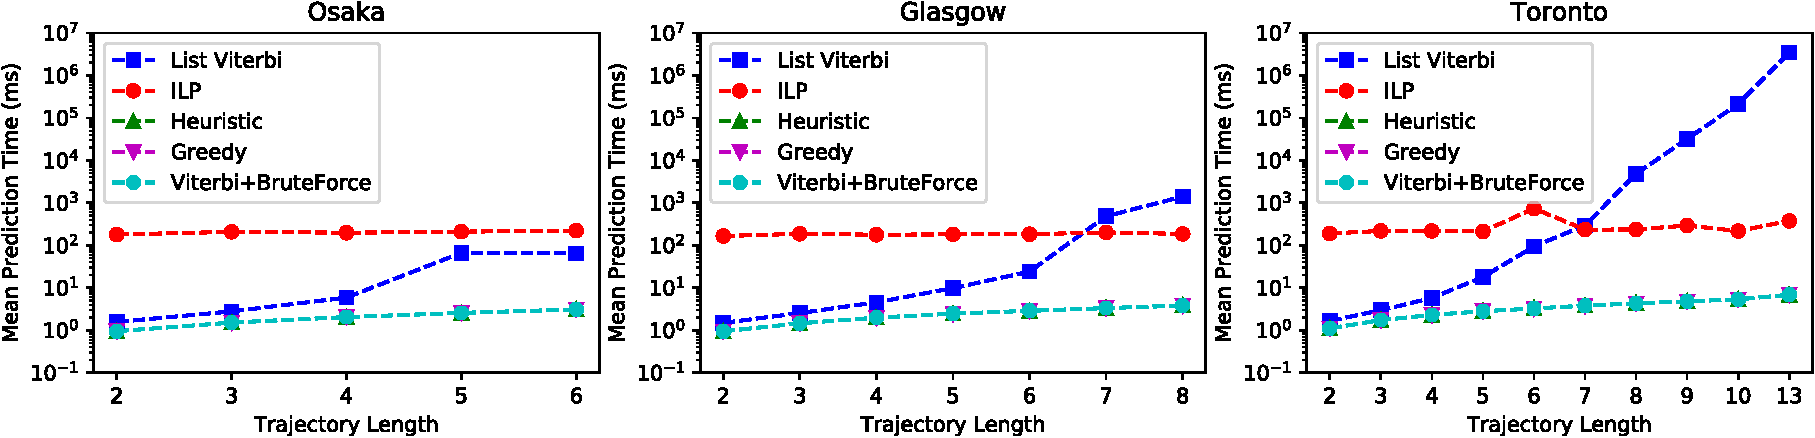
\includegraphics[width=\textwidth]{top1_inftime.pdf}
	    \captionof{figure}{Prediction time for three inference algorithms (in milliseconds)}
	    \label{fig:inftime}
	    %\captionmoveup\eqmoveup
%\end{figure*}%
%\begin{figure*}[!t]
		\quad
		\centering
		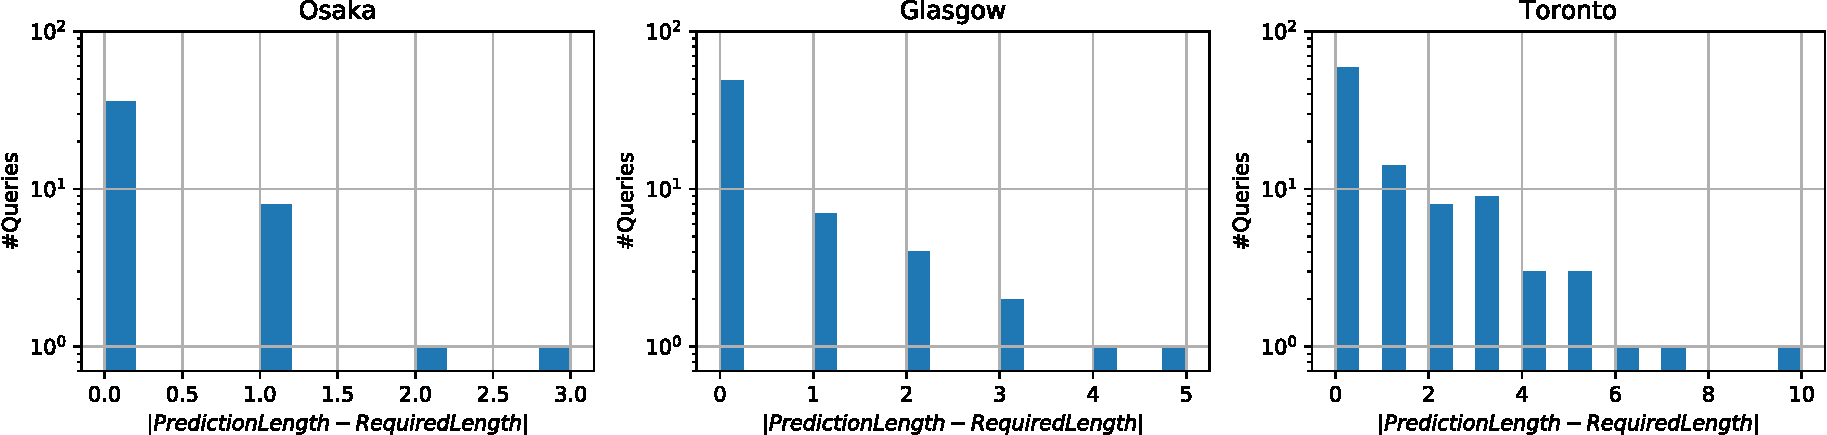
\includegraphics[width=\textwidth]{heu_lengthdiff.pdf}
	    \captionof{figure}{The difference between recommendation and required sequence length.}
	    \label{fig:length-christo}
	    %\captionmoveup\eqmoveup
%\end{figure*}%
%\begin{figure*}[!t]
		\quad
		\centering
		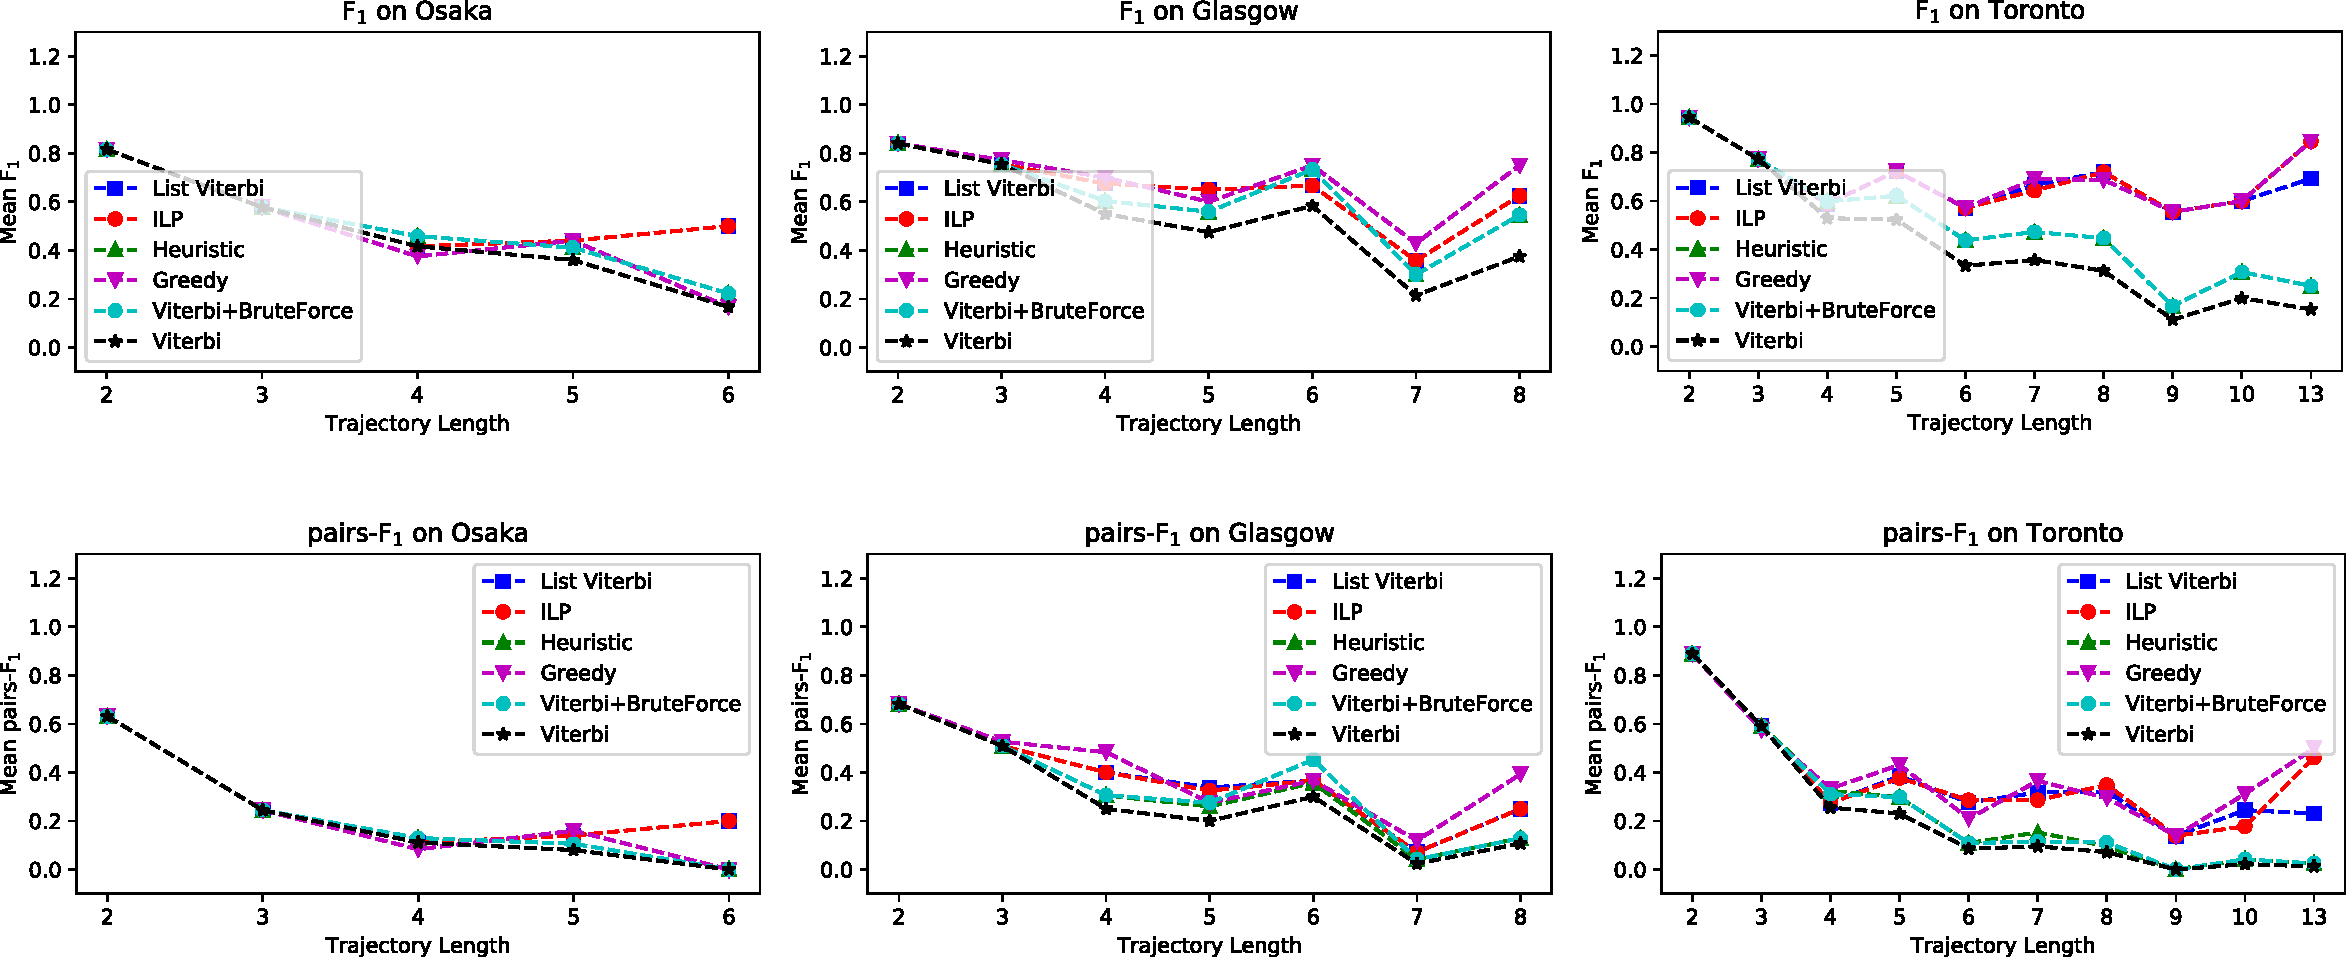
\includegraphics[width=\textwidth]{metrics.pdf}
		% 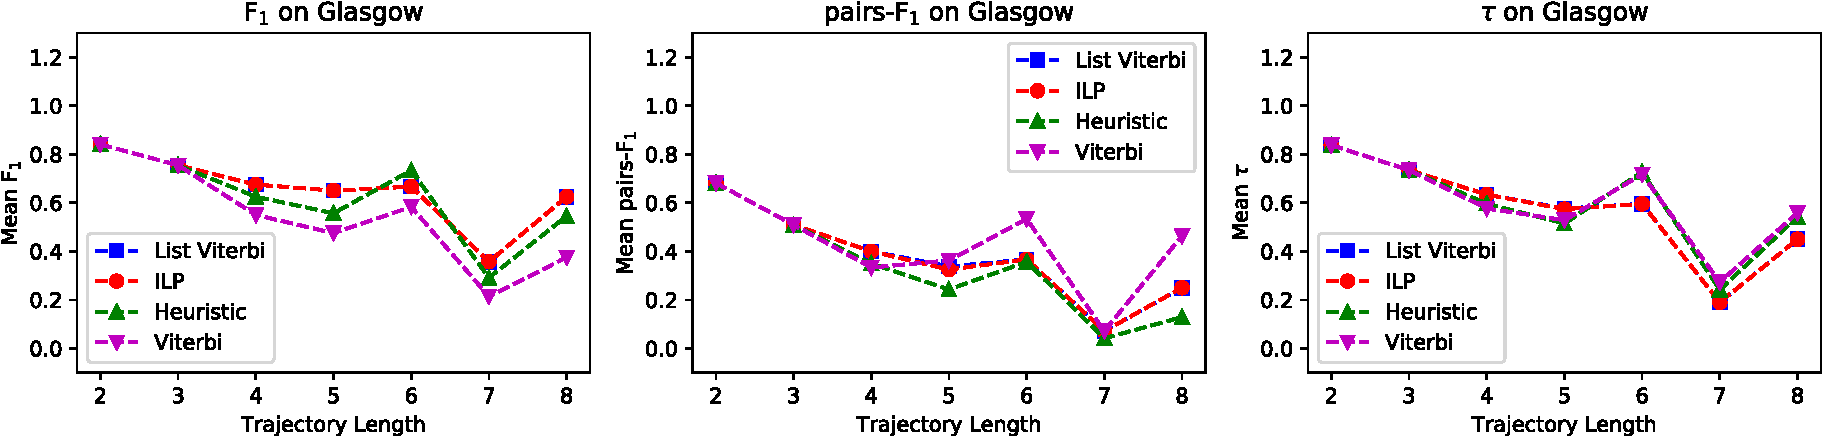
\includegraphics[width=\textwidth]{metric_d2.pdf}
		% 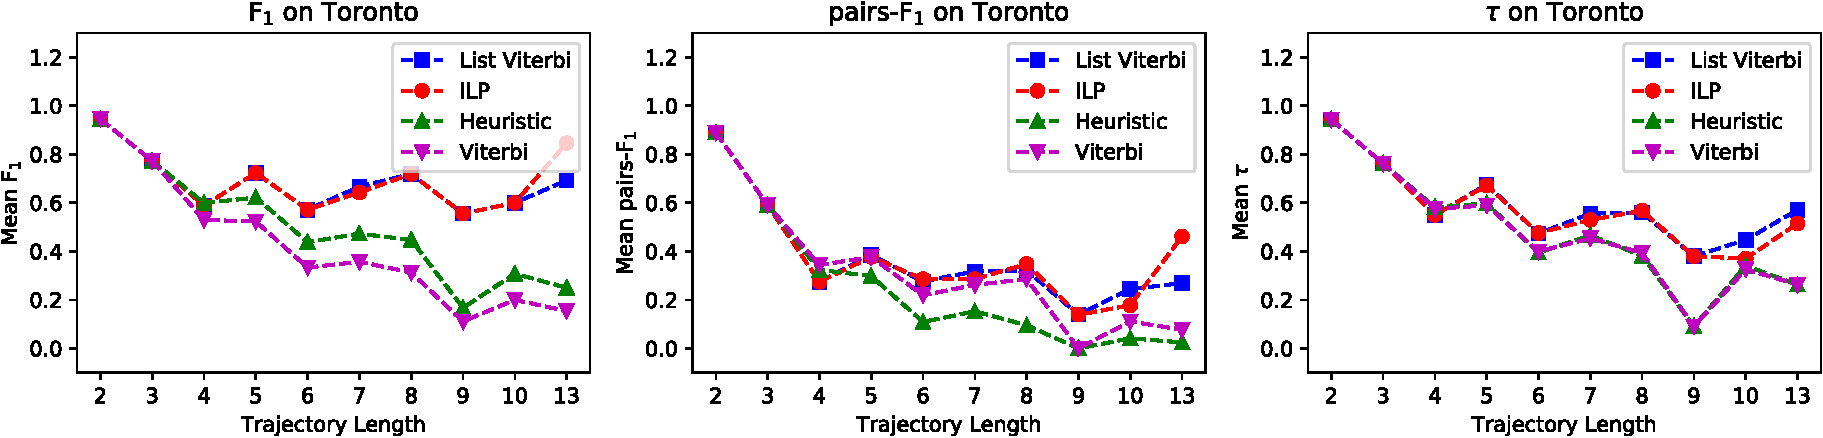
\includegraphics[width=\textwidth]{metric_d3.pdf}
	    \captionof{figure}{Accuracy versus trajectory length.}
	    \label{fig:acc-vs-length}
	    %\captionmoveup\eqmoveup
%\end{figure*}
\end{minipage}
\end{figure*}


%% 1. Recommend songs for playlists
% Problems description
% - playlist augmentation
% - new song recommendation
% - related work: the same, the different
%
% 2. Playlist augmentation and bipartite ranking
% Method:
% - augment one playlist can be achieved by bipartite ranking (assume order of tracks is irrelevant)
% - known: bipartite ranking == binary classification (under assumptions)
% - Theorem 1
% 
% 3. Playlist augmentation and multi-label classification
% Method:
% - augment multiple playlists -> multiple bipartite ranking -> multi-label classification
% - Theorem 2
% - one user has multiple playlists -> multi-task regularisation
%
% 4. New song recommendation: an extension of playlist augmentation
% Method:
% - the same as previous work (cold start)
% - the different (?)
%
% 5. Experiment
% - multi-label classification
% - playlist augmentation
% - new song recommendation
% 1. Recommend songs for playlists
% Problems description
% - playlist augmentation
% - new song recommendation
% - related work: the same, the different
%

\section{Problem}

% brief description of both recommendation tasks
We are motivated by the problem of automatically augmenting music playlist with a collection of songs $\SCal$,
in particular, given a partial playlist with the first $K$ songs\footnote{$K$ can be different for different partial playlists.},
we would like to recommend a subset of $\SCal$ by learning from user created playlist dataset.
This task is also known as Automatic Playlist Continuation~\cite{schedl2017,recsysch2018}.


\section{Related work}
% related work
% describe each task with related work: the same, the different
% describe that we don't use the order of songs, conflicting findings in literature
% mainly two pieces of work:
% - music recommendation
% - playlist generation
{\it Some related work.}

In this paper, we describe two variants of the playlist recommendation problem,
one is augmenting a playlist by recommending a subset of songs from a collection of music $\SCal$,
given the first $K$ seed songs, where $K$ can be any positive integer from 1 to the total number of songs in playlist minus 1.
% in contrast to settings where all songs except the last one are observed\cite{}, or giving a fixed number of seed songs\cite{}.
Another variant is restricting that all songs to recommend are not observed during learning,
\ie in the setting of recommending newly released songs to augment a given playlist, which is an instance of the cold-start problem.
We call the first variant \emph{playlist augmentation} and the second \emph{new song recommendation}.


\section{Machine learning tasks for playlist recommendation}

We formulate the task of \emph{playlist augmentation} as a multi-label classification problem,
that is, for each song that is not in the given playlist, 
we predict whether it will be added to the given playlist.
This formulation is illustrated in Figure~\ref{fig:pla},
where rows represent songs (no specific order) and columns represent playlists (no specific order).
Further, columns with white colour represent playlists in training set, 
and columns with grey colour represent playlists that should be augmented (\ie test set).
If entry $(i, j)$ is \texttt{1} (or \texttt{0}), 
it means the $i$-th song is (or not) found in the $j$-th playlist, 
and a question mark \texttt{?} means that we do not know whether the $i$-th song is found in the $j$-th playlist.
As a remark, columns represent playlists in test set contain only \texttt{1} and \texttt{?} entries.

\begin{figure}[!h]
\centering
\newcolumntype{a}{>{\columncolor[gray]{0.9}}c}  % define a new column type
\setlength{\tabcolsep}{1pt} % tweak the space between columns
%\begin{tabular}{|*{7}{c}|ccccc|} \hline
\begin{tabular}{|*{7}{c}|aaaaa|} \hline
%\rule{.3em}{0pt} 
\rule{0em}{10pt}
& \texttt{0} & \texttt{1} & \texttt{0} & $\cdots$ & \texttt{0} & & & \texttt{?} & $\cdots$ & \texttt{?} & \\
& \texttt{0} & \texttt{0} & \texttt{0} & $\cdots$ & \texttt{0} & & & \texttt{1} & $\cdots$ & \texttt{?} & \\
& \texttt{1} & \texttt{0} & \texttt{0} & $\cdots$ & \texttt{0} & & & \texttt{?} & $\cdots$ & \texttt{?} & \\
%\vspace{-5pt}
\vspace{-3pt}
& \texttt{0} & \texttt{0} & \texttt{0} & $\cdots$ & \texttt{1} & & & \texttt{?} & $\cdots$ & \texttt{1} & \\
& $\vdots$ & $\vdots$ & $\vdots$ & $\vdots$ & $\vdots$ & & & $\vdots$ & $\vdots$ & $\vdots$ & \\
& \texttt{0} & \texttt{0} & \texttt{1} & $\cdots$ & \texttt{0} & & & \texttt{?} & $\cdots$ & \texttt{?} & \\ \hline
\end{tabular}
\caption{Illustration of playlist augmentation as multi-label classification.}
\label{fig:pla}
\end{figure}



\paragraph{New song recommendation}
We formulate the task of \emph{new song recommendation} as a multi-label classification problem, 
where we predict, for each song in test set,
whether it will be included in a given playlist.
This formulation is illustrated in Figure~\ref{fig:mlr},
where rows represent songs (from top to bottom, sorted by the release date in ascending order)
and columns represent playlists (no specific order).
Further, rows with white colour represent songs in training set, and rows with grey colour represent songs in test set.
If entry $(i, j)$ is \texttt{1} (or \texttt{0}), it means the $i$-th song is (or not) found in the $j$-th playlist,
otherwise, we do not know whether the $i$-th song is found in the $j$-th playlist (\ie entry $(i, j)$ is a question mark \texttt{?}).
As a remark, we do not care about the order of songs in a playlist.

\begin{figure}[!h]
\centering
\setlength{\tabcolsep}{1pt} % tweak the space between columns
\begin{tabular}{|*{10}{c}|} \hline
%\rule{.3em}{0pt} 
\rule{0em}{10pt}
& \texttt{0} & \texttt{0} & \texttt{0} & \texttt{1} & \texttt{0} & $\cdots$ & $\cdots$ & \texttt{0} & \\
& \texttt{1} & \texttt{0} & \texttt{0} & \texttt{0} & \texttt{0} & $\cdots$ & $\cdots$ & \texttt{0} & \\
\vspace{-5pt}
& \texttt{0} & \texttt{0} & \texttt{0} & \texttt{0} & \texttt{0} & $\cdots$ & $\cdots$ & \texttt{1} & \\
& $\vdots$ & $\vdots$ & $\vdots$ & $\vdots$ & $\vdots$ & $\vdots$ & $\vdots$ & $\vdots$ & \\
& \texttt{0} & \texttt{0} & \texttt{0} & \texttt{0} & \texttt{1} & $\cdots$ & $\cdots$ & \texttt{0} & \\ \hline
%\rowcolor{gray!20}
\rowcolor[gray]{0.9}
%\vspace{-5pt}
\vspace{-3pt}
& \texttt{?} & \texttt{?} & \texttt{?} & \texttt{?} & \texttt{?} & $\cdots$ & $\cdots$ & \texttt{?} & \rule{0em}{10pt} \\
%\rowcolor{gray!20}
\rowcolor[gray]{0.9}
& $\vdots$ & $\vdots$ & $\vdots$ & $\vdots$ & $\vdots$ & $\vdots$ & $\vdots$ & $\vdots$ &  \\
%\rowcolor{gray!20}
\rowcolor[gray]{0.9}
& \texttt{?} & \texttt{?} & \texttt{?} & \texttt{?} & \texttt{?} & $\cdots$ & $\cdots$ & \texttt{?} & \\ \hline
\end{tabular}
\caption{Illustration of recommending new songs to augment playlists as multi-label classification.}
\label{fig:mlr}
\end{figure}




\section{Method I: Playlist augmentation as multi-label classification}
{\it Two methods are described here, but only one of them is necessary for this paper.}


% so we can just do multiple bipartite ranking for these two problems?
% we can actually do better than this, given \ref{ertekin2011equivalence} showed that P-Classification == P-Norm Push, 
% we have (equivalence in binary setting) and (extend the equivalence to multi-label setting)
% so 
% - an independent  bipartite ranking seems to be a better baseline?
% - bottom push on MLC dataset?
% - Theorem 1
\section{Classification vs. bipartite ranking}
\label{sec:binary}


\subsection{P-Classification loss vs. P-Norm Push loss}
\label{ssec:pc=pn}

Given a binary dataset $\DCal = \SCal_+ \cup \SCal_-$, where $\SCal_+$ is a set of positive examples, 
\ie $\SCal_+ = \{(x_+, +1)\}$, and $\SCal_-$ is a set of negative examples, \ie $\SCal_- = \{(x_-, -1)\}$.

The empirical risk of the P-Classification loss is defined as~\cite{ertekin2011equivalence}
\begin{equation*}
\RCal_\textsc{pc}(\w, b) 
= \sum_{x_+ \in \SCal_+} e^{- (\w^\top x_+ + b)} +
  \frac{1}{p} \sum_{x_- \in \SCal_-} e^{p (\w^\top x_- + b)},
\end{equation*}
where $p > 0$ is a parameter.

The empirical risk of the P-Norm Push loss is defined as~\cite{rudin2009p}
\begin{equation*}
\begin{aligned}
\RCal_\textsc{pn}(\w)
&= \sum_{x_+ \in \SCal_+} \sum_{x_- \in \SCal_-} e^{-(\w^\top x_+ - \w^\top x_-)} \\
&= \sum_{x_+ \in \SCal_+} e^{-\w^\top x_+} \sum_{x_- \in \SCal_-} e^{\w^\top x_-}.
\end{aligned}
\end{equation*}

\citep{ertekin2011equivalence} showed the following equivalence relationship between P-Classification loss and P-Norm Push loss:
\begin{theorem}
\label{th:pc=pn}
If $(\w_\textsc{pc}, b_\textsc{pc}) \in \argmin_{\w,b} \RCal_\textsc{pc}(\w, b)$, 
then $\w_\textsc{pc} \in \argmin_\w \RCal_\textsc{pn}(\w)$.
Further, If $\w_\textsc{pn} \in \argmin_\w \RCal_\textsc{pn}(\w)$, 
then $(\w_\textsc{pn}, b_\textsc{pn}) \in \argmin_{\w,b} \RCal_\textsc{pn}(\w, b)$ where
$$
b_\textsc{pn} 
= \frac{1}{p + 1} \left( 
  \ln \sum_{x_+ \in \SCal_+} e^{-\w_\textsc{pn}^\top x_+} - 
  \ln \sum_{x_- \in \SCal_-} e^{p\w_\textsc{pn}^\top x_-} \right).
$$
\end{theorem}

It turns out Theorem~\ref{th:pc=pn} is due to a general equivalence relationship 
between binary classification and bipartite ranking, which we detail in the next section.



\subsection{Binary classification loss vs. bipartite ranking loss}

Let function $f(\cdot, \cdot)$ be
$$
f(x; \w) := g(x; \w) + b,
$$
where $\x$ is an input, $\w$ is a weight vector, $b$ is a bias parameter, 
and function $g(x; \w)$ is differentiable (w.r.t. $\w$) and bounded.

Suppose $\alpha, \beta, c, P, Q \in \R_+$ are \emph{finite} positive numbers, we define 
$\RCal_\textsc{bc}$ be the following classification risk\footnote{
We note that there is a equivalent definition:
$\RCal_\textsc{bc}(\w) = \frac{1}{\alpha} \sum_{x_+ \in \SCal_+} \exp(-\alpha f(x_+; \w)) + 
\frac{C}{\beta} \sum_{x_- \in \SCal_-} \exp( \beta f(x_-; \w))$
where $C = Q/P$, since multiplying a positive constant to a loss function will not change its minimiser.}
:
\begin{equation*}
%\label{eq:bc}
\resizebox{\linewidth}{!}{$
%\begin{aligned}
\RCal_\textsc{bc}(\w, b)
= \displaystyle 
  \frac{P}{\alpha} \sum_{x_+ \in \SCal_+} e^{-\alpha f(x_+; \w)} +
  \frac{Q}{\beta}  \sum_{x_- \in \SCal_-} e^{ \beta  f(x_-; \w)},
%\end{aligned}
$}
\end{equation*}
and let
$\RCal_\textsc{br}$ be a bipartite ranking risk defined as:
\begin{equation*}
%\label{eq:br}
\resizebox{\linewidth}{!}{$
\begin{aligned}
\RCal_\textsc{br}(\w)
&= \left[ \displaystyle 
   \sum_{x_+ \in \SCal_+} \left( \sum_{x_- \in \SCal_-} e^{-\beta (f(x_+; \w) - f(x_-; \w))} \right)^\frac{\alpha}{\beta} 
   \right]^c \\
&= \left[ \sum_{x_+ \in \SCal_+} e^{-\alpha f(x_+; \w)} \right]^\frac{c}{\alpha}
   \left[ \sum_{x_- \in \SCal_-} e^{ \beta  f(x_-; \w)} \right]^\frac{c}{\beta}.
\end{aligned}
$}
\end{equation*}
Note that $\RCal_\textsc{br}$ is independent of $b$.


\begin{theorem}
\label{th:bc=br}
If $(\w_\textsc{bc}, b_\textsc{bc}) \in \argmin_{\w,b} \RCal_\textsc{bc}(\w, b)$,
then $\w_\textsc{bc} \in \argmin_\w \RCal_\textsc{br}(\w)$, and
$$
\resizebox{\linewidth}{!}{$
\displaystyle
b_\textsc{bc} 
= \frac{1}{\alpha + \beta} \left( 
  P \ln \sum_{x_+ \in \SCal_+} e^{-\alpha g(x_+; \w_\textsc{bc})} -
  Q \ln \sum_{x_- \in \SCal_-} e^{  \beta g(x_-; \w_\textsc{bc})} \right).
$}
$$
Further, if $\w_\textsc{br} \in \argmin_\w \RCal_\textsc{br}(\w)$ (assuming minimisers exist),
then $(\w_\textsc{br}, b_\textsc{br}) \in \argmin_{\w,b} \, \RCal_\textsc{bc}(\w, b)$, where
$$
\resizebox{\linewidth}{!}{$
\displaystyle
b_\textsc{br} 
= \frac{1}{\alpha + \beta} \left( 
  P \ln \sum_{x_+ \in \SCal_+} e^{-\alpha g(x_+; \w_\textsc{br})} -
  Q \ln \sum_{x_- \in \SCal_-} e^{  \beta g(x_-; \w_\textsc{br})} \right).
$}
$$
\end{theorem}

We can get Theorem~\ref{th:pc=pn} from Theorem~\ref{th:bc=br} by letting $\alpha=c=P=Q=1$ and $\beta=p$.
Moreover, Theorem~\ref{th:bc=br} summaries a few more well-known special cases.

\TODO

{\it Cost-sensitive AdaBoost == RankBoost, Theorem 3 of~\cite{ertekin2011equivalence}.
IR Push == P-Classification,
IR Push = Top Push + exponential surrogate + log-sum-exp, P-Norm Push vs. Top Push vs. IR Push (approximation inside/outside)
Bottom Push + exponential surrogate + log-sum-exp == a classification loss similar to P-Classification.
}

\begin{table}[!h]
\centering
\caption{Summary of parameters for the equivalence of (risk of rank loss, risk of classification loss) pairs}
\label{tab:config}
\begin{tabular}{r*{6}{c}}
\toprule
{\bf Loss pairs}                                         & $\alpha$ & $\beta$ & $\gamma$ & $\delta$ & $P$ & $Q$ \\ \hline
$\RCal_\textsc{pn} \equiva \RCal_\textsc{pc}$            & $1$      & $p$     & $p$      & $1$      & $\frac{1}{p}$ & $\frac{1}{p}$ \\
$\widetilde\RCal_\textsc{tp} \equiva \RCal_\textsc{pc}$  & $1$      & $r=p$   & $1$      & $\frac{1}{r}=\frac{1}{p}$ & $1$ & $1$ \\
$\widetilde\RCal_\textsc{bp} \equiva \RCal_\textsc{rc}$  & $r=q$    & $1$     & $\frac{1}{r}=\frac{1}{q}$ & $1$ & $1$ & $1$ \\
$\widetilde\RCal_\textsc{csa} \equiva \RCal_\textsc{rb}$ & $1$      & $1$     & $1$      & $1$      & $1$ & $C$ \\
\bottomrule
\end{tabular}
\end{table}




% 3. Playlist augmentation and multi-label classification
% Method:
% - augment multiple playlists -> multiple bipartite ranking -> multi-label classification
% - Theorem 2
% - one user has multiple playlists -> multi-task regularisation
%
\documentclass[9pt]{extarticle}
\usepackage[a4paper,top=0.79in,left=0.79in,bottom=0.79in,right=0.79in]{geometry} % A4 paper margins in LibreOffice
\usepackage[numbers,compress]{natbib}
\usepackage{hyperref}
\usepackage{mathtools}
\usepackage{amsthm}
\usepackage{amsfonts}
\usepackage{mathrsfs}
\usepackage{bm}
\usepackage{bbm}
%\usepackage{ulem}
\usepackage{stmaryrd}
\usepackage{algorithm}
\usepackage{algorithmic}
\usepackage[sc]{mathpazo}
\linespread{1.05}       % Palladio needs more leading (space between lines)
\usepackage[T1]{fontenc}
\usepackage{footmisc}   % \footref, refer the same footnote at different places
\usepackage{subcaption} % sub-figures
\usepackage{setspace}   % set space between lines
\usepackage[utf8]{inputenc}
\usepackage[english]{babel}
\usepackage{xcolor}
\usepackage{graphicx}
\graphicspath{{fig/}}   % Location of the graphics files

\newtheorem{theorem}{Theorem}
\newtheorem{corollary}{Corollary}
\newtheorem{lemma}{Lemma}

\DeclareMathOperator*{\argmin}{argmin}
\DeclareMathOperator*{\argmax}{argmax}
\newcommand{\eat}[1]{}
\newcommand{\given}{\mid}
\newcommand{\llb}{\llbracket}
\newcommand{\rrb}{\rrbracket}
\newcommand{\bu}{\mathbf{u}}
\newcommand{\bv}{\mathbf{v}}
\newcommand{\f}{\mathbf{f}}
\newcommand{\h}{\mathbf{h}}
\newcommand{\x}{\mathbf{x}}
\newcommand{\y}{\mathbf{y}}
\newcommand{\z}{\mathbf{z}}
\newcommand{\1}{\mathbf{1}}
\newcommand{\w}{\mathbf{w}}
\newcommand{\A}{\mathbf{A}}
\newcommand{\B}{\mathbf{B}}
\newcommand{\W}{\mathbf{W}}
\newcommand{\X}{\mathbf{X}}
\newcommand{\Y}{\mathbf{Y}}
\newcommand{\p}{\mathbb{P}}
\newcommand{\E}{\mathbb{E}}
\newcommand{\R}{\mathbb{R}}
\newcommand{\Z}{\mathbb{Z}}
\newcommand{\q}{\mathbf{q}}
\newcommand{\LCal}{\mathcal{L}}
\newcommand{\SCal}{\mathcal{S}}
\newcommand{\XCal}{\mathcal{X}}
\newcommand{\YCal}{\mathcal{Y}}
\newcommand{\alphat}{\widetilde{\alpha}}
\newcommand{\betat}{\widetilde{\beta}}
\newcommand{\gammat}{\widetilde{\gamma}}
\newcommand{\phit}{\widetilde{\phi}}
\newcommand{\alphabm}{\bm{\alpha}}
\newcommand{\betabm}{\bm{\beta}}
\newcommand{\nubm}{\bm{\nu}}
\newcommand{\xibm}{\bm{\xi}}
\newcommand{\thetabm}{\bm{\theta}}
\newcommand{\one}{\mathbf{1}}
% madeness: suPer-script in Brackets
\newcommand{\pb}[1]{^{({#1})}}

\newcommand{\eg}{e.g.\ }
\newcommand{\ie}{i.e.\ }
\newcommand{\downto}{\,\textbf{downto}\,}
\newcommand{\blue}[1]{{\color{blue}{#1}}}

\setlength{\columnsep}{1.5em} % spacing between columns

\title{Multi-label Classification, Bipartite Ranking and Playlist Generation}

\author{Dawei Chen}

\date{\today}

\begin{document}

\maketitle

\section{Multi-label classification}
\label{sec:mlc}

%1. Brief summary of reference
\paragraph{Summary}
\citet{dembczynski:2010} formalised the multi-label classification problem, 
and claimed that if Hamming loss or rank loss is used,
multi-label classification methods, in theory, could not benefit from modelling label dependence.
On the other hand, modelling correlation between labels was necessary if one chose to use the subset 0/1 loss.
Further, a probabilistic classifier chains (PCC), which generalised the classifier chains (CC) from a probabilistic perspective,
was proposed to modelling label correlation. 

Theoretically, the order of labels does not affect the model, 
in practice, however, using different order of labels will result in different model parameters (we do not have infinity data).
To alleviate this issue, an ensemble of PCC (EPCC) was proposed, which made a prediction by averaging over predictions by a number of PCCs, 
each model was trained using a randomly chosen permutation of the labels.
PCC (and EPCC) was empirically shown to outperform a number of baselines that did not model label correlations when label dependence existed in data.


\noindent
\paragraph{Definition}
Let $\LCal = \{\lambda_1,\dots,\lambda_l\}$ be a finite set of class labels,
and example $(\x,\y) \in \XCal \times \YCal$, 
where $\YCal \in \{0,1\}^m$ is the set of all possible labels,
and $\y=y_{1:m}$ is a binary vector where $y_i = 1$ \emph{iff} $\lambda_i$ is a label of $\x$.
A multi-label classifier is a mapping $\h: \XCal \to \YCal$.

\noindent
\paragraph{Label dependence}
Suppose examples are independent and identically distributed (iid) according to a joint probability distribution $\p(\X,\Y)$ on $\XCal \times \YCal$,
where $\X$ is a random variable and $\Y=Y_{1:l}$ is a random vector,
Let $\p\pb{i}(Y_i |\x)$ be the marginal distribution of $Y_i$, then
\begin{equation*}
\p\pb{i}(Y_i=b |\x) = \sum_{\y \in \YCal:y_i = b} \p(\Y = \y |\x),
\end{equation*}
where $\p(\Y = \y |\x)$ is the posterior distribution given observation $\x$.
We note that the labels are not independent if 
\begin{equation*}
\p(\Y |\x) \ne \prod_{i=1}^l \p\pb{i}(Y_i |\x),
\end{equation*}
and the degree of dependence could be quantified in terms of measures such as cross entropy and KL divergence.

\noindent
\paragraph{Learning}
Given a loss function $\ell(\cdot)$, 
we can learn a multi-label classifier by find a model $\h^*$ that minimise the expected loss over the joint distribution $\p(\X,\Y)$:
\begin{equation*}
\h^* 
= \argmin_{\h} \, \E_{\X\Y} \, \ell(\Y,\h(\X))
= \argmin_{\h} \, \E_{\X} \, \E_{\Y|\X} \, \ell(\Y,\h(X))
= \argmin_{\h} \, \sum_{\x} \x \p(\x) \, \E_{\Y|\X} \, \ell(\Y,\h(\x)),
\end{equation*}
thanks to the summation, fix $\x$, we have
\begin{equation*}
\h^*(\x) = \argmin_{\y} \, \E_{\Y|\X} \, \ell(\Y,\y).
\end{equation*}
Frequently used loss functions in the context of multi-label classification including Hamming loss, rank loss and subset 0/1 loss~\cite{dembczynski:2010},
here we focus on a rank loss (taking care of ties):
\begin{equation}
\label{eq:loss_rank}
\ell(\y, \h(\x)) = \sum_{(i,j): y_i > y_j} \left( \llb h_i < h_j \rrb + \frac{1}{2} \llb h_i = h_j \rrb \right).
\end{equation}
\emph{Theorem 3.1 in~\cite{dembczynski:2010} here.}

\noindent
\paragraph{Probabilistic classifier chains}
Given a query $\x$, the posterior probability of a label $\y$ can be computed using the product rule of probability:
\begin{equation*}
\p(\y |\x) = \p(y_1) \cdot \prod_{i=2}^l \p(y_i |\x, y_{1:i-1}),
\end{equation*}
and we further define a function:
\begin{equation*}
f_i = 
\begin{cases}
\p(y_i = 1 |\x), & i = 1 \\
\p(y_i = 1 |\x, y_{1:i-1}), & 1 < i \le l
\end{cases}
\end{equation*}
then we have
\begin{equation*}
\p(\y |\x) = f_1 \cdot \prod_{i=2}^l f_i,
\end{equation*}
where $f_i$ uses $\x$ and $y_{1:i-1}$ as the input features. 
Theoretically, the results of the product rule does not depend on the order of variables, 
however, in practice, different order of variables will result in different model parameters (\ie the order of features depend on the order of variables). \\
\emph{Greedy approach -- classifier chain; assuming Markov property, we can use the Viterbi algorithm; with Neural net, we can build an order agnostic model.}


\section{Bipartite ranking}
\label{sec:birank}

%1. Brief summary of reference
\paragraph{Summary}
\citet{li:2014} proposed a new algorithm (\ie \emph{TopPush}) for bipartite ranking to optimise the ranking accuracy at the top.
This algorithm has a linear time complexity at each iteration of the optimisation process.

The key observation was that the loss used in~\cite{agarwal:2011} (when indicator function is replaced with a convex surrogate)
can be equivalently transformed to a new form 
which can be optimised in linear time (w.r.t the size of training set).


\paragraph{Definition} 
Bipartite ranking is to learn a real-valued ranking function that places positive examples above negative examples~\cite{li:2014}.
Formally, given training examples $S = S_+ \cup S_-$ with $m$ positive examples $S_+ = \{\x_i^+\}_{i=1}^m$ and $n$ negative examples $S_- = \{\x_i^-\}_{i=1}^n$, 
bipartite ranking aims to learn a ranking function $f: \XCal \to \R$ that is likely ranks positive examples higher than negative examples.

\paragraph{Loss function}
AUC is a widely used as an evaluate metric for bipartite ranking, and it turns out that AUC can be optimised by minimising a loss defined as~\cite{cortes:2004}
\begin{equation}
\label{eq:loss_auc}
\ell_\text{rank}(f; S) = \frac{1}{mn} \sum_{i=1}^m \sum_{j=1}^n \llb f(\x_i^+) \le f(\x_j^-) \rrb,
\end{equation}
and this loss can be easily optimised (\eg by gradient descent) if we replace the indicator function with a convex surrogate such as the truncated quadratic loss 
$\ell(z) = (1+z)_+^2$, the exponential loss $\ell(z) = e^z$ and logistic loss $\ell(z) = \log(1+e^z)$.
One drawback of this loss function is enumerating all the positive-negative pairs, which is computationally expensive for large dataset. \\
\emph{Theorem 3.1 in~\cite{dembczynski:2010} for this loss function here.}

Alternatively, one may interested in optimising the ranking accuracy only at the top, 
or equivalently, we would like to minimize the number of positive examples that ranked below the highest-ranking negative instance~\cite{agarwal:2011,li:2014}:
\begin{equation}
\label{eq:loss_inf}
\begin{aligned}
\ell_{\infty}(f; S) 
&= \max_{1 \le j \le n} \frac{1}{m} \sum_{i=1}^m \, \llb f(\x_i^+) < f(\x_j^-) \rrb \\
&= \frac{1}{m} \sum_{i=1}^m \max_{1 \le j \le n} \llb f(\x_i^+) < f(\x_j^-) \rrb,
\end{aligned}
\end{equation}
by replace the indicator function in (\ref{eq:loss_inf}) with a convex surrogate $\ell(\cdot)$, we have
\begin{equation}
\label{eq:loss_inf1} 
\begin{aligned}
\tilde{\ell}_{\infty}(f; S) 
&= \frac{1}{m} \sum_{i=1}^m \max_{1 \le j \le n} \ell\left( f(\x_j^-) - f(\x_i^+) \right) \\
&= \frac{1}{m} \sum_{i=1}^m \ell\left( \max_{1 \le j \le n} f(\x_j^-) - f(\x_i^+) \right),
\end{aligned}
\end{equation}
which can be optimised more efficiently than (\ref{eq:loss_auc})~\cite{li:2014}.

\paragraph{Dual formulation}
Consider a linear ranking function $f(\x) = \w^\top \x$ and loss function~\ref{eq:loss_inf1}.
Table~\ref{tab:symbol} summarises some notation we will use.
\begin{table}[!h]
\caption{Glossary of commonly used symbols}
\label{tab:symbol}
\renewcommand{\arraystretch}{1.5} % tweak the space between rows
\setlength{\tabcolsep}{1pt} % tweak the space between columns
\centering
\begin{tabular}{llll}
\hline \hline
\multicolumn{3}{l}{\textbf{Symbol}} & \textbf{Quantity} \\ \hline 
$d$              &  $\in$  &  $\Z^+$  & The number of features for each example \\
$\w$             &  $\in$  &  $\R^d$  & The vector of model parameters \\
$\mathbf{1}_m$   &  $\in$  &  $\R^m$  & The $m$ dimensional vector of $1$'s \\
$\X^+$           &  $\in$  &  $\R^{m \times d}\quad$  & Matrix of features of positive examples \\
$\X^-$           &  $\in$  &  $\R^{n \times d}$       & Matrix of features of negative examples \\
$\alphabm$       &  $\in$  &  $\R^m$  &  Dual variables for positive examples \\
$\betabm, \nubm$ &  $\in$  &  $\R^n$  &  Dual variables for negative examples \\ \hline
\end{tabular}
\end{table}

We can learn the model parameters $\w$ by risk minimisation with L2 regularisation:
\begin{equation}
\label{eq:minrisk}
\min_{\w} \, \frac{\lambda}{2} \w^\top \w + \frac{1}{m} \sum_{i=1}^m \ell\left( \max_{1 \le j \le n} \w^\top \x_j^- - \w^\top \x_i^+ \right),
\end{equation}
where $\lambda > 0$ is a regularisation constant.
Problem (\ref{eq:minrisk}) is hard to optimise in general due to the maximum term in loss function, one widely used trick is to form its dual problem.
Let 
\begin{equation*}
\begin{aligned}
f_0 (\w, \xi) &= \frac{\lambda}{2} \w^\top \w + \frac{1}{m} \sum_{i=1}^m \ell\left( \xi - \w^\top \x_i^+ \right), \\
f_j (\w, \xi) &= \w^\top \x_j^- - \xi, \ j \in \{1,\dots,n\}.
\end{aligned}
\end{equation*}
Then problem (\ref{eq:minrisk}) is equivalent to
\begin{equation}
\label{eq:minrisk_lg}
\begin{aligned}
\min_{\w, \xi} \quad & f_0 (\w, \xi) \\
s.t. \quad & f_j (\w, \xi) \le 0, \ j \in \{1,\dots,n\}.
\end{aligned}
\end{equation}
For $\nu_j \ge 0, \, j \in \{1,\dots,n\}$, the \emph{Lagrangian} of (\ref{eq:minrisk_lg}) is
\begin{equation}
\label{eq:minrisk_lg1}
\begin{aligned}
L(\w, \xi, \nubm) 
&= f_0 (\w, \xi) + \sum_{j=1}^n \nu_j \cdot f_j(\w, \xi) \\
&= \frac{\lambda}{2} \w^\top \w + \frac{1}{m} \sum_{i=1}^m \ell\left( \xi - \w^\top \x_i^+ \right) + \sum_{j=1}^n \nu_j \cdot \left( \w^\top \x_j^- - \xi \right)
\end{aligned}
\end{equation}
Note that the conjugate of the conjugate of a convex function is itself, \ie $f(\z) = f^{**}(\z) = \sup_{\y} \left( \z^\top \y - f^*(\y) \right)$, we have
\begin{equation}
\label{eq:lg_part1}
\begin{aligned}
\frac{1}{m} \sum_{i=1}^m \ell\left( \xi - \w^\top \x_i^+ \right)
&= \frac{1}{m} \sum_{i=1}^m \sup_{\alpha_i} \left( (\xi - \w^\top \x_i^+) \cdot \alpha_i - \ell^*(\alpha_i) \right) \\
&= \sup_{\alphabm} \left[ \frac{1}{m} \sum_{i=1}^m (\xi - \w^\top \x_i^+) \cdot \alpha_i - \frac{1}{m} \sum_{i=1}^m \ell^*(\alpha_i) \right] \\
&= \sup_{\alphabm} \left[ \frac{\xi}{m} \1_m^\top \alphabm - \frac{1}{m} \alphabm^\top \X^+ \w - \frac{1}{m} \sum_{i=1}^m \ell^*(\alpha_i) \right] \\
\end{aligned}
\end{equation}
where $\ell^*(\cdot)$ is the conjugate of $\ell(\cdot)$.
Further, 
\begin{equation}
\label{eq:lg_part2}
\sum_{j=1}^n \nu_j \cdot \left( \w^\top \x_j^- - \xi \right) = \nubm^\top \X^- \w - \xi \1_n^\top \nubm
\end{equation}
Then by (\ref{eq:minrisk_lg1}), (\ref{eq:lg_part1}) and (\ref{eq:lg_part2}), we have
\begin{align*}
L(\w, \xi, \alphabm, \nubm) 
&= \frac{\lambda}{2} \w^\top \w + 
   \sup_{\alphabm} \left[ \frac{\xi}{m} \1_m^\top \alphabm - \frac{1}{m} \alphabm^\top \X^+ \w - \frac{1}{m} \sum_{i=1}^m \ell^*(\alpha_i) \right] +
   \nubm^\top \X^- \w - \xi \1_n^\top \nubm \\
&= \sup_{\alphabm} \left[ 
   \frac{\lambda}{2} \w^\top \w + 
   \frac{\xi}{m} \1_m^\top \alphabm - \frac{1}{m} \alphabm^\top \X^+ \w - \frac{1}{m} \sum_{i=1}^m \ell^*(\alpha_i) +
   \nubm^\top \X^- \w - \xi \1_n^\top \nubm \right] \\
&= \sup_{\alphabm} \left[ g(\w, \xi) - \frac{1}{m} \sum_{i=1}^m \ell^*(\alpha_i) \right]
\end{align*}
where
$$g(\w, \xi) = \frac{\lambda}{2} \w^\top \w + \frac{\xi}{m} \1_m^\top \alphabm - \frac{1}{m} \alphabm^\top \X^+ \w + \nubm^\top \X^- \w - \xi \1_n^\top \nubm$$
The \emph{Lagrangian dual function} of (\ref{eq:minrisk_lg}) is
\begin{equation}
\label{eq:lg_dual_func}
\begin{aligned}
\inf_{\w, \xi} \, L(\w, \xi, \alphabm, \nubm) 
&= \inf_{\w, \xi}  \, \sup_{\alphabm} \left[ g(\w, \xi) - \frac{1}{m} \sum_{i=1}^m \ell^*(\alpha_i) \right] \\
&= \sup_{\alphabm} \, \inf_{\w, \xi} \left[ g(\w, \xi) - \frac{1}{m} \sum_{i=1}^m \ell^*(\alpha_i) \right] ~~ \text{(assuming strong duality)} \\
&= \max_{\alphabm} \, \min_{\w, \xi} \left[ g(\w, \xi) - \frac{1}{m} \sum_{i=1}^m \ell^*(\alpha_i) \right] ~~ \text{(Equation (\ref{eq:minrisk}) is L2 regularised~\cite{shalev:2007})} \\
&= \max_{\alphabm} \left[ \min_{\w, \xi} g(\w, \xi) - \frac{1}{m} \sum_{i=1}^m \ell^*(\alpha_i) \right]
\end{aligned}
\end{equation}
To solve the (unconstrained) inner minimisation, let
\begin{align*}
\frac{\partial g}{\partial \w}  &= \lambda \w - \frac{1}{m} \left( \alphabm^\top \X^+ \right)^\top + \left( \nubm^\top \X^- \right)^\top = 0 \\
\frac{\partial g}{\partial \xi} &= \frac{1}{m} \1_m^\top \alphabm - \1_n^\top \nubm = 0
\end{align*}
Then we have
\begin{equation}
\label{eq:sol1}
\widetilde\w 
= \frac{1}{\lambda m} \left( \alphabm^\top \X^+ - m \nubm^\top \X^- \right)^\top 
= \frac{1}{\lambda m} \left( \alphabm^\top \X^+ - \betabm^\top \X^- \right)^\top  
\end{equation}
and
\begin{equation}
\label{eq:sol2}
\1_m^\top \alphabm = m \1_n^\top \nubm = \1_n^\top \betabm
\end{equation}
where $\betabm = m \nubm \succeq 0$, and by (\ref{eq:sol1}) and (\ref{eq:sol2}), we have
\begin{equation}
\label{eq:min_func}
\begin{aligned}
\min_{\w, \xi} g(\w, \xi) 
&= \frac{\lambda}{2} \widetilde\w^\top \widetilde\w + \frac{\xi}{m} \1_m^\top \alphabm -
   \frac{1}{m} \alphabm^\top \X^+ \widetilde\w + \nubm^\top \X^- \widetilde\w - \xi \1_n^\top \nubm \\
&= \frac{\lambda}{2} \widetilde\w^\top \widetilde\w + 
   \frac{\xi}{m} \left( \1_m^\top \alphabm - m \1_n^\top \nubm \right) - 
   \frac{1}{m} \left( \alphabm^\top \X^+ - m \nubm^\top \X^- \right) \widetilde\w \\
&= \frac{\lambda}{2} \widetilde\w^\top \widetilde\w + 0 - \lambda \widetilde\w^\top \widetilde\w \\
&= -\frac{\lambda}{2} \widetilde\w^\top \widetilde\w \\
&= -\frac{1}{2 \lambda m^2} \left\| \alphabm^\top \X^+ - \betabm^\top \X^- \right\|^2
\end{aligned}
\end{equation}
Lastly, by (\ref{eq:lg_dual_func}) and (\ref{eq:min_func}), the \emph{Lagrangian dual problem} of (\ref{eq:minrisk_lg}) is
\begin{align*}
\max_{\nubm} \, \inf_{\w, \xi} \, L(\w, \xi, \alphabm, \nubm) 
= \max_{\alphabm, \nubm} \, \left[ \min_{\w, \xi} g(\w, \xi) - \frac{1}{m} \sum_{i=1}^m \ell^*(\alpha_i) \right]
= \max_{\alphabm, \betabm} \, \left[ -\frac{1}{2 \lambda m^2} \left\| \alphabm^\top \X^+ - \betabm^\top \X^- \right\|^2 - 
  \frac{1}{m} \sum_{i=1}^m \ell^*(\alpha_i) \right]
\end{align*}
subject to $\1_m^\top \alphabm = m \1_n^\top \nubm$ and $\nubm \succeq 0$,
or equivalently 
\begin{equation}
\label{eq:minrisk_dual}
\begin{aligned}
\min_{\alphabm, \betabm} \quad & \frac{1}{2 \lambda m} \left\| \alphabm^\top \X^+ - \betabm^\top \X^- \right\|^2 + \sum_{i=1}^m \ell^*(\alpha_i) \\
s.t. \quad & \1_m^\top \alphabm = \1_n^\top \betabm \\
& \betabm \succeq 0.
\end{aligned}
\end{equation}


\section{Playlist generation as multi-label classification}
\label{sec:playlist}

%2. Formal problem statement (e.g. input, output)
%\subsection{Problem formulation}

Given $N$ playlists where songs in each playlist are from a music library with $K$ songs $\{s_i\}_{i=1}^K$,
we derive a training set $\SCal = \left\{ \left( \x\pb{n}, \y\pb{n} \right) \right\}_{n=1}^N$ where $\x\pb{n} \in \R^D$ is a feature vector of the query 
induced by the $n$-th playlist (\eg the feature vector of the first song in the $n$-th playlist),
$\y\pb{n} \in \{0,1\}^K$ is a binary indicator such that 
$$
y_i\pb{n} = 
\begin{cases}
1, & \text{song $s_i$ is in the $n$-the playlist} \\
0, & \text{otherwise}
\end{cases}
$$

The empirical risk of a predictor $\f$ (with parameters $\w$) on training set $\SCal$ is
\begin{equation}
\label{eq:risk_pl}
R_{\LCal}(\f; \SCal) = \frac{1}{N} \sum_{n=1}^N \LCal\left(\f(\x\pb{n}), \y\pb{n}\right),
\end{equation}
where $\LCal(\cdot)$ is a loss function for multi-label learning such as Hamming loss, rank loss, subset 0/1 loss etc.

For training example $(\x, \y)$, let $K_+ = \{i |y_i = 1\}$ and $K_- = \{j |y_j = 0\}$, 
we consider three options for $\LCal(\cdot)$ here:
\begin{enumerate}
\item Hamming loss: 
      \begin{equation}
      \label{eq:loss_hamm_pl0}
      \LCal_\text{Hamm}(\f(\x), \y) = \frac{1}{K} \sum_{i=1}^K \; \llb f_i \ne y_i \rrb
      \end{equation}
\item Rank loss: 
      \begin{equation}
      \label{eq:loss_rank_pl0}
      \LCal_\text{Rank}(\f(\x), \y) = \frac{1}{K_+ \cdot K_-} \sum_{i \in K_+} \sum_{j \in K_-} 
                                      \left( \llb f_i < f_j \rrb + \frac{1}{2} \llb f_i = f_j \rrb \right)
      \end{equation}

\item Top-push loss:
      $$\LCal_\infty(\f(\x), \y) = \frac{1}{K_+} \sum_{i \in K_+} \max_{j \in K_-} \llb f_i < f_j \rrb,$$
      let $\ell(\cdot)$ be a convex surrogate of the indicator function, we have
      \begin{equation}
      \label{eq:loss_inf_pl}
      \widetilde{\LCal}_\infty(\f(\x), \y) = \frac{1}{K_+} \sum_{i \in K_+} \ell\left( \max_{j \in K_-} f_j - f_i \right).
      \end{equation}
\end{enumerate}

To learn the parameters of predictor $\f$, we can minimise the empirical risk (\ref{eq:risk_pl}) with L2 regularisation:
\begin{equation}
\label{eq:minrisk_l2}
\min_{\w} \, \frac{1}{2} \w^\top \w + R_{\LCal}(\f; \SCal).
\end{equation}


\subsection{Baselines}

%\paragraph{First song as seed +  Independent logistic regression}
%Suppose the feature of a query induced by a playlist is simply the feature of the first song in the playlist 
%(\ie use the first song in a playlist as the \emph{seed}).

Given a loss function $\LCal(\cdot)$, assuming L2 regularisation\footnote{
The regularisation constant is different from that in scikit-learn~\cite{sklearn-guide}, 
as the objective there is $J(\w) = \frac{1}{2}\w^\top \w + C \sum_{n=1}^N \LCal(\x^n, \y^n; \w)$, so we have $C = \frac{1}{N \lambda}$.},
the optimisation objective to learn weights $\w$ is
\begin{equation}
\label{eq:obj}
J(\w) = \frac{\lambda}{2}\w^\top \w + \frac{1}{N} \sum_{n=1}^N \LCal(\x^n, \y^n; \w),
\end{equation}
where $\w = [\w_1^\top, \cdots, \w_K^\top]^\top$ is the flattened weight vector.
We further assume the predicted score of a label has a \emph{linear} form, \ie $f_k(\x) = \w_k^\top \x, \, k \in \{1,\cdots,K\}$.



\subsubsection{Independent logistic regression}
\label{sssec:logistic}
The most natural idea is to make predictions for each label, by independently learning a binary classifier (\eg logistic regression) for each label.
However, this method does not focus on ensuring the top few labels (\ie positive labels) are accurately modelled 
and also ignores the correlations between labels.



\subsubsection{Instance weighting with logistic loss}
Another baseline is to weight the loss for positive/negative labels with different constants, for example,
the loss of example $(\x, \y)$ given weights $\w$ can be
$$
\LCal(\x, \y; \w) = \frac{1}{K_+} \sum_{i:y_i=1} \ell_+(\w_i^\top \x) + \frac{1}{K_-} \sum_{j:y_j=0} \ell_-(\w_j^\top \x),
$$
where $K_+$ and $K_-$ are the number of positive and negative labels in $\y$ respectively. \\
If we use the logistic loss 
$$
\ell(v) = \log(1 + e^{-v})
$$
then
\begin{align*}
\ell_+(v) &= \ell(+1 \cdot v) = \log(1 + e^{-v}) \\
\ell_-(v) &= \ell(-1 \cdot v) = \log(1 + e^v)
\end{align*}
Thus the objective is
\begin{align*}
J(\w) 
&= \frac{\lambda}{2} \w^\top \w + \frac{1}{N} \sum_{n=1}^N \left(
   \frac{1}{K_+^n} \sum_{i:y_i^n=1} \log \left( 1 + \exp(-\w_i^\top \x^n) \right) + 
   \frac{1}{K_-^n} \sum_{j:y_j^n=0} \log \left( 1 + \exp(\w_j^\top \x^n) \right) \right) \\
&= \frac{\lambda}{2} \w^\top \w + \frac{1}{N} \sum_{k=1}^K \sum_{n=1}^N \left[
   \frac{\llb y_k^n = 1 \rrb}{K_+^n} \log \left( 1 + \exp(-\w_k^\top \x^n) \right) + 
   \frac{\llb y_k^n = 0 \rrb}{K_-^n} \log \left( 1 + \exp(\w_k^\top \x^n) \right) \right] 
\end{align*}
Where $K_+^n$ and $K_-^n$ are the number of positive and negative labels in $\y^n$ respectively. \\
Note that $\w^\top \w = \sum_{k=1}^K \w_k^\top \w_k$, the derivative of $\w_k, \, k \in \{1,\dots,K\}$ is
$$
\frac{\partial J(\w)} {\partial \w_k} = \lambda \w_k + \frac{1}{N} \sum_{n=1}^N \frac{\partial \LCal(\x^n, \y^n; \w)} {\partial \w_k},
$$
where 
$$
\frac{\partial \LCal(\x^n, \y^n; \w)} {\partial \w_k} =
\begin{cases}
\frac{-\x^n} {K_+^n (1 + \exp( \w_k^\top \x^n))}, & \text{if} \ y_k^n = 1 \\
\frac{ \x^n} {K_-^n (1 + \exp(-\w_k^\top \x^n))}, & \text{if} \ y_k^n = 0 \\
\end{cases}
$$
as a result,
$$
\frac{\partial J(\w)} {\partial \w_k} = \lambda \w_k + \frac{1}{N} \sum_{n=1}^N (a_n + b_n) \x^n,
$$
where
\begin{align*}
a_n &= \frac{-\llb y_k^n = 1 \rrb} {K_+^n (1 + \exp( \w_k^\top \x^n))} \\
b_n &= \frac{ \llb y_k^n = 0 \rrb} {K_-^n (1 + \exp(-\w_k^\top \x^n))}
\end{align*}




\subsubsection{Rank loss}
\label{sssec:rank}

Given a convex surrogate of the indicator function $\ell(\cdot)$, 
the rank loss of an example $(\x, \y)$ is
\begin{equation*}
\LCal(\x, \y; \w) = \frac{1}{K_+} \sum_{i: y_i = 1} \frac{1}{K_-} \sum_{j: y_j = 0} \ell(\w_i^\top \x - \w_j^\top \x),
\end{equation*}
where $K_+$ and $K_-$ is the number of positive and negative labels in $\y$ respectively, 
and $\ell(\cdot)$ used here is (log loss)
\begin{equation*}
\ell(v) = \log(1 + \exp(-v)).
\end{equation*}

Then the objective with rank loss is
\begin{equation}
\label{eq:obj_rank}
J(\w) = \frac{\lambda}{2} \w^\top \w + \frac{1}{N} \sum_{n=1}^N \frac{1}{K_+^n \cdot K_-^n} \sum_{i:y_i^n=1} \sum_{j:y_j^n=0} 
        \log \left( 1 + \exp \left( - \left( \w_i^\top \x^n - \w_j^\top \x^n \right) \right) \right).
\end{equation}
where $K_+^n$ and $K_-^n$ is the number of positive and negative labels in the $n$-th example respectively.

%The gradient of the weight vector $\w_i$ for positive labels and $\w_j$ for negative labels are
%\begin{align}
%%\label{eq:grad_rank_pos}
%\frac{\partial J(\w)}{\partial \w_i} & = \lambda \cdot \w_i + \frac{1}{N} \sum_{n=1}^N \frac{1}{K_+^n \cdot K_-^n} \sum_{j:y_j=0} 
%                                         \frac{-\x\pb{n}} {1 + \exp(\w_i^\top \x\pb{n} - \w_j^\top \x\pb{n})} \\
%\frac{\partial J(\w)}{\partial \w_j} & = \lambda \cdot \w_j + \frac{1}{N} \sum_{n=1}^N \frac{1}{K_+^n \cdot K_-^n} \sum_{i:y_i=1} 
%                                         \frac{\x\pb{n}} {1 + \exp(\w_i^\top \x\pb{n} - \w_j^\top \x\pb{n})}.
%\end{align}

To compute the derivative of weight vector $\w_k, \, k \in \{1,\cdots,K\}$, we note that $\w^\top \w = \sum_{k=1}^K \w_k^\top \w_k$ and 
\begin{equation}
\label{eq:grad_of_obj}
\frac{\partial J(\w)} {\partial \w_k} = \lambda \w_k + \frac{1}{N} \sum_{n=1}^N \frac{\partial \LCal(\x^n, \y^n; \w)} {\partial \w_k}.
\end{equation}
We further note that 
\begin{equation}
\label{eq:grad_decomp}
\frac{\partial \LCal(\x, \y; \w)} {\partial \w_k} =
\begin{cases}
\frac{\partial \LCal_+(\x, \y; \w)} {\partial \w_k} = \frac{1}{K_+ K_-} \underset{j:y_j=0}{\sum} \, \frac{-\x} {1 + \exp(\w_k^\top \x - \w_j^\top \x)}, 
    & \text{if} \ y_k=1 \\
\frac{\partial \LCal_-(\x, \y; \w)} {\partial \w_k} = \frac{1}{K_+ K_-} \underset{i:y_i=1}{\sum} \, \frac{\x} {1 + \exp(\w_i^\top \x - \w_k^\top \x)},
    & \text{if} \ y_k=0
\end{cases}
\end{equation}
which can be summarised as
\begin{equation}
\label{eq:grad_of_loss}
\frac{\partial \LCal(\x^n, \y^n; \w)} {\partial \w_k} =
\frac{\partial \LCal_+(\x^n, \y^n; \w)} {\partial \w_k} \llb y_k^n=1 \rrb +
\frac{\partial \LCal_-(\x^n, \y^n; \w)} {\partial \w_k} \llb y_k^n=0 \rrb.
\end{equation}
%
By Eq.~(\ref{eq:grad_of_obj}), (\ref{eq:grad_decomp}) and~(\ref{eq:grad_of_loss}), we have
\begin{equation}
\label{eq:grad_k}
\frac{\partial J(\w)} {\partial \w_k} = \lambda \w_k + \sum_{n=1}^N \frac{\x^n}{N K_+^n K_-^n} \left(
\underset{j:y_j^n=0}{\sum} \, \frac{-\llb y_k^n=1 \rrb} {1 + \exp(\w_k^\top \x^n - \w_j^\top \x^n)} +
\underset{i:y_i^n=1}{\sum} \, \frac{ \llb y_k^n=0 \rrb} {1 + \exp(\w_i^\top \x^n - \w_k^\top \x^n)} \right).
\end{equation}
%
We can rewrite Eq.~(\ref{eq:grad_k}) as
$$
\frac{\partial J(\w)} {\partial \w_k} = \lambda \w_k + \sum_{n=1}^N (a_n + b_n) \x^n
$$
where
\begin{align*}
a_n &= \frac{1}{N K_+^n K_-^n} \underset{j:y_j^n=0}{\sum} \, \frac{-\llb y_k^n=1 \rrb} {1 + \exp(\w_k^\top \x^n - \w_j^\top \x^n)} \\
b_n &= \frac{1}{N K_+^n K_-^n} \underset{i:y_i^n=1}{\sum} \, \frac{ \llb y_k^n=0 \rrb} {1 + \exp(\w_i^\top \x^n - \w_k^\top \x^n)}
\end{align*}



\subsubsection{p-classification loss}
\label{sssec:pclass}

The p-classification loss~\cite{ertekin2011equivalence} of example $(\x, \y)$ given weights $\w$ is
\begin{equation}
\label{eq:loss_pclass}
\LCal(\x, \y; \w) = \frac{1}{K_+} \sum_{i:y_i=1} \ell_+(\w_i^\top \x) + \frac{1}{K_-} \sum_{j:y_j=0} \ell_-(\w_j^\top \x),
\end{equation}
where $K_+$ and $K_-$ are defined as before, 
and for constant $p \gg 1$,
\begin{equation}
\begin{aligned}
\ell_+(v) & = \exp(-v), \\
\ell_-(v) & = \frac{1}{p} \exp(pv).
\end{aligned}
\end{equation}
When $p \to +\infty$, the above loss is equivalent to the top-push loss (with exponential surrogate).

Then the objective with p-classification loss is
\begin{align*}
J(\w) 
&= \frac{\lambda}{2} \w^\top \w + \frac{1}{N} \sum_{n=1}^N \left( 
   \frac{1}{K_+^n} \sum_{i:y_i^n=1} \exp(-\w_i^\top \x^n) + 
   \frac{1}{K_-^n} \sum_{j:y_j^n=0} \frac{1}{p} \exp(p \cdot \w_j^\top \x^n) \right) \\
&= \frac{\lambda}{2} \w^\top \w + \frac{1}{N} \sum_{k=1}^K \sum_{n=1}^N \left[
   \frac{\llb y_k^n = 1 \rrb}{K_+^n} \exp(-\w_k^\top \x^n) + 
   \frac{\llb y_k^n = 0 \rrb}{p K_-^n} \exp(p \cdot \w_k^\top \x^n) \right]
\end{align*}
where $K_+^n$ and $K_-^n$ are defined as before.


%The gradient of the weight vector $\w_i$ for positive labels and $\w_j$ for negative labels are
%\begin{align}
%\label{eq:grad_rank_pos}
%\frac{\partial J(\w)}{\partial \w_i} & = \lambda \cdot \w_i + \frac{1}{N} \sum_{n=1}^N \frac{-\x\pb{n}}{K_+^n} \exp(-\w_i^\top \x\pb{n}), \\
%\frac{\partial J(\w)}{\partial \w_j} & = \lambda \cdot \w_j + \frac{1}{N} \sum_{n=1}^N \frac{\x\pb{n}}{K_-^n} \exp(p \cdot \w_j^\top \x\pb{n}).
%\end{align}

Similar to Section~\ref{sssec:rank}, we can compute the derivative of weight vector $\w_k, \, k \in \{1,\cdots,K\}$ as follows:
$$
\frac{\partial J(\w)} {\partial \w_k} = \lambda \w_k + \frac{1}{N} \sum_{n=1}^N \frac{\partial \LCal(\x^n, \y^n; \w)} {\partial \w_k}.
$$
where
\begin{equation}
\frac{\partial \LCal(\x^n, \y^n; \w)} {\partial \w_k} =
\begin{cases}
\frac{-\x^n}{K_+} \exp(-\w_k^\top \x^n),  & \text{if} \ y_k^n=1 \\
\frac{ \x^n}{K_-} \exp(p\w_k^\top \x^n),  & \text{if} \ y_k^n=0
\end{cases}
\end{equation}
as a result,
\begin{equation}
\label{eq:grad_pclass}
\frac{\partial J(\w)} {\partial \w_k} = \lambda \w_k + \sum_{n=1}^N (a_n + b_n) \x^n,
\end{equation}
where
\begin{align*}
a_n &= \frac{-\llb y_k^n=1 \rrb} {N K_+^n} \exp( -\w_k^\top \x^n), \\
b_n &= \frac{ \llb y_k^n=0 \rrb} {N K_-^n} \exp(p \w_k^\top \x^n).
\end{align*}



\subsubsection{Top-push loss}
\label{sssec:tpush}

The top-push loss~\cite{li2014top} of example $(\x, \y)$ given weights $\w$ is
\begin{equation}
\label{eq:tpush_loss}
\LCal(\x, \y; \w) = \frac{1}{K_+} \sum_{i:y_i=1} \llb \w_i^\top \x \le \underset{j:y_j=0}{\max} \, \w_j^\top \x \rrb,
\end{equation}
where $K_+$ is the number of positive labels in $\y$.

Let $\ell(\cdot)$ be a convex surrogate of the indicator function, by Eq.~(\ref{eq:obj}) our optimisation objective is
\begin{equation}
\label{eq:tpush_obj}
J(\w) = \frac{\lambda}{2} \w^\top \w + \frac{1}{N} \sum_{n=1}^N 
        \frac{1}{K_+^n} \sum_{i:y_i^n=1} \ell \left( \w_i^\top \x^n - \underset{j:y_j^n=0}{\max} \, \w_j^\top \x^n \right),
\end{equation}
where $K_+^n$ is the number of positive labels in $\y^n$.

The objective~(\ref{eq:tpush_obj}) is hard to optimise due to the inner maximisation,
we can either approximate the inner maximisation or resort to optimise the dual problem of the objective.

\paragraph{Approximate inner maximisation}
Note that the \emph{log-sum-exp} function can be bounded by the \emph{max} function~\cite[p. 72]{boyd2004convex}
$$
\max\{x_1, \dots, x_n\} \le \log(e^{x_1} + \dots + e^{x_n}) \le \max\{x_1, \dots, x_n\} + \log n,
$$
we can therefore approximate the \emph{max} function as
$$
\max_i x_i \approx \log \sum_i e^{x_i},
$$
or more generally a parametric form
$$
\max_i x_i \approx \frac{1}{r} \log \sum_i e^{r x_i},
$$
where $r > 0$ is a parameter.
%
Let $\ell(\cdot)$ be the logistic loss which upper bounds the 0-1 loss, \ie 
$$
\ell(v) = \log(1 + e^{-v}),
$$
by Eq.~(\ref{eq:tpush_loss}) we have
%\begin{equation}
%\label{eq:logsumexp_approx}
%\max_{j:y_j=0} \w_j^\top \x \, \approx \, \log \sum_{j:y_j=0} \exp(\w_j^\top \x),
%\end{equation}
%
%then by Eq.~(\ref{eq:logsumexp_approx}), the loss~(\ref{eq:tpush_loss}) can be approximated as
\begin{equation}
\label{eq:tpush_loss_approx}
\begin{aligned}
\LCal(\x, \y; \w)
&\le \frac{1}{K_+} \sum_{k=1}^K {\llb y_k = 1 \rrb} \,
     \log \left[ 1 + e^{- \left[ \w_k^\top \x - \underset{j:y_j=0}{\max} \, \w_j^\top \x \right]} \right] \\
&\approx \frac{1}{K_+} \sum_{k=1}^K {\llb y_k = 1 \rrb} \,
         \log \left[ 1 + e^{-\w_k^\top \x + \frac{1}{r} \log \underset{j:y_j=0}{\sum} e^{r \w_j^\top \x}} \right] \\
&= \frac{1}{K_+} \sum_{k=1}^K {\llb y_k = 1 \rrb} \,
   \log \left[ 1 + e^{-\w_k^\top \x} \left[ e^{\log \underset{j:y_j=0}{\sum} e^{r \w_j^\top \x}} \right]^{1/r} \right] \\
&= \frac{1}{K_+} \sum_{k=1}^K {\llb y_k = 1 \rrb} \,
   \log \left[ 1 + e^{-\w_k^\top \x} \left[ \underset{j:y_j=0}{\sum} e^{r \w_j^\top \x} \right]^{1/r} \right] \\
&= \frac{1}{K_+} \sum_{k=1}^K {\llb y_k = 1 \rrb} \,
   \log \left[ 1 + \left[ \underset{j:y_j=0}{\sum} e^{r (\w_j - \w_k)^\top \x} \right]^{1/r} \right]
\end{aligned}
\end{equation}
and by Eq.~(\ref{eq:obj}), objective~(\ref{eq:tpush_obj}) can be approximated as
\begin{equation}
\label{eq:tpush_obj_approx}
J(\w) \approx \frac{\lambda}{2} \w^\top \w + \frac{1}{N} \sum_{n=1}^N \sum_{k=1}^K \frac{\llb y_k^n = 1 \rrb}{K_+^n} 
              \log \left[ 1 + \left[ \underset{j:y_j^n=0}{\sum} \exp \left( r (\w_j - \w_k)^\top \x^n \right) \right]^{1/r} \right]
\end{equation}

To compute the gradient of $J(\w)$ with respect to $\w_k$, note that $\w^\top \w = \sum_{k=1}^K \w_k^\top \w_k$ and 
$$
\frac{\partial J(\w)} {\partial \w_k} 
= \lambda \w_k + \frac{1}{N} \sum_{n=1}^N \frac{\partial \LCal(\x^n, \y^n; \w)} {\partial \w_k}.
$$
%
The term $\frac{\partial \LCal(\x, \y; \w)}{\partial \w_k}$ is a bit subtle to compute\footnote{
A sanity check is to assume $K=2$, and $y_1 = 1$, $y_2=0$.},
to make the derivation clear, %we compute $\frac{\partial \LCal(\x, \y; \w)}{\partial \w_i}$ for $y_i = 1$ and $y_i = 0$ separately. 
suppose $y_i = 1$, by (\ref{eq:tpush_loss_approx}) we have
\begin{align*}
\frac{\partial \LCal(\x, \y; \w)} {\partial \w_i}
&\approx \frac{1}{K_+} \cdot
         \frac{ \frac{1}{r} \left[ \underset{j:y_j=0}{\sum} \exp \left(r (\w_j - \w_i)^\top \x \right) \right]^{\frac{1}{r} - 1} 
                \left[ \underset{j:y_j=0}{\sum} (-r \x)  \exp \left( r (\w_j - \w_i)^\top \x \right) \right] }
              { 1 + \left[ \underset{j:y_j=0}{\sum} \exp \left(r (\w_j - \w_i)^\top \x \right) \right]^{\frac{1}{r}} } \\ \\
&= \frac{1}{K_+} \cdot
   \frac{ -\x } { 1 + \left[ \underset{j:y_j=0}{\sum} \exp \left(r (\w_j - \w_i)^\top \x \right) \right]^{-\frac{1}{r}} }
\end{align*}
%
now suppose $y_i = 0$, we have
\begin{align*}
\frac{\partial \LCal(\x, \y; \w)} {\partial \w_i}
&\approx \frac{1}{K_+} \sum_{l=1}^K {\llb y_l = 1 \rrb} \,
         \frac{ \frac{1}{r} \left[ \underset{j:y_j=0}{\sum} \exp \left(r (\w_j - \w_l)^\top \x \right) \right]^{\frac{1}{r} - 1} 
                r \x \, \exp \left( r (\w_i - \w_l)^\top \x \right) }
              { 1 + \left[ \underset{j:y_j=0}{\sum} \exp \left(r (\w_j - \w_l)^\top \x \right) \right]^{\frac{1}{r}} } \\ \\
&= \frac{1}{K_+} \sum_{l=1}^K 
   \frac{ \llb y_l = 1 \rrb \, \x \, \exp \left( r (\w_i - \w_l)^\top \x \right) }
        { \left[ \underset{j:y_j=0}{\sum} \exp \left(r (\w_j - \w_l)^\top \x \right) \right] +
          \left[ \underset{j:y_j=0}{\sum} \exp \left(r (\w_j - \w_l)^\top \x \right) \right]^{1-\frac{1}{r}} } \\
\end{align*}
%
In summary,
\begin{equation}
\label{eq:grad_of_loss_approx}
\frac{\partial \LCal(\x, \y; \w)} {\partial \w_k} \approx
\begin{cases}
\displaystyle\frac{-\x}{K_+}
\left[ 1 + \left[ \underset{j:y_j=0}{\sum} \exp \left(r (\w_j - \w_k)^\top \x \right) \right]^{-\frac{1}{r}} \right]^{-1}, 
& \text{if} \ y_k = 1 \\ \\
\displaystyle\frac{\x}{K_+} \sum_{l=1}^K 
\frac{ \llb y_l = 1 \rrb \exp \left( r (\w_k - \w_l)^\top \x \right) } 
     { \left[ \underset{j:y_j=0}{\sum} \exp \left(r (\w_j - \w_l)^\top \x \right) \right] +
       \left[ \underset{j:y_j=0}{\sum} \exp \left(r (\w_j - \w_l)^\top \x \right) \right]^{1-\frac{1}{r}} },
& \text{if} \ y_k = 0
\end{cases}
\end{equation}

\begin{table}[!h]
\caption{Glossary of commonly used symbols}
\label{tab:symbol_tpush}
\renewcommand{\arraystretch}{1.5} % tweak the space between rows
\setlength{\tabcolsep}{1pt} % tweak the space between columns
\centering
\begin{tabular}{llll}
\hline \hline
\multicolumn{3}{l}{\textbf{Symbol}} & \textbf{Quantity} \\ \hline 
$D$        &  $\in$  &  $\Z^+$            & The number of features for each example \\
$N$        &  $\in$  &  $\Z^+$            & The number of examples \\
$K$        &  $\in$  &  $\Z^+$            & The number of labels \\
$\w$       &  $\in$  &  $\R^{K D}$        & The vector of model parameters \\
$\W$       &  $\in$  &  $\R^{K \times D}$ & The matrix of model parameters (reshaping $\w$ into a matrix) \\
$\X$       &  $\in$  &  $\R^{N \times D}$ & The matrix of features of all examples \\
$\Y$       &  $\in$  &  $\R^{N \times K}$ & The matrix of labels of all examples \\
$\one_N$   &  $\in$  &  $\R^N$            & The $N$ dimensional vector of $1$'s \\
$\one_{N \times K}$  &  $\in$  &  $\R^{N \times K} \quad$  & The $N \times K$ matrix of $1$'s \\ \hline
\end{tabular}
\end{table}

To vectorise the objective, we rewrite Eq.~(\ref{eq:tpush_obj_approx}) as
\begin{equation}
\label{eq:tpush_obj_vec}
\begin{aligned}
J(\w) 
&\approx \frac{\lambda}{2} \w^\top \w + \frac{1}{N} \sum_{n=1}^N \sum_{k=1}^K \frac{\llb y_k^n = 1 \rrb}{K_+^n} 
         \log \left[ 1 + \exp\left(-\w_k^\top \x^n \right) \left[ \underset{j:y_j^n=0}{\sum} \exp\left( r \w_j^\top \x^n \right) \right]^{1/r} \right] \\
&= \frac{\lambda}{2} \w^\top \w + 
   \frac{1}{N} \one_N^\top \left[ \left( \A \Y \right) \circ \log \left( \one_{N \times K} + \B \exp(-\X \W^\top ) \right) \right] \one_K
\end{aligned}
\end{equation}
where $\circ$ denotes the Hadamard product (\ie element-wise multiplication), 
diagonal matrices $\A, \B \in \R^{N \times N}$, $\A_{n,n} = \frac{1}{K_+^n}$ and 
$\displaystyle \B_{n,n} = \left[ \left[ \exp(r \X \W^\top) \circ (\one_{N \times K} - \Y) \right] \one_K \right]_{n}^{1/r}$,
$n \in \{1,\dots,N\}$.

Similarly, we rewrite Eq.~(\ref{eq:grad_of_loss_approx}) as
$$
\frac{\partial \LCal(\x, \y; \w)} {\partial \w_k} \approx
\begin{cases}
\displaystyle\frac{-\x}{K_+}
\left[ 1 + \exp \left( \w_k^\top \x \right) \left[ \underset{j:y_j=0}{\sum} \exp \left(r \w_j^\top \x \right) \right]^{-\frac{1}{r}} \right]^{-1}, 
& \text{if} \ y_k = 1 \\ \\
\displaystyle\frac{\x}{K_+} \sum_{l=1}^K 
\frac{ \llb y_l = 1 \rrb \exp \left( r \w_k^\top \x \right) } 
     { \left[ \underset{j:y_j=0}{\sum} \exp \left(r \w_j^\top \x \right) \right]
       \left( 1 + \left[ \exp \left( -r \w_l^\top \x \right) \underset{j:y_j=0}{\sum} \exp \left(r \w_j^\top \x \right) \right]^{-\frac{1}{r}} \right) }, 
& \text{if} \ y_k = 0
\end{cases}
$$



\newpage
%The objective~(\ref{eq:tpush_obj}) is hard to optimise due to the inner maximisation,
%we therefore resort to optimise its \emph{dual}.


\paragraph{Dual formulation}
Let
\begin{align*}
f_0(\w, \xibm)     &= \frac{\lambda}{2} \w^\top \w + \frac{1}{N} \sum_{n=1}^N \frac{1}{K_+^n} \sum_{i:y_i^n=1} \ell \left( \w_i^\top \x^n - \xi_n \right), \\
f_{n,j}(\w, \xibm) &= \w_j^\top \x^n - \xi_n, \ n \in \{1,\dots,N\}, \, j \in \{j: y_j^n = 0\}
\end{align*}
where $\xibm \in \R^{N}$ is a vector of $N$ slack variables.
%
Our optimisation problem can be rewritten as
\begin{equation*}
%\label{eq:tpush_opt}
\begin{aligned}
\min_{\w, \xibm} \ & f_0(\w, \xibm) \\
s.t.             \ & f_{n,j}(\w, \xibm) \le 0, \ n \in \{1,\dots,N\}, \, j \in \{j: y_j^n = 0\}
\end{aligned}
\end{equation*}
%
For $\nubm_n \succeq 0, \, n \in \{1,\dots,N\}$, the \emph{Lagrangian} of problem (\ref{eq:tpush_opt}) is
\begin{equation}
\label{eq:tpush_lg}
\begin{aligned}
L(\w, \xibm, \nubm_{1:N}) 
&= f_0(\w, \xibm) + \sum_{n=1}^N \sum_{j:y_j^n=0} \nu_{n,j} \cdot f_{n,j}(\w, \xibm) \\
&= \frac{\lambda}{2} \w^\top \w + \left[ \frac{1}{N} \sum_{n=1}^N \frac{1}{K_+^n} \sum_{i:y_i^n=1} \ell \left( \w_i^\top \x^n - \xi_n \right) \right] +
   \sum_{n=1}^N \sum_{j:y_j^n=0} \nu_{n,j} \left( \w_j^\top \x^n - \xi_n \right)
\end{aligned}
\end{equation}
%
Note that the conjugate of the conjugate of a convex function is itself, 
\ie $f(\z) = f^{**}(\z) = \sup_{\y} \left( \z^\top \y - f^*(\y) \right)$, we have
\begin{equation}
\label{eq:conjugate}
\ell( \w_i^\top \x^n - \xi_n) = \sup_{\alpha_{n,i}} \left[ \left( \w_i^\top \x^n - \xi_n \right) \alpha_{n,i} - \ell^*(\alpha_{n,i}) \right],
\end{equation}
where $\ell^*(\cdot)$ is the conjugate of $\ell(\cdot)$ and $\alpha_{n,i} \in \text{dom}(\ell^*)$.

By (\ref{eq:tpush_lg}) and (\ref{eq:conjugate}), the \emph{Lagrangian} becomes
\begin{align*}
L(\w, \xibm, \alphabm_{1:N}, \nubm_{1:N})
&= \frac{\lambda}{2} \w^\top \w + \left[ \frac{1}{N} \sum_{n=1}^N \frac{1}{K_+^n} \sum_{i:y_i^n=1} 
   \sup_{\alpha_{n,i}} \left[ \left( \w_i^\top \x^n - \xi_n \right) \alpha_{n,i} - \ell^*(\alpha_{n,i}) \right] \right] +
   \sum_{n=1}^N \sum_{j:y_j^n=0} \nu_{n,j} \left( \w_j^\top \x^n - \xi_n \right) \\
&= \underset{\alphabm_{1:N}}{\sup} \left[
   \frac{\lambda}{2} \w^\top \w + \sum_{n=1}^N \frac{1}{N K_+^n} \sum_{i:y_i^n=1} 
   \left[ \left( \w_i^\top \x^n - \xi_n \right) \alpha_{n,i} - \ell^*(\alpha_{n,i}) \right] +
   \sum_{n=1}^N \sum_{j:y_j^n=0} \nu_{n,j} \left( \w_j^\top \x^n - \xi_n \right) \right] \\
&= \underset{\alphabm_{1:N}}{\sup} \left[ 
   g(\w, \xibm, \alphabm_{1:N}, \nubm_{1:N}) -
   \sum_{n=1}^N \frac{1}{N K_+^n} \sum_{i:y_i^n=1} \ell^*(\alpha_{n,i}) \right],
\end{align*}
where 
\begin{align*}
g(\w, \xibm, \alphabm_{1:N}, \nubm_{1:N})
&= \frac{\lambda}{2} \w^\top \w + \sum_{n=1}^N \frac{1}{N K_+^n} \sum_{i:y_i^n=1} \left( \w_i^\top \x^n - \xi_n \right) \alpha_{n,i}  + 
   \sum_{n=1}^N \sum_{j:y_j^n=0} \nu_{n,j} \left( \w_j^\top \x^n - \xi_n \right), \\
&= \frac{\lambda}{2} \w^\top \w + \sum_{n=1}^N \left[ \frac{1}{N K_+^n} \sum_{i:y_i^n=1} \left( \w_i^\top \x^n - \xi_n \right) \alpha_{n,i}  + 
   \sum_{j:y_j^n=0} \nu_{n,j} \left( \w_j^\top \x^n - \xi_n \right) \right], \\
&= \frac{\lambda}{2} \w^\top \w + \sum_{n=1}^N t(\x^n, \y^n, \w, \xi_n, \alphabm_n, \nubm_n),
\end{align*}
and
\begin{equation}
\label{eq:tmp_func}
t(\x^n, \y^n, \w, \xi_n, \alphabm_n, \nubm_n) 
= \frac{1}{N K_+^n} \sum_{i:y_i^n=1} \left( \w_i^\top \x^n - \xi_n \right) \alpha_{n,i}  + 
  \sum_{j:y_j^n=0} \nu_{n,j} \left( \w_j^\top \x^n - \xi_n \right).
\end{equation}
%
The \emph{Lagrangian dual function} of problem (\ref{eq:tpush_opt}) is
\begin{equation}
\label{eq:tpush_dual_func}
\begin{aligned}
\inf_{\w, \xibm} \, L(\w, \xibm, \alphabm_{1:N}, \nubm_{1:N})
&= \inf_{\w, \xibm} \, \underset{\alphabm_{1:N}}{\sup} \left[ g(\w, \xibm, \alphabm_{1:N}, \nubm_{1:N}) -
   \sum_{n=1}^N \frac{1}{N K_+^n} \sum_{i:y_i^n=1} \ell^*(\alpha_{n,i}) \right] \\
&= \underset{\alphabm_{1:N}}{\sup} \, \inf_{\w, \xibm} \left[ g(\w, \xibm, \alphabm_{1:N}, \nubm_{1:N}) -
   \sum_{n=1}^N \frac{1}{N K_+^n} \sum_{i:y_i^n=1} \ell^*(\alpha_{n,i}) \right] \quad 
   \text{(assuming \emph{strong duality})} \\
&= \underset{\alphabm_{1:N}}{\max} \, \min_{\w, \xibm} \left[ g(\w, \xibm, \alphabm_{1:N}, \nubm_{1:N}) -
   \sum_{n=1}^N \frac{1}{N K_+^n} \sum_{i:y_i^n=1} \ell^*(\alpha_{n,i}) \right] \quad
   \text{(Eq.~\ref{eq:tpush_obj} is L2 regularised~\cite{shalev:2007})} \\
&= \underset{\alphabm_{1:N}}{\max} \left[ \min_{\w, \xibm} \, g(\w, \xibm, \alphabm_{1:N}, \nubm_{1:N}) -
   \sum_{n=1}^N \frac{1}{N K_+^n} \sum_{i:y_i^n=1} \ell^*(\alpha_{n,i}) \right].
\end{aligned}
\end{equation}
%
To solve the (unconstrained) inner minimisation, 
note that $\w^\top \w = \sum_{k=1}^K \w_k^\top \w_k$,
let the derivatives of $\w_k, \, k \in \{1,\cdots,K\}$ (weights for the $k$-th label) and $\xi_n, \, n \in \{1,\cdots,N\}$ be 0, \ie
\begin{equation}
\label{eq:grad_eq_zero}
\begin{aligned}
\frac{\partial g}{\partial \w_k} 
&= \lambda \w_k + \sum_{n=1}^N \frac{\partial t(\x^n, \y^n, \w, \xi_n, \alphabm_n, \nubm_n)} {\partial \w_k} = 0, \\
\frac{\partial g}{\partial \xi_n} 
&= \frac{\partial t(\x^n, \y^n, \w, \xi_n, \alphabm_n, \nubm_n)} {\partial \xi_n} = 0,
\end{aligned}
\end{equation}
where 
\begin{equation}
\label{eq:grad_tw}
\frac{\partial t(\x^n, \y^n, \w, \xi_n, \alphabm_n, \nubm_n)} {\partial \w_k} =
\begin{cases}
\frac{1}{N K_+^n} \alpha_{n,k} \x^n, \ & \text{if} \ y_k^n = 1 \\
\nu_{n,k} \x^n, \ & \text{if} \ y_k^n = 0
\end{cases}
\end{equation}
and 
\begin{equation}
\label{eq:grad_txi}
\frac{\partial t(\x^n, \y^n, \w, \xi_n, \alphabm_n, \nubm_n)} {\partial \xi_n} 
= \frac{1}{N K_+^n} \sum_{i:y_i^n=1} (-\alpha_{n,i}) + \sum_{j:y_j^n=0} (-\nu_{n,j})
\end{equation}
%
By Eq.~(\ref{eq:grad_eq_zero}), (\ref{eq:grad_tw}) and (\ref{eq:grad_txi}), we have
\begin{equation}
\begin{aligned}
\frac{\partial g}{\partial \w_k} 
&= \lambda \w_k + \sum_{n=1}^N \left( \frac{\llb y_k^n=1 \rrb}{N K_+^n} \alpha_{n,k} \x^n + \llb y_k^n=0 \rrb \nu_{n,k} \x^n \right) = 0\\
\frac{\partial g}{\partial \xi_n} 
&= \frac{1}{N K_+^n} \sum_{i:y_i^n=1} (-\alpha_{n,i}) + \sum_{j:y_j^n=0} (-\nu_{n,j}) = 0
\end{aligned}
\end{equation}
%
or equivalently
\begin{equation}
\label{eq:sol_wk}
\widetilde\w_k = -\frac{1}{\lambda} \sum_{n=1}^N \left( \frac{\llb y_k^n=1 \rrb \alpha_{n,k}}{N K_+^n} + \llb y_k^n=0 \rrb \nu_{n,k} \right) \x^n, \ k \in \{1,\cdots,K\}
\end{equation}
\begin{equation}
\label{eq:sol_xin}
\frac{1}{N K_+^n} \sum_{i:y_i^n=1} \alpha_{n,i} + \sum_{j:y_j^n=0} \nu_{n,j} = 0, \ n \in \{1,\cdots,N\}
\end{equation}
%
Note that we can rewrite Eq.~(\ref{eq:sol_xin}) as
\begin{equation}
\label{eq:sol_xin2}
\sum_{k=1}^K \left( \frac{\llb y_k^n=1 \rrb \alpha_{n,k}} {N K_+^n} + \llb y_k^n=0 \rrb \nu_{n,k} \right) = 0, \ n \in \{1,\cdots,N\}
\end{equation}
%
Let 
\begin{equation*}
\gamma_{n,k} = \frac{1}{N K_+^n} \llb y_k^n=1 \rrb \alpha_{n,k} + \llb y_k^n=0 \rrb \nu_{n,k}
\end{equation*}
%
or more elegantly,
\begin{equation}
\label{eq:new_var}
\begin{aligned}
\beta_{n,k}  &= \nu_{n,k} N K_-^n \\
\gamma_{n,k} &= \frac{\llb y_k^n=1 \rrb} {N K_+^n} \alpha_{n,k} + \frac{\llb y_k^n=0 \rrb} {N K_-^n} \beta_{n,k}
\end{aligned}
\end{equation}
%
Eq.~(\ref{eq:sol_wk}) and (\ref{eq:sol_xin2}) become
\begin{equation}
\label{eq:sol}
\begin{aligned}
\widetilde\w_k = -\frac{1}{\lambda} \sum_{n=1}^N \gamma_{n,k} \x^n, & \quad k \in \{1,\cdots,K\} \\
\sum_{k=1}^K \gamma_{n,k} = 0, & \quad n \in \{1,\cdots,N\}
\end{aligned}
\end{equation}
%
Thus, by Eq.~(\ref{eq:tmp_func}), we have
\begin{align*}
t(\x^n, \y^n, \w, \xi_n, \alphabm_n, \nubm_n) 
&= \frac{1}{N K_+^n} \sum_{i:y_i^n=1} \left( \w_i^\top \x^n - \xi_n \right) \alpha_{n,i} + \sum_{j:y_j^n=0} \nu_{n,j} \left( \w_j^\top \x^n - \xi_n \right) \\
&= \frac{1}{N K_+^n} \sum_{i:y_i^n=1} \alpha_{n,i} \w_i^\top \x^n - \frac{1}{N K_+^n} \sum_{i:y_i^n=1} \alpha_{n,i} \xi_n +
   \sum_{j:y_j^n=0} \nu_{n,j} \w_j^\top \x^n - \sum_{j:y_j^n=0} \nu_{n,j} \xi_n \\
&= \frac{1}{N K_+^n} \sum_{i:y_i^n=1} \alpha_{n,i} \w_i^\top \x^n + \sum_{j:y_j^n=0} \nu_{n,j} \w_j^\top \x^n -
   \xi_n \left( \frac{1}{N K_+^n} \sum_{i:y_i^n=1} \alpha_{n,i} + \sum_{j:y_j^n=0} \nu_{n,j} \right) \\
&= \frac{1}{N K_+^n} \sum_{i:y_i^n=1} \alpha_{n,i} \w_i^\top \x^n + \sum_{j:y_j^n=0} \nu_{n,j} \w_j^\top \x^n - 0 \quad 
   \text{(by Eq.~\ref{eq:sol_xin})} \\
&= \sum_{k=1}^K \left( \frac{\llb y_k^n=1 \rrb}{N K_+^n} \alpha_{n,k} \w_k^\top \x^n + \llb y_k^n=0 \rrb \nu_{n,k} \w_k^\top \x^n \right) \\ 
&= \sum_{k=1}^K \left( \frac{\llb y_k^n=1 \rrb \alpha_{n,k}}{N K_+^n} + \llb y_k^n=0 \rrb \nu_{n,k} \right) \w_k^\top \x^n \\
&= \sum_{k=1}^K \gamma_{n,k} \w_k^\top \x^n \quad \text{(by Eq.~\ref{eq:new_var})} \\
\end{align*}
%
As a result,
\begin{equation}
\label{eq:tpush_reduce_g}
\begin{aligned}
\min_{\w, \xibm} \, g(\w, \xibm, \alphabm_{1:N}, \nubm_{1:N}) 
&= \frac{\lambda}{2} \widetilde\w^\top \widetilde\w + \sum_{n=1}^N t(\x^n, \y^n, \widetilde\w, \xi_n, \alphabm_n, \nubm_n) \\
&= \frac{\lambda}{2} \sum_{k=1}^K \widetilde\w_k^\top \widetilde\w_k + 
   \sum_{n=1}^N \sum_{k=1}^K \gamma_{n,k} \widetilde\w_k^\top \x^n \\
&= \frac{\lambda}{2} \sum_{k=1}^K \widetilde\w_k^\top \widetilde\w_k + 
   \sum_{k=1}^K \sum_{n=1}^N \gamma_{n,k} \widetilde\w_k^\top \x^n \\
&= \frac{\lambda}{2} \sum_{k=1}^K \widetilde\w_k^\top \widetilde\w_k + \sum_{k=1}^K \widetilde\w_k^\top \left[ \sum_{n=1}^N \gamma_{n,k} \x^n \right] \\
&= \frac{\lambda}{2} \sum_{k=1}^K \widetilde\w_k^\top \widetilde\w_k + \sum_{k=1}^K \widetilde\w_k^\top (-\lambda \widetilde\w_k) \quad 
   \text{(by Eq.~\ref{eq:sol_wk})} \\
&= -\frac{\lambda}{2} \sum_{k=1}^K \widetilde\w_k^\top \widetilde\w_k
\end{aligned}
\end{equation}
%
Lastly, by Eq.~(\ref{eq:tpush_dual_func}), (\ref{eq:sol}) and (\ref{eq:tpush_reduce_g}), the \emph{Lagrangian dual problem} of (\ref{eq:tpush_opt}) is
\begin{align*}
\underset{\nubm_{1:N}}{\max} \, \inf_{\w, \xibm} \, L(\w, \xibm, \alphabm_{1:N}, \nubm_{1:N})
&= \underset{\alphabm_{1:N}, \, \nubm_{1:N}}{\max} \left[ \min_{\w, \xibm} \, g(\w, \xibm, \alphabm_{1:N}, \nubm_{1:N}) -
   \sum_{n=1}^N \frac{1}{N K_+^n} \sum_{i:y_i^n=1} \ell^*(\alpha_{n,i}) \right] \\
&= \underset{\alphabm_{1:N}, \, \nubm_{1:N}}{\max} \left[ \min_{\w, \xibm} \, g(\w, \xibm, \alphabm_{1:N}, \nubm_{1:N}) -
   \sum_{n=1}^N \sum_{k=1}^K \frac{\llb y_k^n = 1 \rrb}{N K_+^n} \ell^*(\alpha_{n,k}) \right] \\
&= \underset{\alphabm_{1:N}, \, \nubm_{1:N}}{\max} \left[ 
   -\frac{1}{2 \lambda} \sum_{k=1}^K \left( \sum_{n=1}^N \gamma_{n,k} \x^n \right)^\top \left( \sum_{n=1}^N \gamma_{n,k} \x^n \right)
   -\sum_{n=1}^N \sum_{k=1}^K \frac{\llb y_k^n = 1 \rrb}{N K_+^n} \ell^*(\alpha_{n,k}) \right]
\end{align*}
subject to constraints (\ref{eq:sol_xin2}) and $\nubm_n \succeq 0, \, n \in \{1,\dots,N\}$,
or equivalently
\begin{equation}
\label{eq:tpush_dual}
\begin{aligned}
\underset{\alphabm_{1:N}, \, \betabm_{1:N}}{\min} \ &
    \sum_{k=1}^K \left[ 
    \frac{1}{2 \lambda} \left( \sum_{n=1}^N \gamma_{n,k} \x^n \right)^\top \left( \sum_{n=1}^N \gamma_{n,k} \x^n \right) +
    \sum_{n=1}^N \frac{\llb y_k^n = 1 \rrb}{N K_+^n} \ell^*(\alpha_{n,k}) \right] \\
s.t. \ \quad & \sum_{k=1}^K \gamma_{n,k} = 0, \ n \in \{1,\dots,N\} \\
             & \betabm_n \succeq 0, \ n \in \{1,\dots,N\}
\end{aligned}
\end{equation}
where variables $\gamma_{n,k}$ are defined in Eq.~(\ref{eq:new_var}).
\\
Suppose we use the logistic loss $\ell(v) = \log(1 + e^{-v})$, the conjugate of $\ell(v)$ is
$$
\ell^*(u) 
= \sup_v \left[ uv - \ell(v) \right] 
= \sup_v \left[ uv - \log(1 + e^{-v}) \right]
$$
let 
$$
\frac{\partial \left[ uv - \log(1 + e^{-v}) \right]} {\partial v} 
= u - \frac{-e^{-v}} {1 + e^{-v}}
= 0
$$
we have $u = \frac{-1}{1 + e^v} \in (-1, 0)$ and $v = \log(1+u) - \log(-u)$.
Thus
\begin{equation*}
%\label{eq:conjugate_logistic}
\ell^*(u) = u \left[ \log(1+u) - \log(-u) \right] - \log(\frac{1}{1+u}) = - u\log(-u) + (1+u) \log(1+u)
\end{equation*}
%
By Eq.~(\ref{eq:tpush_dual}) and (\ref{eq:conjugate_logistic}), we have this convex optimisation problem:
\begin{equation*}
%\label{eq:tpush_dual_logistic}
\begin{aligned}
\underset{\alphabm_{1:N}, \, \betabm_{1:N}}{\min} \ &
    \sum_{k=1}^K \left[ 
    \frac{1}{2 \lambda} \left( \sum_{n=1}^N \gamma_{n,k} \x^n \right)^\top \left( \sum_{n=1}^N \gamma_{n,k} \x^n \right) +
    \sum_{n=1}^N \frac{\llb y_k^n = 1 \rrb}{N K_+^n} 
    \left( -\alpha_{n,k}\log(-\alpha_{n,k}) + (1 + \alpha_{n,k}) \log(1 + \alpha_{n,k}) \right) \right] \\
s.t. \ \quad & \sum_{k=1}^K \gamma_{n,k} = 0, \ n \in \{1,\dots,N\} \\
             & 0 \succ \alphabm_n \succ -1, \ \alphabm_n \in \R^K, \ n \in \{1,\dots,N\} \\
             & \betabm_n \succeq 0, \ \betabm_n \in \R^K, \ n \in \{1,\dots,N\}
\end{aligned}
\end{equation*}
%
where
$$
\gamma_{n,k} = \frac{\llb y_k^n=1 \rrb} {N K_+^n} \alpha_{n,k} + \frac{\llb y_k^n=0 \rrb} {N K_-^n} \beta_{n,k}
$$
%
Let $J(\alphabm_{1:N}, \betabm_{1:N})$ be the objective in (\ref{eq:tpush_dual_logistic}),
the gradients of $\alpha_{n,k}$ and $\beta_{n,k}$ are
\begin{equation}
\label{eq:tpush_grad_logistic}
\begin{aligned}
&\frac{\partial J(\alphabm_{1:N}, \betabm_{1:N})} {\partial \alpha_{n,k}} \\
&= \frac{1}{2 \lambda} \cdot 2 \cdot \left( \sum_{m=1}^N \gamma_{m,k} \x^m \right)^\top \x^n \cdot \frac{\llb y_k^n = 1 \rrb} {N K_+^n} +
   \frac{\llb y_k^n = 1 \rrb} {N K_+^n} \left( 
   -\log(-\alpha_{n,k}) -\alpha_{n,k} \frac{-1}{-\alpha_{n,k}} + 
   \log(1 + \alpha_{n,k}) + (1 + \alpha_{n,k}) \frac{1}{1 + \alpha_{n,k}} \right) \\
&= \frac{\llb y_k^n = 1 \rrb} {N K_+^n} \left[ \frac{1}{\lambda} \left( \sum_{m=1}^N \gamma_{m,k} \x^m \right)^\top \x^n 
   - \log(-\alpha_{n,k}) + \log(1 + \alpha_{n,k}) \right] \\ \\
%
&\frac{\partial J(\alphabm_{1:N}, \betabm_{1:N})} {\partial \beta_{n,k}} \\
&= \frac{1}{2 \lambda} \cdot 2 \cdot \left( \sum_{m=1}^N \gamma_{m,k} \x^m \right)^\top \x^n \cdot \frac{\llb y_k^n = 0 \rrb} {N K_-^n} \\
&= \frac{\llb y_k^n = 0 \rrb} {\lambda N K_-^n} \left( \sum_{m=1}^N \gamma_{m,k} \x^m \right)^\top \x^n 
\end{aligned}
\end{equation}
%
Note that in Eq.~(\ref{eq:tpush_dual_logistic}) and (\ref{eq:tpush_grad_logistic}),
$\alpha_{n,k}$ will be used \emph{iff} $y_k^n = 1$, similarly, $\beta_{n,k}$ will be used \emph{iff} $y_k^n = 0$,
which means we only need to optimise $N \times K$ weights $\Theta \in \R^{N \times K}$ where
$$
\theta_{n,k} = 
\begin{cases}
\alpha_{n,k}, & \text{if} \ y_k^n = 1 \\
\beta_{n,k},  & \text{if} \ y_k^n = 0
\end{cases}
$$
%
To compute the Hessian matrix (\ie the second-order partial derivatives), we have
\begin{align*}
\frac{\partial^2 J(\Theta_{1:N})} {\partial^2 \alpha_{n,k}} 
&= \frac{\llb y_{n,k} = 1 \rrb} {N K_+^n} \left[ 
   \frac{1}{\lambda} \cdot \frac{1}{N K_+^n} {\x^n}^\top \x^n - \frac{1}{\alpha_{n,k}} + \frac{1}{1 + \alpha_{n,k}} \right] \\
%
\frac{\partial^2 J(\Theta_{1:N})} {\partial \alpha_{n,k} \, \partial \theta_{m,l}} 
&= \frac{\llb y_{n,k} = 1 \rrb} {N K_+^n}  
   \frac{1}{\lambda} \left( \frac{\llb y_l^m = 1 \rrb} {N K_+^m} + \frac{\llb y_l^m = 0 \rrb} {N K_-^m} \right) {\x^m}^\top \x^n, \quad
   n \neq m \ \text{or} \ k \neq l \\
%
\frac{\partial^2 J(\Theta_{1:N})} {\partial^2 \beta_{n,k}} 
&= \frac{\llb y_k^n = 0 \rrb} {\lambda N K_-^n} \frac{1}{N K_-^n} {\x^n}^\top \x^n \\
%
\frac{\partial^2 J(\Theta_{1:N})} {\partial \beta_{n,k} \, \partial \theta_{m,l}} 
&= \frac{\llb y_k^n = 0 \rrb} {\lambda N K_-^n}
   \left( \frac{\llb y_l^m = 1 \rrb} {N K_+^m} + \frac{\llb y_l^m = 0 \rrb} {N K_-^m} \right) {\x^m}^\top \x^n, \quad
   n \neq m \ \text{or} \ k \neq l
\end{align*}
%
In summary,
$$
\frac{\partial^2 J(\Theta_{1:N})} {\partial \theta_{n,k} \, \partial \theta_{m,l}} =
\begin{cases}
\frac{1} {N K_+^n} \left[ 
\frac{1}{\lambda N K_+^n} {\x^n}^\top \x^n - \frac{1}{\alpha_{n,k}} + \frac{1}{1 + \alpha_{n,k}} \right],
& n = m \ \text{and} \ k = l, \, y_k^n = 1 \\
%
\frac{1} {\lambda N^2 K_-^n K_-^n} {\x^n}^\top \x^n,
& n = m \ \text{and} \ k = l, \, y_k^n = 0 \\
%
\frac{1} {\lambda N^2 K_+^m K_+^n} {\x^m}^\top \x^n,
& n \neq m \ \text{or} \ k \neq l, \, y_k^n = y_l^m = 1 \\
%
\frac{1} {\lambda N^2 K_-^m K_-^n} {\x^m}^\top \x^n,
& n \neq m \ \text{or} \ k \neq l, \, y_k^n = y_l^m = 0 \\
%
\frac{1} {\lambda N^2 K_-^m K_+^n} {\x^m}^\top \x^n,
& n \neq m \ \text{or} \ k \neq l, \, y_k^n = 1, \, y_l^m = 0 \\
%
\frac{1} {\lambda N^2 K_+^m K_-^n} {\x^m}^\top \x^n,
& n \neq m \ \text{or} \ k \neq l, \, y_k^n = 0, \, y_l^m = 1
\end{cases}
$$
%
or more compactly,
$$
\frac{\partial^2 J(\Theta_{1:N})} {\partial \theta_{n,k} \, \partial \theta_{m,l}} 
= \frac{1} {\lambda N^2} 
  \left[ \frac{\x^m} {K_+^m \llb y_l^m = 1 \rrb + K_-^m \llb y_l^m = 0 \rrb} \right]^\top
  \left[ \frac{\x^n} {K_+^n \llb y_k^n = 1 \rrb + K_-^n \llb y_k^n = 0 \rrb} \right] - \frac{\llb m = n \rrb \llb l = k \rrb \llb y_k^n = 1 \rrb}
  {\alpha_{n,k} (1 + \alpha_{n,k}) N K_+^n},
$$
where $m, n \in \{1,\dots,N\}$ and $k, l \in \{1,\dots,K\}$. 

Note that the Hessian matrix $H \in \R^{NK \times NK}$ is \emph{symmetric} 
according to Schwarz's theorem as $J(\Theta_{1:N})$ is continuous and differentiable,
in practice, only the upper or lower triangular Hessian matrix is required for many optimisation algorithms. 

Similarly, let $c_n(\thetabm_n) = \sum_{k=1}^K \gamma_{n,k}$,
we can compute the gradient as
\begin{align*}
\frac{\partial c_n(\thetabm_n)} {\partial \theta_{n,k}} 
&= 
\begin{cases}
\frac{1}{N K_+^n}, & \text{if} \ y_k^n = 1 \\
\frac{1}{N K_-^n}, & \text{if} \ y_k^n = 0
\end{cases} \\
%
\frac{\partial c_n(\thetabm_n)} {\partial \theta_{m,k}} &= 0, \ m \neq n, \, k \in \{1,\dots,K\}
\end{align*}
and the Hessian matrices of all constraints are \emph{zeros} matrices as we only have \emph{linear} constraints.

Let $\alphabm_{1:N}^*$ and $\betabm_{1:N}^*$ be optimal solutions of problem (~\ref{eq:tpush_dual_logistic}),
then the corresponding optimal solutions for the primal problem (\ref{eq:tpush_opt}) can be obtained as
$$
\w_k^*
= -\frac{1}{\lambda} \sum_{n=1}^N \left( 
   \frac{\llb y_k^n=1 \rrb} {N K_+^n} \alpha_{n,k}^* + \frac{\llb y_k^n=0 \rrb} {N K_-^n} \beta_{n,k}^* \right) \x^n, \quad k \in \{1,\cdots,K\}
$$


\newpage
\thispagestyle{empty}
\section{Cast playlist generation as multi-label classification: a formalised example}

Suppose we have 
2 playlists $\{(\textit{user}_1, [\textit{song}_1, \textit{song}_3]), (\textit{user}_2, [\textit{song}_2, \textit{song}_3])\}$
which include 
3 songs $\{\textit{song}_1, \textit{song}_2, \textit{song}_3\}$,
and 2 users $\{\textit{user}_1, \textit{user}_2\}$.

The audio features of songs are shown in Table~\ref{tab:audio}, by factorising the user-song matrix (of ratings), 
we can learn latent features for users (Table~\ref{tab:user-song}) and songs (Table~\ref{tab:song-user});
similarly, factorising the artist-song matrix (of ratings) can generate latent features of artists and songs (Table~\ref{tab:song-artist}).

\vspace{1em}
\begin{minipage}[t][3em][b]{.35\linewidth}
\begin{tabular}{l|ccc} \hline \hline 
& feature$_1$ & feature$_2$ & feature$_3$ \\ \hline 
{\it song}$_1$ & $a_{11}$ & $a_{12}$ & $a_{13}$ \\
{\it song}$_2$ & $a_{21}$ & $a_{22}$ & $a_{23}$ \\
{\it song}$_3$ & $a_{31}$ & $a_{32}$ & $a_{33}$ \\ \hline
\end{tabular}
\captionof{table}{Audio features of songs}
\label{tab:audio}
\end{minipage}
%
\quad
%
\begin{minipage}{.31\linewidth}
\begin{tabular}{l|cc} \hline \hline 
& feature$_1$ & feature$_2$ \\ \hline
{\it song}$_1$ & $su_{11}$ & $su_{12}$ \\
{\it song}$_2$ & $su_{21}$ & $su_{22}$ \\
{\it song}$_3$ & $su_{31}$ & $su_{32}$ \\ \hline
\end{tabular}
\captionof{table}{Latent song features learnt by factorising user-song matrix}
\label{tab:song-user}
\end{minipage}
%
\quad
%
\begin{minipage}{.31\linewidth}
\begin{tabular}{l|cc} \hline \hline 
& feature$_1$ & feature$_2$ \\ \hline 
{\it song}$_1$ & $sa_{11}$ & $sa_{12}$ \\
{\it song}$_2$ & $sa_{21}$ & $sa_{22}$ \\
{\it song}$_3$ & $sa_{31}$ & $sa_{32}$ \\ \hline
\end{tabular}
\captionof{table}{Latent song features learnt by factorising artist-song matrix}
\label{tab:song-artist}
\end{minipage}


\begin{table}[h!]
\centering
\begin{tabular}{l|cc} \hline \hline 
& feature$_1$ & feature$_2$ \\ \hline
{\it user}$_1$ & $u_{11}$ & $u_{12}$ \\
{\it user}$_2$ & $u_{21}$ & $u_{22}$ \\ \hline
\end{tabular}
\caption{Latent user features learnt by factorising user-song matrix}
\label{tab:user-song}
\end{table}

We concatenate the audio song features, 
latent song features learnt by factorising user-song matrix,
and latent song features learnt by factorising artist-song matrix 
to get the matrix of song features, as shown in Table~\ref{tab:song}.

\begin{table}[h!]
\centering
\begin{tabular}{l|ccc|cc|cc} \hline \hline 
& feature$_1$ & feature$_2$ & feature$_3$ & feature$_4$ & feature$_5$ & feature$_6$ & feature$_7$ \\ \hline
{\it song}$_1$ & $a_{11}$ & $a_{12}$ & $a_{13}$ & $su_{11}$ & $su_{12}$ & $sa_{11}$ & $sa_{12}$ \\          
{\it song}$_2$ & $a_{21}$ & $a_{22}$ & $a_{23}$ & $su_{21}$ & $su_{22}$ & $sa_{21}$ & $sa_{22}$ \\          
{\it song}$_3$ & $a_{31}$ & $a_{32}$ & $a_{33}$ & $su_{31}$ & $su_{32}$ & $sa_{31}$ & $sa_{32}$ \\ \hline
\end{tabular}
\caption{Features of songs}
\label{tab:song}
\end{table}

We assume a query is a tuple of $(\textit{user}, \textit{seed\_song})$.
For playlist $\{(\textit{user}_1, [\textit{song}_1, \textit{song}_3])$,
we have a query $\textit{query}_1 = (\textit{user}_1, \textit{song}_1)$;
for playlist $(\textit{user}_2, [\textit{song}_2, \textit{song}_3])\}$,
we have a query $\textit{query}_2 = (\textit{user}_2, \textit{song}_2)$;

We compute the query feature matrix $\mathbf{X}$ for the training set (with only 2 playlists) 
by concatenating the features of user in query, features of the seed song in query, as shown in Table~\ref{tab:trainx}.

\begin{table}[h!]
\centering
\begin{tabular}{l|cc|ccccccc} \hline \hline
& feature$_1$ & feature$_2$ & feature$_3$ & feature$_4$ & feature$_5$ & feature$_6$ & feature$_7$ & feature$_8$ & feature$_9$ \\ \hline
$\x\pb{1} = \textit{query}_1$
& $u_{11}$ & $u_{12}$ 
& $a_{11}$ & $a_{12}$ & $a_{13}$ & $su_{11}$ & $su_{12}$ & $sa_{11}$ & $sa_{12}$ \\
$\x\pb{2} = \textit{query}_2$ 
& $u_{21}$ & $u_{22}$ 
& $a_{21}$ & $a_{22}$ & $a_{23}$ & $su_{21}$ & $su_{22}$ & $sa_{21}$ & $sa_{22}$ \\ \hline
\end{tabular}
\caption{Query feature matrix $\mathbf{X}$}
\label{tab:trainx}
\end{table}

We have a label for each song in the music library, and the labels of these two queries are shown in Table~\ref{tab:trainy}.

\begin{table}[h!]
\centering
\begin{tabular}{l|ccc} \hline \hline
& Label$_1$ & Label$_2$ & Label$_3$ \\ \hline
$\y\pb{1}$ & $1$ & $0$ & $1$ \\
$\y\pb{2}$ & $0$ & $1$ & $1$ \\ \hline
\end{tabular}
\caption{Labels of playlists}
\label{tab:trainy}
\end{table}

\eat{
Do we need joint features $\Psi(\x, \y)$? Then it will become another structured prediction problem.
}

In summary, the feature for each query is the concatenation of user features and seed song features,
and the learned parameters $\w \in \R^{K \times D}$\footnote{
$K$ is the number of songs in the music library, and $D$ is the number of features for each query (Table~\ref{tab:trainx}).} 
behave like the embeddings/hidden features of all songs in library ($\w_j \in \R^D$ for the $j$-th song).

We also note that the number of primal variables ($K \times D$) and dual variables ($N \times K$) could be large when
$K$ is large (\eg $10^6$), which is normally the case for playlist generation.
One possible approach to reduce the number of parameters is to assume matrix $\w$ has low rank, and make use of song features,
in other words, $\w_j = \Theta \phi_j + \mathbf{b}$ where $\phi_j \in \R^d$ is the features of the $j$-th song (as illustrated in Table~\ref{tab:song}),
and $\Theta \in \R^{D \times d}, \, \mathbf{b} \in \R^D$ are shared parameters. 
This approach will reduce the number of trainable parameters to $d(D+1)$.


\eat{
\begin{table}
\begin{tabular}{lccccccccc|ccccccc} \hline \hline \\
& feature$_1$ & feature$_2$ & feature$_3$ & feature$_4$ & feature$_5$ & feature$_6$ & feature$_7$ \hline \\
(\textit{query}$_1$, \textit{song}$_1$) 
& $u_{11}$ & $u_{12}$ 
& $a_{11}$ & $a_{12}$ & $a_{13}$ & $su_{11}$ & $su_{12}$ & $sa_{11}$ & $sa_{12}$ 
& $a_{11}$ & $a_{12}$ & $a_{13}$ & $su_{11}$ & $su_{12}$ & $sa_{11}$ & $sa_{12}$ \\
(\textit{query}$_1$, \textit{song}$_2$) 
& $u_{11}$ & $u_{12}$ 
& $a_{11}$ & $a_{12}$ & $a_{13}$ & $su_{11}$ & $su_{12}$ & $sa_{11}$ & $sa_{12}$ 
& $a_{21}$ & $a_{22}$ & $a_{23}$ & $su_{21}$ & $su_{22}$ & $sa_{21}$ & $sa_{22}$ \\          
(\textit{query}$_1$, \textit{song}$_3$) 
& $u_{11}$ & $u_{12}$ 
& $a_{11}$ & $a_{12}$ & $a_{13}$ & $su_{11}$ & $su_{12}$ & $sa_{11}$ & $sa_{12}$ 
& $a_{31}$ & $a_{32}$ & $a_{33}$ & $su_{31}$ & $su_{32}$ & $sa_{31}$ & $sa_{32}$ \\ \hline
\end{tabular}
\caption{Query-song feature matrix}
\end{table}
}


\newpage
\thispagestyle{empty}
\section*{Interesting problems}

\subsection*{What precision metric that bipartite ranking is optimising?}

We can derive a precision metric from the loss function of bipartite ranking.
Given a training set with binary labels $\{\x\pb{n}, y\pb{n}\}_{n=1}^N$, 
if the rank loss is used, assuming a linear score function $f(\x) = \w^\top \x$, 
then the empirical loss on training set is 
\begin{equation*}
\frac{1}{N_+ \cdot N_-} \sum_{i:y\pb{i}=1} \sum_{j:y\pb{j}=0} \llb \w^\top\x\pb{i} \le \w^\top\x\pb{j} \rrb,
\end{equation*}
where $N_+$ and $N_-$ is the number of positive and negative examples training set respectively.
This function will results in a penalty if any positive example has a lower score than any negative example,
which leads to the following precision metric:
\begin{equation}
\label{eq:precision_rank}
P_\text{rank} = \frac{\text{\#True Postive}}{\text{\#Positive}} 
              = \frac{1}{N_+ \cdot N_-} \sum_{i:y\pb{i}=1} \sum_{j:y\pb{j}=0} \llb \w^\top\x\pb{i} > \w^\top\x\pb{j} \rrb,
\end{equation}
\ie the fraction of correctly predicted positive-negative example pairs among all positive-negative example pairs.

\paragraph{Comments}
{\it
\begin{itemize}
\item You need to define precision more precisely. What does ``\# positive'' mean? Precision is usually hard to write down as a single summation, since the fraction you are involves a numerator and denominator that both depend on the predictions.
\item Precision@K is a highly non-trivial measure to directly optimise. Even logistic regression doesn't optimise it directly. Rather, it solves a more general problem of estimating P(y = 1 | x), from which one can find a good threshold to make predictions with high precision@K.
\item You can view AUC as an average of the balanced error, where one uses all possible classification thresholds. This is something of ``folk-lore'', and (regrettably) the only explicit reference I know is Appendix A.5 of~\cite{menon2015learning}.
\end{itemize}
}


\subsection*{What is the difference between logistic regression for binary classification and bipartite ranking?}

It is known that logistic regression is optimising the logistic loss derived from the maximum likelihood principle
$-\log \left( \p(y=1 |\x)^y \cdot (1 - \p(y=1 | \x)^{(1-y)} \right) = -y\log\p(y=1 | \x) - (1-y) \log(1-\p(y=1 | \x))$,
where $\p(y=1 | \x) = \sigma(\w^\top \x)$ is the probability that $\x$ is a positive example.
Logistic loss is a convex surrogate of the 0/1 loss for binary classification.
We can see from logistic loss that there will be a penalty if we predict a low probability for positive examples and 
a high probability for negative examples,
\ie logistic regression is trying to predict high probabilities for positive examples and low probabilities for negative examples,
which means it (indirectly) optimises the accuracy metric,
\begin{equation}
\label{eq:accuracy}
Acc = \frac{\text{\#True Postive} + \text{\#True Negative}}{\text{\#Example}} 
    = \frac{1}{N} \left( \sum_{i:y\pb{i}=1} \llb \w^\top \x\pb{i} \ge P_{Th} \rrb + \sum_{j:y\pb{j}=0} \llb \w^\top \x\pb{j} < P_{Th} \rrb \right),
\end{equation}
where $P_{Th}$ is the threshold probability.

An simple experiment to check this is filling Table~\ref{tab:precision} by training a logistic regression and a bipartite ranking algorithm (ranking loss and a convex surrogate) on a binary classification dataset.
\begin{table}[!h]
\centering
\begin{tabular}{c|cc} \hline \hline
Precision Metric                        & Logistic Regression & Bipartite Ranking \\
$Acc$~\ref{eq:accuracy}                 & \textsc{Best}       & ?                 \\
$P_\text{rank}$~\ref{eq:precision_rank} & ?                   & \textsc{Best}     \\ \hline
\end{tabular}
\caption{Evaluation results that compares logistic regression with bipartite ranking.}
\label{tab:precision}
\end{table}

\paragraph{Comments}
{\it
\begin{itemize}
\item You might get some insight on the relation between logistic regression and bipartite ranking from~\cite{kotlowski2011bipartite}.
\item It seems natural to consider structured SVM approaches to optimising precision and/or multilabel measures, as per SVMPerf.
\end{itemize}
}


\subsection*{How to use top-push loss for multi-label classification?}

For each multi-label example $(\x, \y)$, if we construct a training set $\{(\x, y_k)\}_{k=1}^K$ ($K$ is the total number of labels),
and aggregate over all multi-label training examples, we can then use top-push in multi-label classification. 
In particular, given training set $\{\x\pb{n}, \y\pb{n}\}_{n=1}^N$, the empirical risk is
\begin{equation*}
R(\w) = \frac{1}{N} \sum_{n=1}^N \LCal(\x\pb{n}, \y\pb{n}; \w),
\end{equation*}
where $\w = [\w_1^\top, \cdots, \w_K^\top]^\top$ is the flattened weights vector, and
\begin{equation}
%\label{eq:tpush_loss}
\LCal(\x, \y; \w) = \frac{1}{K_+} \sum_{i:y_i=1} \llb \w_i^\top \x \le \underset{j:y_j=0}{\max} \w_j^\top \w \rrb,
\end{equation}
and $K_+$ is the number of positive labels in $\y$.

%\begin{equation*}
%R(\w) = \frac{1}{N} \sum_{n=1}^N \frac{1}{K_+^n} \sum_{i:y_i^n=1} \llb \w_i^\top \x \le \underset{j:y_j^n=0}{\max} \w_j^\top \x \rrb,
%\end{equation*}
%where $K_+^n$ is the number of positive labels in $\y\pb{n}$.

Assuming L2 regularisation, the optimisation objective is
\begin{equation*}
J(\w) = \frac{\lambda}{2}\w^\top \w + R(\w).
\end{equation*}
To optimise this objective, we first replace the indicator function in $R(\w)$ with one of its convex surrogate, 
\eg the log loss $\log(1+e^{-z})$ where $z = \w_l^\top \x$ is the ranking score for a label.
We further derive the \emph{dual} of the objective to overcome the inner maximisation in $R(\w)$.
Finally, we do gradient descent to optimise the weights $\w$.

\paragraph{Comments}
{\it
\begin{itemize}
\item Does the overall dual decompose into a sum of duals, one for each label?
\end{itemize}
}



\subsection*{Active learning for structured prediction}

Popular models for multi-label classification and structured prediction such as the probabilistic classifier chains~\cite{dembczynski:2010},
and Seq2Seq models~\cite{Vinyals:2017} are limited by sequential inference. 
Inspired by structured SVM~\cite{taskar2004max,tsochantaridis2004support}, 
a value network was proposed to directly approximate the loss between the predicted and ground truth labels~\cite{gygli17a}.
To train the value network, it was shown that examples generated by inference as well as adversarial examples work best empirically. 

Obtain labelled examples is a typical example of the well-known exploration/exploitation trade-off, where there exist rich literatures in active learning and bandit algorithms, it is interesting to explore these strategies for training value networks.





%4. Evaluation measure (e.g. Precision@k, Average precision, Reciprocal precision)
\subsection{Evaluation measure}
Evaluation measure such as Precision@k, Average precision, Reciprocal precision can be used.
\\ \emph{describe details of the above measures}

%\bibliographystyle{ieeetr}
%\bibliographystyle{apalike}
\bibliographystyle{plainnat}
\bibliography{ref_mlc}

\end{document}


% 4. New song recommendation: an extension of playlist augmentation
% Method:
% - the same as previous work (cold start)
% - the different (?)
%


\section{Method II: Playlist augmentation as bipartite ranking}
% For users with only one playlist, describe the Top push loss for bipartite ranking, and its dual
% For users with multiple playlists, use multitask regularisation + bipartite ranking w/ Top Push loss for each playlist, and the dual

Given a partial playlist with $K$ seed songs, a natural approach to recommend a subset of music collection $\SCal$ is 
ranking songs in $\SCal$ that are not seed songs, in particular, songs that are more relevant to the playlist should be
ranked higher that those that are not, which is a bipartite ranking problem.

%This can be formulated as a bipartite ranking problem where songs in the given playlist have positive labels,
%while songs that are not part of the playlist have negative labels.

% equation of bipartite ranking for playlist augmentation


One approach to \emph{focus on the most plausible songs}, for a given playlist,
is to learn a recommender system by minimising the rank of the top ranked song which is not in the playlist,
in other words, the higher it ranked over songs in playlist, the harder we penalise the learning system.
This is known as the Top Push loss in bipartite ranking~\cite{li2014top}, which is formally defined as,
\begin{equation}
\label{eq:toppush}
\LCal_\textsc{tp}(f; \DCal) 
= \frac{1}{M^+} \sum_{m: y^m = 1} \llb f(\x^m) \le \max_{n: y^n = 0} f(\x^n) \rrb,
\end{equation}
where $M = |\SCal|$ is the number of songs in $\SCal$, and $M^+$ is the number of songs in playlist.

To optimise the objective~\ref{eq:toppush}, 
we firstly have to replace the indicator function (0-1 loss) with one of its convex surrogate loss,
such as the exponential loss $\ell(f, y) = e^{-fy}$, logistic loss $\ell(f, y) = \log(1 + e^{-fy})$, 
or squared hinge loss $\ell(f, y) = \max\{0, (1 - fy)\}^2$.
Further, we have to deal with the challenge of \emph{max} operator in (\ref{eq:toppush}), which can sometimes be mitigated by solving the dual problem.
If the ranking function $f$ has a linear form, \ie $f(\x) = \w^\top \x$, it has been shown that the dual formulation of (\ref{eq:toppush}) 
with L2 regularisation is~\cite{li2014top}:
\begin{equation*}
\begin{aligned}
\min_{\alphabm, \betabm} \ & \frac{1}{2 \lambda M^+} \| \alphabm^\top \X^+ - \betabm^\top \X^- \|^2 + \ell^*(\alphabm), \\
s.t. \ & \one^\top \alphabm = \one^\top \betabm, \\
       & \alphabm \in \R_+^{M^+}, \, \betabm \in \R_+^{M-M^+},
\end{aligned}
\end{equation*}
where $\ell^*$ is the convex conjugate of surrogate loss $\ell$.


\paragraph{Multitask regularisation}
% a user, in general, has multiple playlists, a reasonable assumption is that playlists of one user are more similar than playlists of different users,
% so we use a multitask regularisation to ensure the weights of playlists for the same users should be similar
Another observation is that a user generally has more than one playlists,
a reasonable assumption is playlists of the same user share similar characteristics. 
Suppose we learn a parameter vector for each playlist, then one approach to formalise this similarity is using an extra regulariser
for each user $u$ that has $N$ playlists,
\begin{equation}
\label{eq:mtreg}
\begin{aligned}
&\frac{1}{2} \cdot \frac{1}{N (N - 1) / 2} \sum_{i, j \in \{1,\dots,N\}, \, i < j} \| \w_i - \w_j \|^2 \\
&= \frac{1}{N (N - 1)} \left( (N - 1) \sum_{i=1}^{N} \w_i^\top \w_i - 2 \sum_{i, j \in \{1,\dots,N\}, \, i < j} \w_i^\top \w_j \right) \\
&= \frac{1}{N} \sum_{i=1}^{N} \w_i^\top \w_i - \frac{2}{N (N - 1)} \sum_{i, j \in \{1,\dots,N\}, \, i < j} \w_i^\top \w_j %\\
%&= \frac{1}{N} \sum_{i=1}^{N} \w_i^\top \w_i - \frac{1}{N (N - 1)} \sum_{i=1}^{N} \sum_{j \in \{1,\dots,N\}, j \ne i} \w_i^\top \w_j \\
%&= \left( \frac{1}{N} + \frac{1}{N (N - 1)} \right) \sum_{i=1}^{N} \w_i^\top \w_i 
%   - \frac{1}{N (N - 1)} \sum_{i=1}^{N} \sum_{j=1}^{N} \w_i^\top \w_j \\
%&= \frac{1}{N - 1} \sum_{i=1}^{N} \w_i^\top \w_i - \frac{1}{N (N - 1)} \sum_{i=1}^{N} \sum_{j=1}^{N} \w_i^\top \w_j.
\end{aligned}
\end{equation}
We call (\ref{eq:mtreg}) \emph{multitask regulariser} as we regularise the parameters of multiple bipartite ranking tasks. 

To optimise for the most plausible songs, we minimise the Top Push loss for each playlist of user $u$, 
we take into account the multitask regulariser in addition to the L2 regularisation, 
which results in an objective:
\begin{equation}
\label{eq:mtobj}
\begin{aligned}
&\frac{\lambda_1}{2 N} \sum_{i=1}^{N} \| \w_i \|^2
+ \frac{\lambda_2}{2 N (N - 1) / 2} \sum_{i, j \in \{1,\dots,N\}, \, i < j} \| \w_i - \w_j \|^2 
+ \frac{1}{N} \sum_{i = 1}^{N} \frac{1}{M_i^+} \sum_{m: y_i^m = 1} \llb f(\x^m) \le \max_{n: y_i^n = 0} f(\x^n) \rrb \\
&= \frac{\lambda_1 + 2\lambda_2}{2 N} \sum_{i=1}^{N} \w_i^\top \w_i 
- \frac{2\lambda_2}{N (N - 1)} \sum_{i, j \in \{1,\dots,N\}, \, i < j} \w_i^\top \w_j
+ \frac{1}{N} \sum_{i = 1}^{N} \frac{1}{M_i^+} \sum_{m: y_i^m = 1} \llb f(\x^m) \le \max_{n: y_i^n = 0} f(\x^n) \rrb,
\end{aligned}
\end{equation}
where $\lambda_1$ and $\lambda_2$ are regularisation parameters.

If we assume a linear ranking function $f(\x) = \w^\top \x$, 
and use the exponential surrogate loss $\ell(f, y) = e^{-fy}$,
it can be shown that the dual of (\ref{eq:mtobj}) is
\begin{equation}
\label{eq:mtdual}
\begin{aligned}
\min_{\Thetabm} \ \ & \frac{1}{2} \sum_{d=1}^{D} \sum_{d'=1}^{D} \C \circ \left( \X^\top \Thetabm (\C^{-1})^2 \Thetabm^\top \X \right) 
    + \sum_{i = 1}^{N} \sum_{m: y_i^m = 1} \theta_i^m \left( 1 - \log(-\theta_i^m) - \log(N M_i^+) \right) \\
s.t. \ & \Thetabm^\top \one_M = \zero_{N} \\
       & \theta_k^n \ge 0, \, k \in \{1,\dots,N\}, \, n \in \{1,\dots,M\} \ \mathrm{and} \ y_k^n = 0.
\end{aligned}
\end{equation}
where $\circ$ denotes the element-wise multiplication,
$\Thetabm \in \R^{M \times N}$ are the dual variables, $D$ is the number of features of a song, 
$\X \in \R^{M \times D}$ is the design matrix where each row is the features of a song,
$M_i^+$ is the number of songs in the $i$-th playlist of user $u$,
and $\C \in \R^{N \times N}$ is a symmetric matrix such that
\begin{equation*}
C_{ij} = \begin{cases}
\frac{\lambda_1 + 2\lambda_2}{N}, & i = j \\
\frac{-2\lambda_2}{N (N - 1)},  & \mathrm{otherwise}.
\end{cases}
\end{equation*}

Suppose $\Thetabm^*$ is the optimal solution of the dual problem (\ref{eq:mtdual}), 
then the optimal solution of the primal problem (\ref{eq:mtobj}) can be computed as
\begin{equation*}
\W^* = -\C^{-1} \Thetabm^{*\top} \X.
\end{equation*}


%\section{Experiment}
% experiments on two playlist dataset
% !TEX root=main.tex

We are now in a position to empirically compare the methods discussed above,
to get a firmer sense of their tradeoffs.

%
\subsection{Description of datasets}

We used the trajectory data\footnote{\url{https://bitbucket.org/d-chen/tour-cikm16}}
extracted from Flickr photos for the cities of Glasgow, Osaka and
Toronto~\cite{ijcai15,cikm16paper}.
Each dataset comprises of a
list of trajectories, being a sequence of points of interest (POI),
as visited by various Flickr users and recorded by the geotags in photos.
Table~\ref{tab:data} summarises the profile of each dataset.
We see that most queries have more than one ground truth, making the sequence recommendation setting relevant. Further, each query has an average of 4-9, and a maximum of 30-60 trajectories (details in supplement).

% In all datasets,
% each user has on average less than two trajectories.
% This makes user-specific recommendation impractical, and also undesirable because
% a user would want different recommendations given different starting locations, and not a static recommendation no matter where she is.

% dataset stats
% \begin{table}[t]
% 	\begin{minipage}[t]{\linewidth}
% 		\resizebox{\linewidth}{!}{
% 		\setlength{\tabcolsep}{4pt} % tweak the space between columns
% 		\small
% 		\begin{tabular}{lllll|ccc|cc} \hline %{l*{9}{c}} \hline
% 		\textbf{Dataset} & \textbf{\#Traj} & \textbf{\#POIs} & \textbf{\#Users} & \textbf{\#Queries} & \textbf{\#GT=1} & \textbf{\#GT$\in [2,5]$} & \textbf{\#GT$>$5} & \textbf{\#shortTraj} & \textbf{\#longTraj} \\ \hline
% 		Glasgow          & 351              & 25              & 219              & 64                 & 23              & 22                      & 19                & 336                     & 15 \\
% 		Osaka            & 186              & 26              & 130              & 47                 & 17              & 22                      & 8                 & 178                     & 8  \\
%         Toronto          & 977              & 27              & 454              & 99                 & 30              & 33                      & 36                & 918                     & 59 \\
% 		\hline
% 		\end{tabular}%
% 		}
% 		\captionof{table}{Statistics of trajectory datasets.
%         Including the number of trajectories (\#Traj), POIs (\#POIs), users (\#Users), queries (\#Queries);
%         the number of queries with a single (\#GT=1), 2-5 (\#GT$\in$[2,5]), or more than 5 (\#GT$>$5) ground truths;
%         and profile of trajectory length, \ie less than 5 (\#shortTraj) and more than 5 POIs (\#longTraj).
%         }
% 		\label{tab:data}
% 	\end{minipage}
% \end{table}

\begin{table}[t]
	\begin{minipage}[t]{\linewidth}
		\resizebox{\linewidth}{!}{
		\setlength{\tabcolsep}{4pt} % tweak the space between columns
		\small
		\begin{tabular}{llll|cc} \hline %{l*{9}{c}} \hline
		\textbf{Dataset} & \textbf{\#Traj} & \textbf{\#POIs}  & \textbf{\#Queries}  & \textbf{\#ShortTraj} & \textbf{\#LongTraj} \\ \hline
		Glasgow          & 351              & 25              & 64                 & 336                     & 15 \\
		Osaka            & 186              & 26              & 47                 & 178                     & 8  \\
        Toronto          & 977              & 27              & 99                 & 918                     & 59 \\
		\hline
		\end{tabular}%
		}
		\captionof{table}{Statistics of trajectory datasets.
        Including the number of trajectories (\#Traj), POIs (\#POIs), queries (\#Queries);
        and the number of trajectories with length less than 5 (\#ShortTraj) and more than 5 POIs (\#LongTraj).
        }
		\label{tab:data}
	\end{minipage}
\end{table}

%
\subsection{Experimental protocol}

We compare the three methods described previously ({\sc List Viterbi}, {\sc ILP}, {\sc Heuristic}),
as well as the standard inference ({\sc Viterbi}).

We evaluate each algorithm using leave-one-query-out cross validation (LOOCV).
That is, holding out all the relevant trajectories for each query $\x^{(i)}$ (\ie $\{\y^{(i,j)}\}_{j=1}^{n_i}$) in each round.
The regularisation constant $C$ is tuned using Monte Carlo cross validation~\cite{burman1989comparative} on the training set.
We use three performance measures for POIs, sequences and ordered lists.
The {\bf F$_1$ score on points}~\cite{ijcai15} computes F$_1$ on the predicted versus seen points
without considering their relative order.
The {\bf F$_1$ score on pairs}~\cite{cikm16paper} is proposed to mitigate this by computing F$_1$ on all ordered pairs in the predicted versus ground truth sequence. %%It is 1 iff both sequences agree completely.
%The well-known rank correlation {\bf Kendall's $\tau$}~\cite{agresti2010analysis}
%computes the ratio of concordant (correctly ranked) pairs minus discordant pairs, over all possible pairs after accounting for ties.%taking care of ties.


%
\subsection{Results and discussion}

We now address the motivating questions of this work.

\textbf{How often does the top-scoring sequence have loops?}
It is first of interest to determine that the top-scoring sequence for the underlying SSVM model does in fact often contain loops.
We find that on the (Osaka, Glasgow, Toronto) datasets, the top-scoring sequence for (23.9\%, 31.2\%, 48.5\%) respectively of all queries have loops.
This confirms that with longer trajectories, even a powerful structured model cannot escape the problem of predicting sequences with loops.

% Osaka percentage of predictions with loops:
% 11 / 46 = 23.9\% \\
% Glasgow percentage of predictions with loops:
% 20 / 64 = 31.2\% \\
% Toronto percentage of predictions with loops:
% 48 / 99 = 48.5\% 

\textbf{How important is it to remove loops?}
Having confirmed that loops in the top-scoring sequence are an issue,
it is now of interest to establish that removing such loops during prediction is in fact important.
This is confirmed in Tables \ref{tab:f1-master} -- \ref{tab:pf1-master},
where we see that there can be as much as a 50\% improvement in performance over the {\sc Viterbi} baseline.

\textbf{How reliably can {\sc Heuristic} get the desired length?}
A challenge in applying {\sc Heuristic} to the trajectory recommendation problem as we have defined it
is that it may result in a trajectory of the wrong length.
Figure \ref{fig:length-christo} shows that a significant fraction of queries will have a different length to the target.

\textbf{How reliably can {\sc Heuristic} predict a good trajectory?}
Assuming one can overlook the {\sc Heuristic} producing a trajectory of possibly incorrect length,
it is then of interest as to how well it performs compared to the list Viterbi and ILP methods.
Tables \ref{tab:f1-master} -- \ref{tab:pf1-master} show that the heuristic, while sometimes competitive on the F1 measures, often
grossly underperforms compared to the more principled approaches.

%Interestingly, if Kendall's $\tau$ is the measure of interest, then the heuristic may actually be preferable to these methods.

\textbf{Which of ILP or list Viterbi is faster, and when?}
The list Viterbi and ILP methods have highly similar accuracy, with the differences owing to ties.
What about their relative runtimes?
Figure \ref{fig:inftime} shows that for shorter trajectories, the list Viterbi approach is to be preferred;
however, for longer trajectories, the ILP approach is faster.

The reason for the list Viterbi to suffer at longer trajectories is simply because this creates an exponential increase in the number of available choices, which must be searched through serially.
Of interest is that ILP approach has runtime largely independent of the trajectory length.
This indicates the branch-and-bound as well as cutting plane underpinnings of these solvers are highly scalable.

As a final note, we see that the complexity of the Heuristic is several order of magnitudes less than either of the two more advanced methods at longer trajectories.
There is thus a familiar tradeoff between time and accuracy.

% !TEX root = ./main.tex

\begin{table*}[t]\captionmoveup
     \caption{Results on trajectory recommendation datasets on best of top-10.
     %The top three rows are baselines, and the bottom four are the methods proposed in this paper.
     Higher scores are better for all metrics. Bold entries: \textbf{best} performing method for each metric; italicised entries: the \textit{second best}.
     }
     \label{tab:result}
     \centering
%%     \setlength{\tabcolsep}{3pt} % tweak the space between columns
%%     \small
     \resizebox{\linewidth}{!}{
%%     \begin{tabular}{l|cc|cc|cc} \hline
%%                         & \multicolumn{2}{|c}{\textbf{Kendall's $\tau$}}
%%                         & \multicolumn{2}{|c}{\textbf{F$_1$ score on points}}
%%                         & \multicolumn{2}{|c}{\textbf{F$_1$ score on pairs}} \\ \cline{2-7}
%%                         & Osaka & Glasgow
%%                         & Osaka & Glasgow
%%                         & Osaka & Glasgow \\ \hline
%%     \textsc{Random}     & $0.685\pm0.035$ & $0.703\pm0.029$
%%                         & $0.703\pm0.032$ & $0.731\pm0.026$
%%                         & $0.451\pm0.057$ & $0.495\pm0.046$ \\
%%     \textsc{Popularity} & $0.768\pm0.038$ & $0.748\pm0.036$
%%                         & $0.786\pm0.034$ & $0.771\pm0.033$
%%                         & $0.626\pm0.055$ & $0.623\pm0.051$ \\
%%     \textsc{PoiRank}    & $0.787\pm0.037$ & $0.830\pm0.029$
%%                         & $0.804\pm0.034$ & $0.847\pm0.025$
%%                         & $0.661\pm0.056$ & $0.726\pm0.043$ \\
%%     \midrule
%%     \textsc{SP}         & $0.749\pm0.043$ & $0.790\pm0.030$
%%                         & $0.770\pm0.039$ & $0.810\pm0.027$
%%                         & $0.620\pm0.061$ & $0.658\pm0.046$ \\
%%     \textsc{SPpath}     & $\mathit{0.791\pm0.036}$ & $0.787\pm0.029$
%%                         & $\mathit{0.809\pm0.033}$ & $0.807\pm0.026$
%%                         & $\mathit{0.664\pm0.055}$ & $0.648\pm0.045$ \\
%%     \textsc{SR}         & $0.777\pm0.036$ & $\mathbf{0.868\pm0.026}$
%%                         & $0.793\pm0.033$ & $\mathbf{0.883\pm0.023}$
%%                         & $0.637\pm0.055$ & $\mathbf{0.770\pm0.039}$ \\
%%     \textsc{SRpath}     & $\mathbf{0.803\pm0.034}$ & $\mathit{0.853\pm0.026}$
%%                         & $\mathbf{0.820\pm0.031}$ & $\mathit{0.868\pm0.023}$
%%                         & $\mathbf{0.671\pm0.053}$ & $\mathit{0.746\pm0.041}$ \\ \hline
%%     \end{tabular}
\begin{tabular}{l|cc|cc|ccc} \hline
& \multicolumn{7}{c}{\bf Kendall's $\tau$} \\ \hline
 & \textsc{Random} & \textsc{Popularity} & \textsc{PoiRank} & \textsc{SP} & \textsc{SPpath} & \textsc{SR} & \textsc{SRpath} \\ \hline
Glasgow & $0.703\pm0.029$ & $0.748\pm0.036$ & $0.830\pm0.029$ & $0.790\pm0.030$ & $0.787\pm0.029$ & $\mathbf{0.868\pm0.026}$ & $\mathit{0.853\pm0.026}$ \\
Osaka & $0.685\pm0.035$ & $0.768\pm0.038$ & $0.787\pm0.037$ & $0.749\pm0.043$ & $\mathit{0.791\pm0.036}$ & $0.777\pm0.036$ & $\mathbf{0.803\pm0.034}$ \\
Toronto & $0.652\pm0.024$ & $0.719\pm0.024$ & $0.784\pm0.023$ & $0.697\pm0.027$ & $0.719\pm0.026$ & $\mathbf{0.802\pm0.022}$ & $\mathit{0.797\pm0.022}$ \\
\hline
& \multicolumn{7}{c}{\bf F$_1$ score on points} \\ \hline
Glasgow & $0.731\pm0.026$ & $0.771\pm0.033$ & $0.847\pm0.025$ & $0.810\pm0.027$ & $0.807\pm0.026$ & $\mathbf{0.883\pm0.023}$ & $\mathit{0.868\pm0.023}$ \\
Osaka & $0.703\pm0.032$ & $0.786\pm0.034$ & $0.804\pm0.034$ & $0.770\pm0.039$ & $\mathit{0.809\pm0.033}$ & $0.793\pm0.033$ & $\mathbf{0.820\pm0.031}$ \\
Toronto & $0.696\pm0.021$ & $0.746\pm0.022$ & $0.807\pm0.020$ & $0.733\pm0.023$ & $0.755\pm0.022$ & $\mathbf{0.828\pm0.019}$ & $\mathit{0.823\pm0.020}$ \\
\hline
& \multicolumn{7}{c}{\bf F$_1$ score on pairs} \\ \hline
Glasgow & $0.495\pm0.046$ & $0.623\pm0.051$ & $0.726\pm0.043$ & $0.658\pm0.046$ & $0.648\pm0.045$ & $\mathbf{0.770\pm0.039}$ & $\mathit{0.746\pm0.041}$ \\
Osaka & $0.451\pm0.057$ & $0.626\pm0.055$ & $0.661\pm0.056$ & $0.620\pm0.061$ & $\mathit{0.664\pm0.055}$ & $0.637\pm0.055$ & $\mathbf{0.671\pm0.053}$ \\
Toronto & $0.438\pm0.034$ & $0.550\pm0.035$ & $0.649\pm0.033$ & $0.530\pm0.037$ & $0.552\pm0.036$ & $\mathbf{0.660\pm0.033}$ & $\mathit{0.657\pm0.034}$ \\
\hline
\end{tabular}
     }\eqmoveup
\end{table*}


\begin{figure*}[!t]
\begin{minipage}[c]{\textwidth}
%\begin{figure*}[!t]
		\centering
		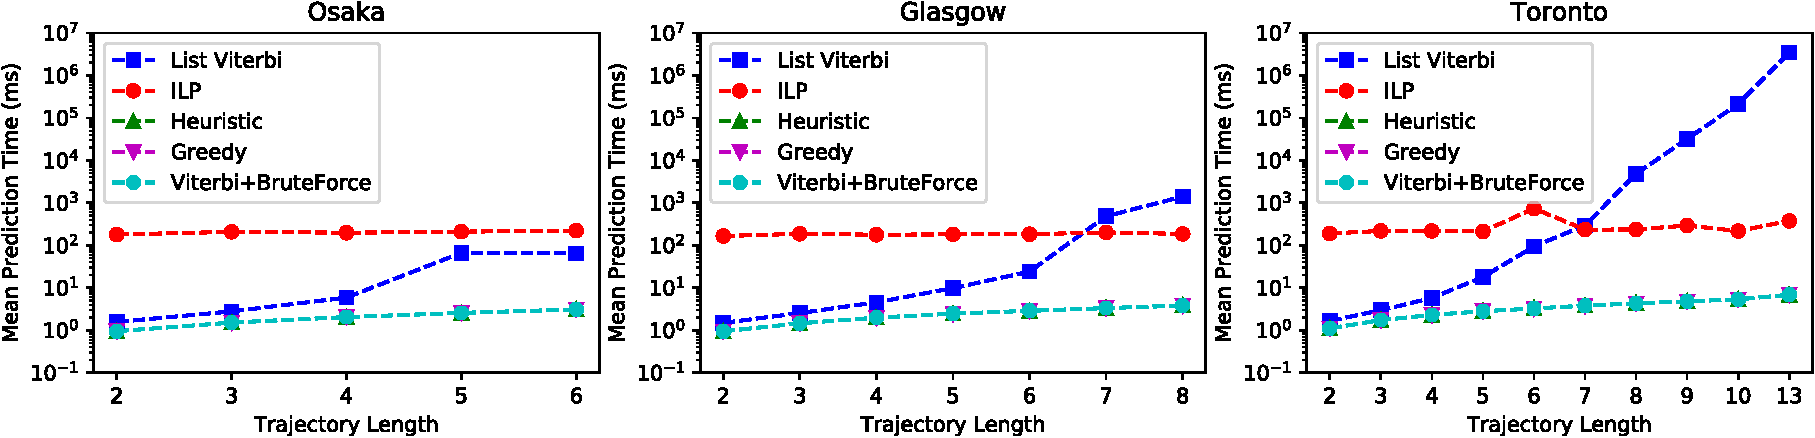
\includegraphics[width=\textwidth]{top1_inftime.pdf}
	    \captionof{figure}{Prediction time for three inference algorithms (in milliseconds)}
	    \label{fig:inftime}
	    %\captionmoveup\eqmoveup
%\end{figure*}%
%\begin{figure*}[!t]
		\quad
		\centering
		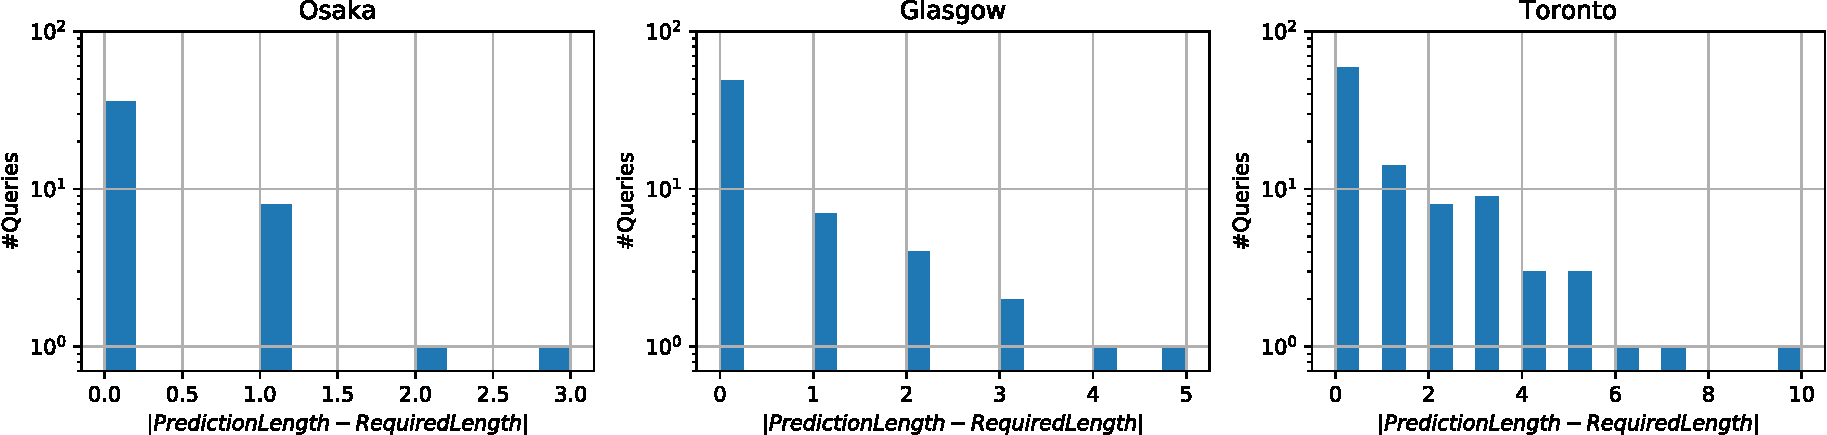
\includegraphics[width=\textwidth]{heu_lengthdiff.pdf}
	    \captionof{figure}{The difference between recommendation and required sequence length.}
	    \label{fig:length-christo}
	    %\captionmoveup\eqmoveup
%\end{figure*}%
%\begin{figure*}[!t]
		\quad
		\centering
		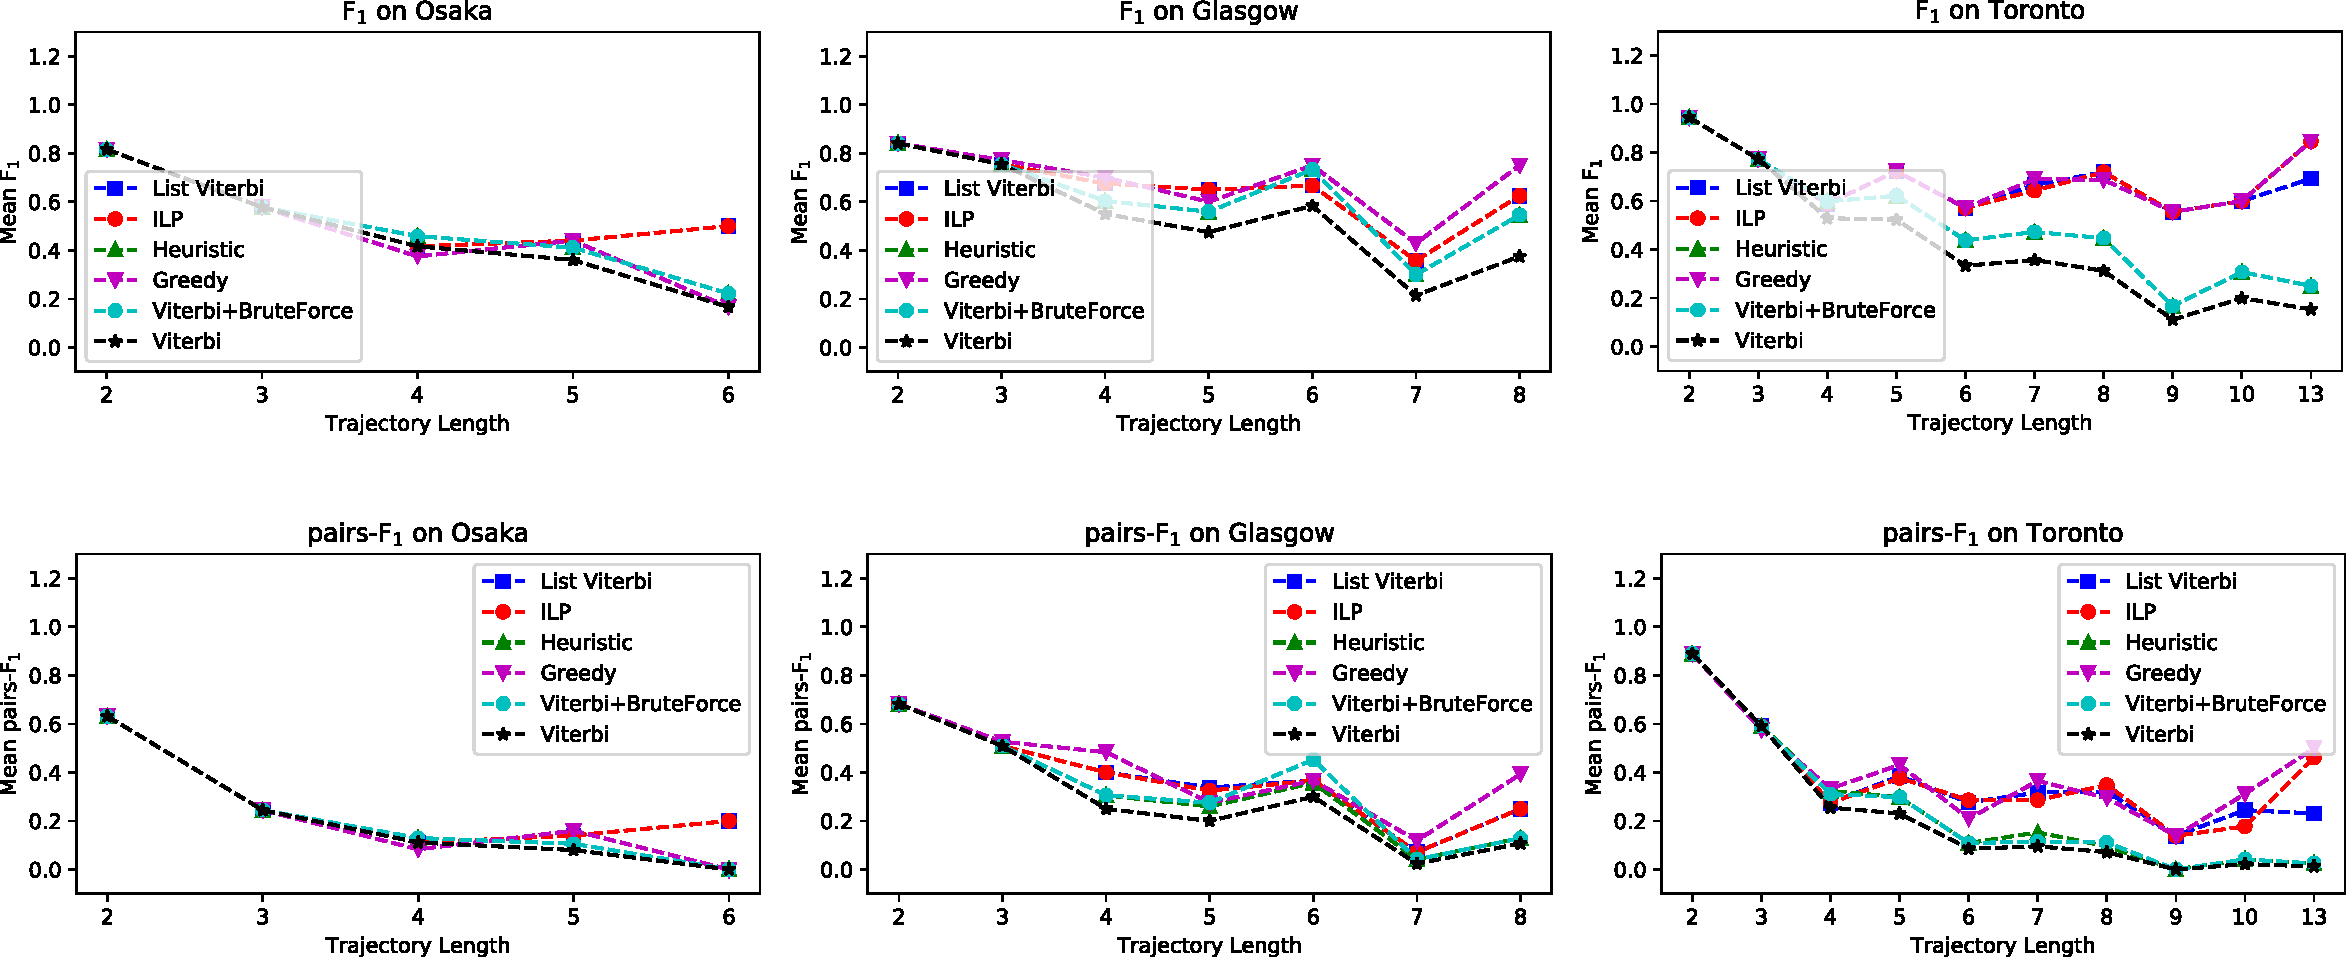
\includegraphics[width=\textwidth]{metrics.pdf}
		% 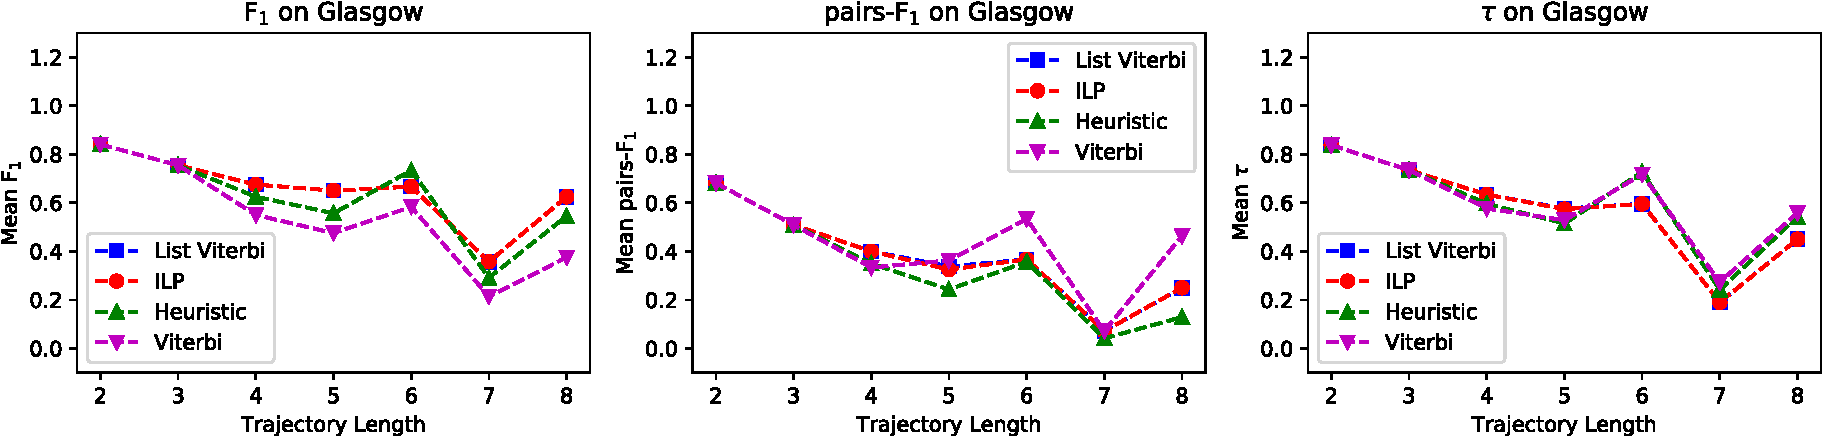
\includegraphics[width=\textwidth]{metric_d2.pdf}
		% 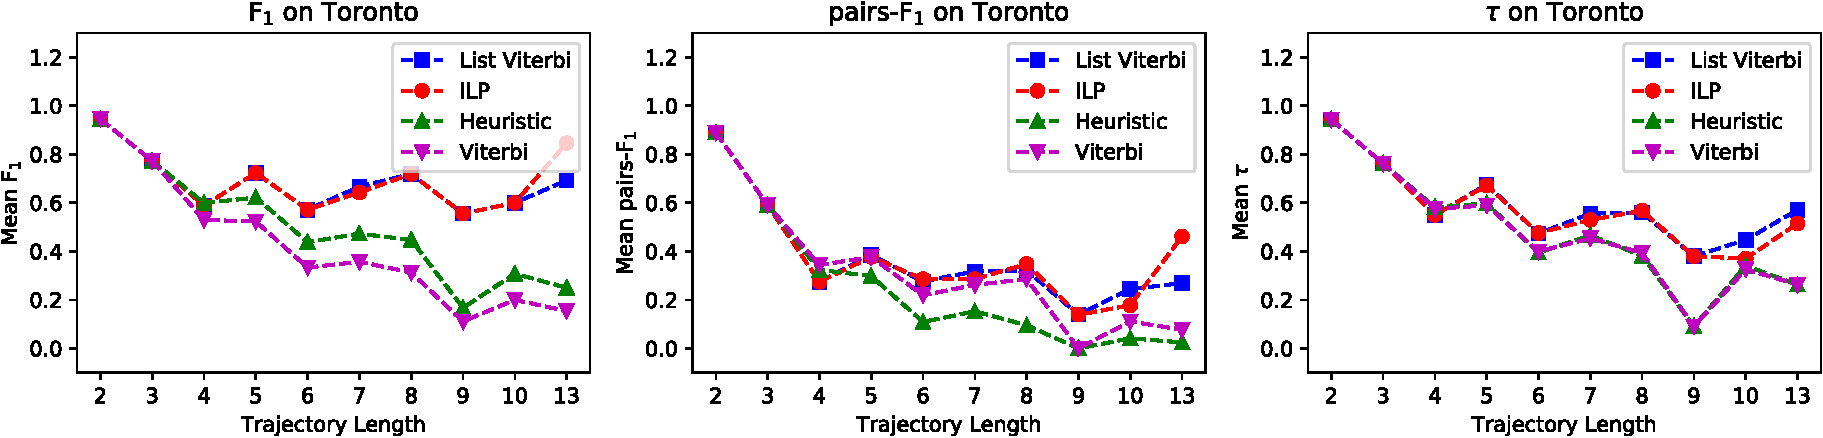
\includegraphics[width=\textwidth]{metric_d3.pdf}
	    \captionof{figure}{Accuracy versus trajectory length.}
	    \label{fig:acc-vs-length}
	    %\captionmoveup\eqmoveup
%\end{figure*}
\end{minipage}
\end{figure*}



\section{The dual problem}

\begin{equation}
\label{eq:primal}
\begin{aligned}
&\min_{\V, \W, \mubm} \ \frac{\lambda}{2} \left( \frac{1}{U} \sum_{u=1}^U \bv_u^\top \bv_u 
     + \frac{1}{N} \sum_{i=1}^N \w_i^\top \w_i + \mubm^\top \mubm \right) \\
& \hspace{4em}
     + \frac{1}{N} \sum_{i=1}^N \frac{1}{M_i^+} \sum_{m: y_i^m = 1} \ell \left( (\bv_{u(i)} + \w_i + \mubm)^\top \x^m 
     - \max_{n: y_i^n = 0} (\bv_{u(i)} + \w_i + \mubm)^\top \x^n \right).
\end{aligned}
\end{equation}

Let 
\begin{equation*}
\begin{aligned}
f_0(\V, \W, \mubm, \xibm) &= \frac{\lambda}{2} \left( \frac{1}{U} \sum_{u=1}^U \bv_u^\top \bv_u 
     + \frac{1}{N} \sum_{i=1}^N \w_i^\top \w_i + \mubm^\top \mubm \right) \\
& \quad \ 
     + \frac{1}{N} \sum_{i=1}^N \frac{1}{M_i^+} \sum_{m: y_i^m = 1} 
       \ell \left( (\bv_{u(i)} + \w_i + \mubm)^\top \x^m - \xi_i \right) \\
f_{i,n} (\V, \W, \mubm, \xibm) &= (\bv_{u(i)} + \w_i + \mubm)^\top \x^n - \xi_i, \
i \in \{1,\dots,N\}, \, n \in \{1,\dots,M\} \ \mathrm{and} \ y_i^n = 0.
\end{aligned}
\end{equation*}

Problem (\ref{eq:primal}) is equivalent to 
\begin{equation}
\label{eq:stdopt}
\begin{aligned}
\min_{\V, \W, \mubm, \xibm} \ & f_0(\V, \W, \mubm, \xibm) \\
s.t. \quad & f_{i,n}(\V, \W, \mubm, \xibm) \le 0, \
i \in \{1,\dots,N\}, \, n \in \{1,\dots,M\} \ \mathrm{and} \ y_i^n = 0.
\end{aligned}
\end{equation}

For $\beta_i^n \ge 0$, the \emph{Lagrangian} of (\ref{eq:stdopt}) is
\begin{equation*}
\begin{aligned}
L(\V, \W, \mubm, \xibm, \betabm) 
&= f_0(\V, \W, \mubm, \xibm) + \sum_{i=1}^N \sum_{n: y_i^n = 0} \beta_i^n f_{i,n} (\V, \W, \mubm, \xibm).
\end{aligned}
\end{equation*}

Note that the conjugate of the conjugate of a convex function is itself, \ie $f(\z) = f^{**}(\z) = \sup_\y \left(\z^\top \y - f^*(\y) \right)$, we have
\begin{equation*}
\begin{aligned}
\ell \left( (\bv_{u(i)} + \w_i + \mubm)^\top \x^m - \xi_i \right)
&= \sup_{\alpha_i^m} \left[ \left( (\bv_{u(i)} + \w_i + \mubm)^\top \x^m - \xi_i \right) \alpha_i^m - \ell^*(\alpha_i^m) \right],
\end{aligned}
\end{equation*}
where $\ell^*$ is the convex conjugate of surrogate loss $\ell$.

Let
\begin{equation*}
\begin{aligned}
g(\V, \W, \mubm, \xibm, \alphabm, \betabm)
&= \frac{\lambda}{2} \left( \frac{1}{U} \sum_{u=1}^U \bv_u^\top \bv_u 
     + \frac{1}{N} \sum_{i=1}^N \w_i^\top \w_i + \mubm^\top \mubm \right) \\
& \hspace{2em}
     + \sum_{i=1}^N \frac{1}{N M_i^+} \sum_{m: y_i^m = 1} \left( (\bv_{u(i)} + \w_i + \mubm)^\top \x^m - \xi_i \right) \alpha_i^m \\
& \hspace{2em}
     + \sum_{i=1}^N \sum_{n: y_i^n = 0} \beta_i^n \left( (\bv_{u(i)} + \w_i + \mubm)^\top \x^n - \xi_i \right), \\
r(\alphabm)
&= \sum_{i=1}^N \frac{1}{N M_i^+} \sum_{m: y_i^m = 1} \ell^*(\alpha_i^m),
\end{aligned}
\end{equation*}
then 
\begin{equation*}
\begin{aligned}
L(\V, \W, \mubm, \xibm, \alphabm, \betabm) 
= \sup_\alphabm \left[ g(\V, \W, \mubm, \xibm, \alphabm, \betabm) - r(\alphabm) \right].
\end{aligned}
\end{equation*}

Assuming strong duality, the \emph{Lagrangian dual function} of (\ref{eq:stdopt}) is
\begin{equation*}
\begin{aligned}
&\inf_{\V, \W, \mubm, \xibm} L(\V, \W, \mubm, \xibm, \alphabm, \betabm) \\
&= \inf_{\V, \W, \mubm, \xibm} \sup_\alphabm \left[ g(\V, \W, \mubm, \xibm, \alphabm, \betabm) - r(\alphabm) \right] \\
&= \sup_\alphabm \inf_{\V, \W, \mubm, \xibm} \left[ g(\V, \W, \mubm, \xibm, \alphabm, \betabm) - r(\alphabm) \right] \\
&= \sup_\alphabm \left[ \inf_{\V, \W, \mubm, \xibm} g(\V, \W, \mubm, \xibm, \alphabm, \betabm) - r(\alphabm) \right] \\
&= \max_\alphabm \left[ \min_{\V, \W, \mubm, \xibm} g(\V, \W, \mubm, \xibm, \alphabm, \betabm) - r(\alphabm) \right].
\end{aligned}
\end{equation*}

To solve the inner (unconstrained) minimisation, let
\begin{equation*}
\begin{aligned}
\zero &= \frac{\partial g}{\partial \bv_u} 
       = \frac{\lambda}{U} \bv_u 
         + \sum_{i \in P_u} \left( \frac{1}{N M_i^+} \sum_{m: y_i^m = 1} \alpha_i^m \x^m + \sum_{n: y_i^n = 0} \beta_i^n \x^n \right) \\
\zero &= \frac{\partial g}{\partial \w_i}
       = \frac{\lambda}{N} \w_i + \frac{1}{N M_i^+} \sum_{m: y_i^m = 1} \alpha_i^m \x^m + \sum_{n: y_i^n = 0} \beta_i^n \x^n \\
\zero &= \frac{\partial g}{\partial \mubm} 
       = \lambda \mubm + \sum_{i=1}^N \left( \frac{1}{N M_i^+} \sum_{m: y_i^m = 1} \alpha_i^m \x^m + \sum_{n: y_i^n = 0} \beta_i^n \x^n \right) \\
0     &= \frac{\partial g}{\partial \xi_i}
       = - \frac{1}{N M_i^+} \sum_{m: y_i^m = 1} \alpha_i^m - \sum_{n: y_i^n = 0} \beta_i^n \\
\end{aligned}
\end{equation*}
where $P_u$ denotes the indices of playlists from user $u$.

To simplify the notation, let $\Thetabm \in \R^{M \times N}$ such that
\begin{equation*}
\theta_i^m = 
\begin{cases}
    \frac{\alpha_i^m}{N M_i^+}, & y_i^m = 1 \\
    \beta_i^m, & y_i^m = 0, \ i \in \{1,\dots,N\}, \, m \in \{1,\dots,M\},
\end{cases}
\end{equation*}
then we have
\begin{equation*}
\begin{aligned}
\bv_u^\top &= -\frac{U}{\lambda} \sum_{i \in P_u} \thetabm_i^\top \X \\
\w_i^\top  &= -\frac{N}{\lambda} \thetabm_i^\top \X \\
\mubm^\top &= -\frac{1}{\lambda} \sum_{i=1}^N \thetabm_i^\top \X \\
\thetabm_i^\top \one_M &= 0
\end{aligned}
\end{equation*}

Thus, we have
\begin{equation*}
\begin{aligned}
&\min_{\V, \W, \mubm, \xibm} g(\V, \W, \mubm, \xibm, \alphabm, \betabm) \\
&= \frac{\lambda}{2} \left( \frac{1}{U} \sum_{u=1}^U \bv_u^\top \bv_u 
     + \frac{1}{N} \sum_{i=1}^N \w_i^\top \w_i + \mubm^\top \mubm \right) \\
& \hspace{2em}
     + \sum_{i=1}^N \left( 
       \sum_{m: y_i^m = 1} \frac{\alpha_i^m}{N M_i^+} (\bv_{u(i)} + \w_i + \mubm)^\top \x^m 
     + \sum_{n: y_i^n = 0} \beta_i^n (\bv_{u(i)} + \w_i + \mubm)^\top \x^n \right) \\
& \hspace{2em}
     - \sum_{i=1}^N \xi_i \left( \sum_{m: y_i^m = 1} \frac{\alpha_i^m}{N M_i^+} + \sum_{n: y_i^n = 0} \beta_i^n \right) \\
%   + \sum_{u=1}^U \sum_{i \in P_u} \sum_{m = 1}^M \theta_i^m \left( (\bv_u + \w_i + \mubm)^\top \x^m - \xi_i \right) \\
&= \frac{\lambda}{2} \left( \frac{1}{U} \sum_{u=1}^U \bv_u^\top \bv_u 
     + \frac{1}{N} \sum_{i=1}^N \w_i^\top \w_i + \mubm^\top \mubm \right)
     + \sum_{i=1}^N \sum_{m=1}^M \theta_i^m (\bv_{u(i)} + \w_i + \mubm)^\top \x^m
\end{aligned}
\end{equation*}

Note that
\begin{equation*}
\begin{aligned}
&\sum_{i=1}^N \sum_{m=1}^M \theta_i^m (\bv_{u(i)} + \w_i + \mubm)^\top \x^m \\
&= \sum_{i=1}^N (\bv_{u(i)} + \w_i + \mubm)^\top \left( \sum_{m=1}^M \theta_i^m \x^m \right) \\
&= \sum_{i=1}^N (\bv_{u(i)} + \w_i + \mubm)^\top \left( \thetabm_i^\top \X \right)^\top \\
&= \sum_{i=1}^N \bv_{u(i)}^\top \left( \thetabm_i^\top \X \right)^\top 
     + \sum_{i=1}^N \w_i^\top \left( \thetabm_i^\top \X \right)^\top 
     + \mubm^\top \left( \sum_{i=1}^N \thetabm_i^\top \X \right)^\top \\
&= \sum_{u=1}^U \sum_{i \in P_u} \bv_u^\top \left( \thetabm_i^\top \X \right)^\top
     - \frac{\lambda}{N} \sum_{i=1}^N \w_i^\top \w_i 
     - \lambda \mubm^\top \mubm \\
&= \sum_{u=1}^U \bv_u^\top \left( \sum_{i \in P_u} \thetabm_i^\top \X \right)^\top
     - \frac{\lambda}{N} \sum_{i=1}^N \w_i^\top \w_i 
     - \lambda \mubm^\top \mubm \\
&= -\frac{\lambda}{U} \sum_{u=1}^U \bv_u^\top \bv_u
     - \frac{\lambda}{N} \sum_{i=1}^N \w_i^\top \w_i 
     - \lambda \mubm^\top \mubm \\
&= -\lambda \left( \frac{1}{U} \sum_{u=1}^U \bv_u^\top \bv_u
     + \frac{1}{N} \sum_{i=1}^N \w_i^\top \w_i 
     + \mubm^\top \mubm \right)
\end{aligned}
\end{equation*}

As a result,
\begin{equation*}
\begin{aligned}
&\min_{\V, \W, \mubm, \xibm} g(\V, \W, \mubm, \xibm, \alphabm, \betabm) \\
&= \frac{\lambda}{2} \left( \frac{1}{U} \sum_{u=1}^U \bv_u^\top \bv_u 
     + \frac{1}{N} \sum_{i=1}^N \w_i^\top \w_i + \mubm^\top \mubm \right)
     -\lambda \left( \frac{1}{U} \sum_{u=1}^U \bv_u^\top \bv_u + \frac{1}{N} \sum_{i=1}^N \w_i^\top \w_i + \mubm^\top \mubm \right) \\
&= -\frac{\lambda}{2} \left( \frac{1}{U} \sum_{u=1}^U \bv_u^\top \bv_u + \frac{1}{N} \sum_{i=1}^N \w_i^\top \w_i + \mubm^\top \mubm \right) \\
&= -\frac{1}{2 \lambda} \left[
     U \sum_{u=1}^U \left( \sum_{i \in P_u} \thetabm_i^\top \X \right)^\top \left( \sum_{i \in P_u} \thetabm_i^\top \X \right)
   + N \sum_{i=1}^N \left( \thetabm_i^\top \X \right)^\top \left( \thetabm_i^\top \X \right)
   + \left( \sum_{i=1}^N \thetabm_i^\top \X \right)^\top \left( \sum_{i=1}^N \thetabm_i^\top \X \right) \right]
\end{aligned}
\end{equation*}

The \emph{Lagrangian dual problem} of (\ref{eq:stdopt}) is 
\begin{equation*}
\begin{aligned}
&\max_{\betabm} \inf_{\V, \W, \mubm, \xibm} L(\V, \W, \mubm, \xibm, \alphabm, \betabm) \\
&= \max_{\alphabm, \betabm} \left[ \min_{\V, \W, \mubm, \xibm} g(\V, \W, \mubm, \xibm, \alphabm, \betabm) - r(\alphabm) \right] \\
&= \min_{\Thetabm} \ \frac{1}{2 \lambda} \left[
     U \sum_{u=1}^U \left( \sum_{i \in P_u} \thetabm_i^\top \X \right)^\top \left( \sum_{i \in P_u} \thetabm_i^\top \X \right)
   + N \sum_{i=1}^N \left( \thetabm_i^\top \X \right)^\top \left( \thetabm_i^\top \X \right)
   + \left( \sum_{i=1}^N \thetabm_i^\top \X \right)^\top \left( \sum_{i=1}^N \thetabm_i^\top \X \right) \right] \\
& \hspace{4em}
   + r(\alphabm)
\end{aligned}
\end{equation*}
subject to constraints $\Thetabm^\top \one_M = \zero_N$, 
and $\theta_i^n \ge 0$ where $y_i^n = 0, \, i \in \{1,\dots,N\}, \, n \in \{1,\dots,M\}.$

Lastly, if we choose the exponential surrogate $\ell(f, y) = e^{-fy}$, then
\begin{equation*}
\ell^*(\alpha) = \sup_z \left(\alpha z - \ell(z) \right) = \max_z \left(\alpha z - e^{-z} \right),
\end{equation*}
let 
\begin{equation*}
0 = \frac{\partial (\alpha z - e^{-z})}{\partial z} = \alpha + e^{-z},
\end{equation*}
so we have
\begin{equation*}
z = -\log(-\alpha),
\end{equation*}
then
\begin{equation*}
\ell^*(\alpha) = \alpha ( 1 - \log(-\alpha) ), \ \alpha \le 0.
\end{equation*}
Thus,
\begin{equation*}
\begin{aligned}
r(\alphabm)
&= \sum_{i=1}^N \frac{1}{N M_i^+} \sum_{m: y_i^m = 1} \ell^*(\alpha_i^m) \\
&= \sum_{i=1}^N \frac{1}{N M_i^+} \sum_{m: y_i^m = 1} \alpha_i^m (1 - \log(-\alpha_i^m)) \\
&= \sum_{i=1}^N \sum_{m: y_i^m = 1} \frac{\alpha_i^m}{N M_i^+} \left(1 - \log \left( -\frac{\alpha_i^m}{N M_i^+} \cdot N M_i^+ \right) \right) \\
&= \sum_{i=1}^N \sum_{m: y_i^m = 1} \theta_i^m \left(1 - \log(-\theta_i^m) - \log(N M_i^+) \right) \\
&= \sum_{i=1}^N \sum_{m: y_i^m = 1} \theta_i^m \left(1 - \log(-\theta_i^m) - \log(N M_i^+) \right) \\
&= \sum_{i=1}^N \left( \y_i \circ \thetabm_i \right)^\top 
                \left( \y_i \circ \left(\one_M - \log(N M_i^+) \one_M - \log(-\thetabm_i) \right) \right) \\
&= \sum_{i=1}^N \left( \y_i \circ \thetabm_i \right)^\top 
                \left( \one_M - \log(N M_i^+) \one_M - \log(-\thetabm_i) \right)
\end{aligned}
\end{equation*}

The Lagrangian dual problem of (\ref{eq:stdopt}) when use the exponential surrogate is
\begin{equation}
\label{eq:dual}
\begin{aligned}
\min_{\Thetabm} \ & \frac{1}{2 \lambda} \left[
     U \sum_{u=1}^U \left( \sum_{i \in P_u} \thetabm_i^\top \X \right)^\top \left( \sum_{i \in P_u} \thetabm_i^\top \X \right)
   + N \sum_{i=1}^N \left( \thetabm_i^\top \X \right)^\top \left( \thetabm_i^\top \X \right)
   + \left( \sum_{i=1}^N \thetabm_i^\top \X \right)^\top \left( \sum_{i=1}^N \thetabm_i^\top \X \right) \right] \\
& \hspace{1em}
   + \sum_{i=1}^N \left( \y_i \circ \thetabm_i \right)^\top 
     \left( \one_M - \log(N M_i^+) \one_M - \log(-\thetabm_i) \right) \\
s.t. \ & \Thetabm^\top \one_M = \zero_N \\
           & \theta_i^n \ge 0, \, i \in \{1,\dots,N\}, \, n \in \{1,\dots,M\} \ \mathrm{and} \ y_i^n = 0.
\end{aligned}
\end{equation}



\bibliographystyle{splncs}
\bibliography{ref}

%\appendix
%\section{The dual problem of bipartite ranking with multitask regularisation}

\begin{equation}
\label{eq:mtopt}
\begin{aligned}
\min_{\W} \ \frac{C_1 + 2C_2}{2 N} \sum_{i=1}^{N} \w_i^\top \w_i 
- \frac{2C_2}{N (N - 1)} \sum_{i, j \in \{1,\dots,N\}, \, i < j} \w_i^\top \w_j
+ \frac{1}{N} \sum_{i = 1}^{N} \frac{1}{M_+^i} \sum_{m: y_i^m = 1} \ell \left( \w_i^\top \x^m - \max_{n: y_i^n = 0} \w_i^\top \x^n \right).
\end{aligned}
\end{equation}

Problem (\ref{eq:mtopt}) is hard to optimise in general due to the \emph{max} operator,
a widely used trick is to form its dual problem.
Let $C_1 = \frac{C_1 + 2C_2}{2 N}$, $C_2 = \frac{-2C_2}{N (N - 1)}$ and
\begin{equation*}
\begin{aligned}
f_0(\W, \xibm) &=  C_1 \sum_{i=1}^{N} \w_i^\top \w_i + C_2 \sum_{i, j \in \{1,\dots,N\}, \, i < j} \w_i^\top \w_j
    + \sum_{i = 1}^{N} \frac{1}{N M_+^i} \sum_{m: y_i^m = 1} \ell \left( \w_i^\top \x^m - \max_{n: y_i^n = 0} \w_i^\top \x^n \right), \\
f_{i,n}(\w_i, \xi_i) &= \w_i^\top \x^n - \xi_i, \ i \in \{1,\dots,N\}, \, n \in \{1,\dots,M\} \ \mathrm{and} \ y_n^i = 0,
\end{aligned}
\end{equation*}
where $\W \in \R^{N \times D}$ is the matrix of weights.

Then problem (\ref{eq:mtopt}) is equivalent to 
\begin{equation}
\label{eq:mtstd}
\begin{aligned}
\min_{\W, \xibm} \ & f_0(\W, \xibm) \\
s.t. \ & f_{i,n}(\w_i, \xi_i) \le 0, \ i \in \{1,\dots,N\}, \, n \in \{1,\dots,M\} \ \mathrm{and} \ y_n^i = 0.
\end{aligned}
\end{equation}
Let $\nu_i^n \ge 0$, the \emph{Lagrangian} of (\ref{eq:mtstd}) is
\begin{equation*}
\begin{aligned}
L(\W, \xibm, \nubm) 
&= f_0(\W, \xibm) + \sum_{i=1}^{N} \sum_{n: y_i^n = 0} \nu_i^n \cdot f_{i,n}(\w_i, \xi_i) \\
&= C_1 \sum_{i=1}^{N} \w_i^\top \w_i + C_2 \sum_{i, j \in \{1,\dots,N\}, \, i < j} \w_i^\top \w_j
   + \sum_{i = 1}^{N} \frac{1}{N M_+^i} \sum_{m: y_i^m = 1} \ell \left( \w_i^\top \x^m - \max_{n: y_i^n = 0} \w_i^\top \x^n \right) \\
& \quad  + \sum_{i=1}^{N} \sum_{n: y_i^n = 0} \nu_i^n \left( \w_i^\top \x^n - \xi_i \right) \\
\end{aligned}
\end{equation*}
Note that the conjugate of a convex function is itself, \ie $f(\z) = f^{**}(\z) = \sup_\y \left( \z^\top \y - f^*(\y) \right)$, we have
\begin{equation*}
\begin{aligned}
\ell \left( \w_i^\top \x^m - \max_{n: y_i^n = 0} \w_i^\top \x^n \right) 
= \sup_{\alpha_i^m} \left( (\w_i^\top \x^m - \xi_i) \alpha_i^m - \ell^*(\alpha_i^m) \right),
\end{aligned}
\end{equation*}
where $\ell^*$ is the convex conjugate of surrogate loss $\ell$, then
\begin{equation*}
\begin{aligned}
L(\W, \xibm, \nubm) 
&= C_1 \sum_{i=1}^{N} \w_i^\top \w_i + C_2 \sum_{i, j \in \{1,\dots,N\}, \, i < j} \w_i^\top \w_j
   + \sum_{i = 1}^{N} \frac{1}{N M_+^i} \sum_{m: y_i^m = 1} 
     \sup_{\alpha_i^m} \left( (\w_i^\top \x^m - \xi_i) \alpha_i^m - \ell^*(\alpha_i^m) \right) \\
& \quad  + \sum_{i=1}^{N} \sum_{n: y_i^n = 0} \nu_i^n \left( \w_i^\top \x^n - \xi_i \right) \\
&= \sup_\alphabm \left[ g(\W, \xibm, \alphabm, \nubm) - r(\alphabm) \right]
\end{aligned}
\end{equation*}
where 
\begin{equation*}
\begin{aligned}
g(\W, \xibm, \alphabm, \nubm)
&= C_1 \sum_{i=1}^{N} \w_i^\top \w_i + C_2 \sum_{i < j \in \{1,\dots,N\}} \w_i^\top \w_j
   + \frac{1}{N} \sum_{i = 1}^{N} \frac{1}{M_+^i} \sum_{m: y_i^m = 1} \left( \w_i^\top \x^m - \xi_i \right) \alpha_i^m \\
& \quad + \sum_{i=1}^{N} \sum_{n: y_i^n = 0} \nu_i^n \left( \w_i^\top \x^n - \xi_i \right), \\
r(\alphabm) &= \sum_{i = 1}^{N} \frac{1}{N M_+^i} \sum_{m: y_i^m = 1} \ell^*(\alpha_i^m).
\end{aligned}
\end{equation*}

Assuming strong duality, the \emph{Lagrangian dual function} of (\ref{eq:mtstd}) is
\begin{equation*}
\begin{aligned}
\inf_{\W, \xibm} L(\W, \xibm, \alphabm, \nubm)
&= \inf_{\W, \xibm} \sup_\alphabm \left[ g(\W, \xibm, \alphabm, \nubm) - r(\alphabm) \right] \\
&= \sup_\alphabm \inf_{\W, \xibm} \left[ g(\W, \xibm, \alphabm, \nubm) - r(\alphabm) \right] \\
&= \max_\alphabm \min_{\W, \xibm} \left[ g(\W, \xibm, \alphabm, \nubm) - r(\alphabm) \right] \\
&= \max_\alphabm \left[ \min_{\W, \xibm} \, g(\W, \xibm, \alphabm, \nubm) - r(\alphabm) \right].
\end{aligned}
\end{equation*}
To solve the (unconstrained) inner minimisation, let
\begin{equation*}
\begin{aligned}
\zero_D &= \frac{\partial g}{\partial \w_k} 
   = 2C_1 \w_k + C_2 \sum_{j \in \{1,\dots,N\}, \, j \ne k} \w_j 
     + \frac{1}{N M_k^+} \sum_{m: y_k^m = 1} \alpha_k^m \x^m
     + \sum_{n: y_k^n = 0} \nu_k^n \x^n \\
0 &= \frac{\partial g}{\partial \xi_k} 
   = -\frac{1}{N M_k^+} \sum_{m: y_k^m = 1} \alpha_k^m - \sum_{n: y_k^n = 0} \nu_k^n,
   \ k \in \{1,\dots,N\}.
\end{aligned}
\end{equation*}
To simplify the notation, let $\Thetabm \in \R^{M \times N}$ such that
\begin{equation*}
\theta_k^m = \begin{cases}
\frac{\alpha_k^m}{N M_k^+}, & y_k^m = 1 \\
\nu_k^m, & y_k^m = 0, \ m \in \{1,\dots,M\}, \, k \in \{1,\dots,N\},
\end{cases}
\end{equation*}
then we have
\begin{equation*}
\begin{aligned}
\bc_k^\top \W &= -\thetabm_k^\top \X, \\
\one_M^\top \thetabm_k &= 0, \ k \in \{1,\dots,N\}
\end{aligned}
\end{equation*}
where $\bc_k \in \R^{N}$ where the $k$-th element is $2C_1$ and all other elements are $C_2$,
$\X \in \R^{M \times N}$ is the design matrix.
The equivalent matrix form is
\begin{equation}
\label{eq:wxi}
\begin{aligned}
\C^\top \W &= -\Thetabm^\top \X \\
\Thetabm^\top \one_M &= \zero_{N}
\end{aligned}
\end{equation}
where $\C \in \R^{N \times N}$ such that
\begin{equation*}
C_{ij} = \begin{cases}
2C_1, & i = j \\
C_2,  & \mathrm{otherwise}
\end{cases}
\end{equation*}
Note that $\C = \C^\top$, thus $\W = -\C^{-1} \Thetabm^\top \X$.

Observe that
\begin{equation*}
\begin{aligned}
&\min_{\W, \xibm} \, g(\W, \xibm, \alphabm, \nubm) \\
&= C_1 \sum_{i=1}^{N} \w_i^\top \w_i + C_2 \sum_{i, j \in \{1,\dots,N\}, \, i < j} \w_i^\top \w_j
   + \sum_{i = 1}^{N} \w_i^\top \left( \frac{1}{N M_+^i} \sum_{m: y_i^m = 1} \alpha_i^m \x^m + \sum_{n: y_i^n = 0} \nu_i^n \x^n \right) \\
& \quad - \sum_{i = 1}^{N} \xi_i \left( \frac{1}{N M_+^i} \sum_{m: y_i^m = 1} \alpha_i^m + \sum_{n: y_i^n = 0} \nu_i^n \right) \\
&= C_1 \sum_{i=1}^{N} \w_i^\top \w_i + C_2 \sum_{i, j \in \{1,\dots,N\}, \, i < j} \w_i^\top \w_j 
   - \sum_{i = 1}^{N} \w_i^\top \left( 2C_1 \w_i + C_2 \sum_{j \in \{1,\dots,N\}, \, j \ne i} \w_j \right) \\
%&= - C_1 \sum_{i=1}^{N} \w_i^\top \w_i - C_2 \sum_{i < j \in \{1,\dots,N\}} \w_i^\top \w_j \\
%&= - C_1 \sum_{i=1}^{N} \w_i^\top \w_i - \frac{C_2}{2} \sum_{i=1}^{N} \w_i^\top \sum_{j \ne i \in \{1,\dots,N\}} \w_j \\
%&= -\frac{1}{2} \sum_{i=1}^{N} \w_i^\top \left( 2C_1 \w_i + C_2 \sum_{j \ne i \in \{1,\dots,N\}} \w_j \right) \\
%&= -\frac{1}{2} \sum_{i=1}^{N} \w_i^\top \left( \bc_i^\top \W \right) \\
%&= \frac{1}{2} \sum_{i=1}^{N} \w_i^\top \left( \thetabm_i^\top \X \right) \\
%&= \frac{1}{2} \Thetabm^\top \X \circ \W
&= - C_1 \sum_{i=1}^{N} \w_i^\top \w_i - \frac{C_2}{2} \sum_{i=1}^{N} \sum_{j \in \{1,\dots,N\}, \, j \ne i} \w_i^\top \w_j \\
&= - \frac{1}{2} \left( 2C_1 \sum_{i=1}^{N} \w_i^\top \w_i + C_2 \sum_{i=1}^{N} \sum_{j \in \{1,\dots,N\}, \, j \ne i} \w_i^\top \w_j \right) \\
&= - \frac{1}{2} \sum_{d=1}^{D} \sum_{d'=1}^{D} \C \circ \W^\top \W \\
&= - \frac{1}{2} \sum_{d=1}^{D} \sum_{d'=1}^{D} \C \circ \left( \C^{-1} \Thetabm^\top \X \right)^\top  \left( \C^{-1} \Thetabm^\top \X \right) \\
&= - \frac{1}{2} \sum_{d=1}^{D} \sum_{d'=1}^{D} \C \circ \left( \X^\top \Thetabm (\C^{-1})^2 \Thetabm^\top \X \right), \\
\end{aligned}
\end{equation*}
where we used the fact that the inverse of a symmetric matrix (assuming invertible) is also a symmetric matrix.

Lastly, the \emph{Lagrangian dual problem} of (\ref{eq:mtstd}) is
\begin{equation}
\label{eq:mtdual}
\begin{aligned}
\max_{\alphabm, \nubm} \inf_{\W, \xibm} L(\W, \xibm, \alphabm, \nubm) 
&= \max_{\alphabm, \nubm} \left[ \min_{\W, \xibm} g(\W, \xibm, \alphabm, \nubm) - r(\alphabm) \right] \\
&= \min_{\alphabm, \nubm} \left[ \frac{1}{2} \sum_{d=1}^{D} \sum_{d'=1}^{D} \C \circ \left( \X^\top \Thetabm (\C^{-1})^2 \Thetabm^\top \X \right) 
   + r(\alphabm) \right], \\
\end{aligned}
\end{equation}
subject to constraints
\begin{equation*}
\Thetabm^\top \one_M = \zero_{N}.
\end{equation*}

If we use the exponential surrogate, \ie $\ell(fy) = e^{-fy}$, then
\begin{equation*}
\begin{aligned}
\ell^*(\alpha) = \sup_z (\alpha z - \ell(z) ) = \max_z (\alpha z - e^{-z}).
\end{aligned}
\end{equation*}
Let 
\begin{equation*}
0 = \frac{\partial (\alpha z - e^{-z})} {\partial z} = \alpha + e^{-z},
\end{equation*}
we have 
\begin{equation*}
z = -\log(-\alpha).
\end{equation*}
Thus, 
\begin{equation*}
\begin{aligned}
r(\alphabm) 
&= \sum_{i = 1}^{N} \frac{1}{N M_+^i} \sum_{m: y_i^m = 1} \ell^*(\alpha_i^m) \\
&= \sum_{i = 1}^{N} \frac{1}{N M_+^i} \sum_{m: y_i^m = 1} \left( -\alpha_i^m \log(-\alpha_i^m) + \alpha_i^m \right) \\
&= \sum_{i = 1}^{N} \sum_{m: y_i^m = 1} \frac{\alpha_i^m}{N M_+^i} \left(1 - \log \left( -\frac{\alpha_i^m}{N M_+^i} 
   \cdot N M_+^i \right) \right) \\
&= \sum_{i = 1}^{N} \sum_{m: y_i^m = 1} \theta_i^m \left( 1 - \log(-\theta_i^m) - \log(N M_+^i) \right)
\end{aligned}
\end{equation*}

\end{document}
